\documentclass[a4paper, 11pt, twoside, openright]{report}
\usepackage[top=2.5cm, bottom=2.5cm, left=2cm, right=2cm]{geometry}
\usepackage{graphicx}
\usepackage{booktabs}
\usepackage{url}
\usepackage[spanish]{babel}
\usepackage[utf8]{inputenc}
\usepackage{pdfpages}
\usepackage{hyperref}
\hypersetup{
    colorlinks,
    citecolor=black,
    filecolor=black,
    linkcolor=black,
    urlcolor=black
}
\usepackage{mathenv}
\usepackage{amsmath}
\usepackage{color}
\usepackage{caption}
\usepackage[bottom]{footmisc}
\usepackage{cancel}
\usepackage{multirow}
\usepackage[toc,page]{appendix}
\usepackage{titlesec}
\usepackage{bm}
\usepackage{mathtools}
\usepackage{subfigure}
\usepackage{cases}

\setcounter{secnumdepth}{4}
\setcounter{tocdepth}{4}



\setlength{\parskip}{1em}
\setlength{\parindent}{0em}
\titleformat{\chapter}[display]
   {\normalfont\huge\bfseries}{\chaptertitlename\ \thechapter}{0pt}{\Huge}
\renewcommand*{\arraystretch}{1.5}

\begin{document}

%Titlepage

\pagenumbering{roman}
\begin{titlepage}

	\vspace*{5.5cm}
	\centering

	%English title
	{\huge\bfseries Documentación adicional para la solicitud de la \\ \vspace*{1cm}
	                acreditación nacional para el acceso a los\\ \vspace*{1cm}
                        cuerpos docentes universitarios}
	
	\begin{flushleft}
	
	\vspace{6.6cm}
	{\Large Solicitante: \textbf{Pablo Martínez Ruiz del Árbol}\\}
	{\Large DNI: \textbf{72058705G}\\}
	{\Large Código de solicitud: \textbf{1599727061899}\\}
	{\Large Solicitud: \textbf{Titular de Universidad - Ciencias - Física}\\}
	{\Large \textbf{Agencia Nacional de Evaluación de la Calidad y Acreditación}}
	\vfill
	
	\end{flushleft}

\end{titlepage}

%Empty page
\tableofcontents
\clearpage
\thispagestyle{empty}
\phantom{a}
\vfill
\newpage

%Abstract and keywords

\setcounter{page}{1}
%Here it starts!
\pagenumbering{arabic}

\renewcommand\thechapter{\arabic{chapter}}
\renewcommand\thesection{\thechapter.\Alph{section}}
\renewcommand\thesubsection{\thesection.\arabic{subsection}}
\renewcommand\thesubsubsection{\thesubsection.\arabic{subsubsection}}

\chapter{Experiencia investigadora}

\section{Calidad y difusión de resultados de la actividad investigadora}

\subsection{Publicaciones científicas indexadas en JCR}

\subsubsection{CMS TECHNICAL DESIGN REPORT VOLUME II PHYSICS PERFORMANCE}
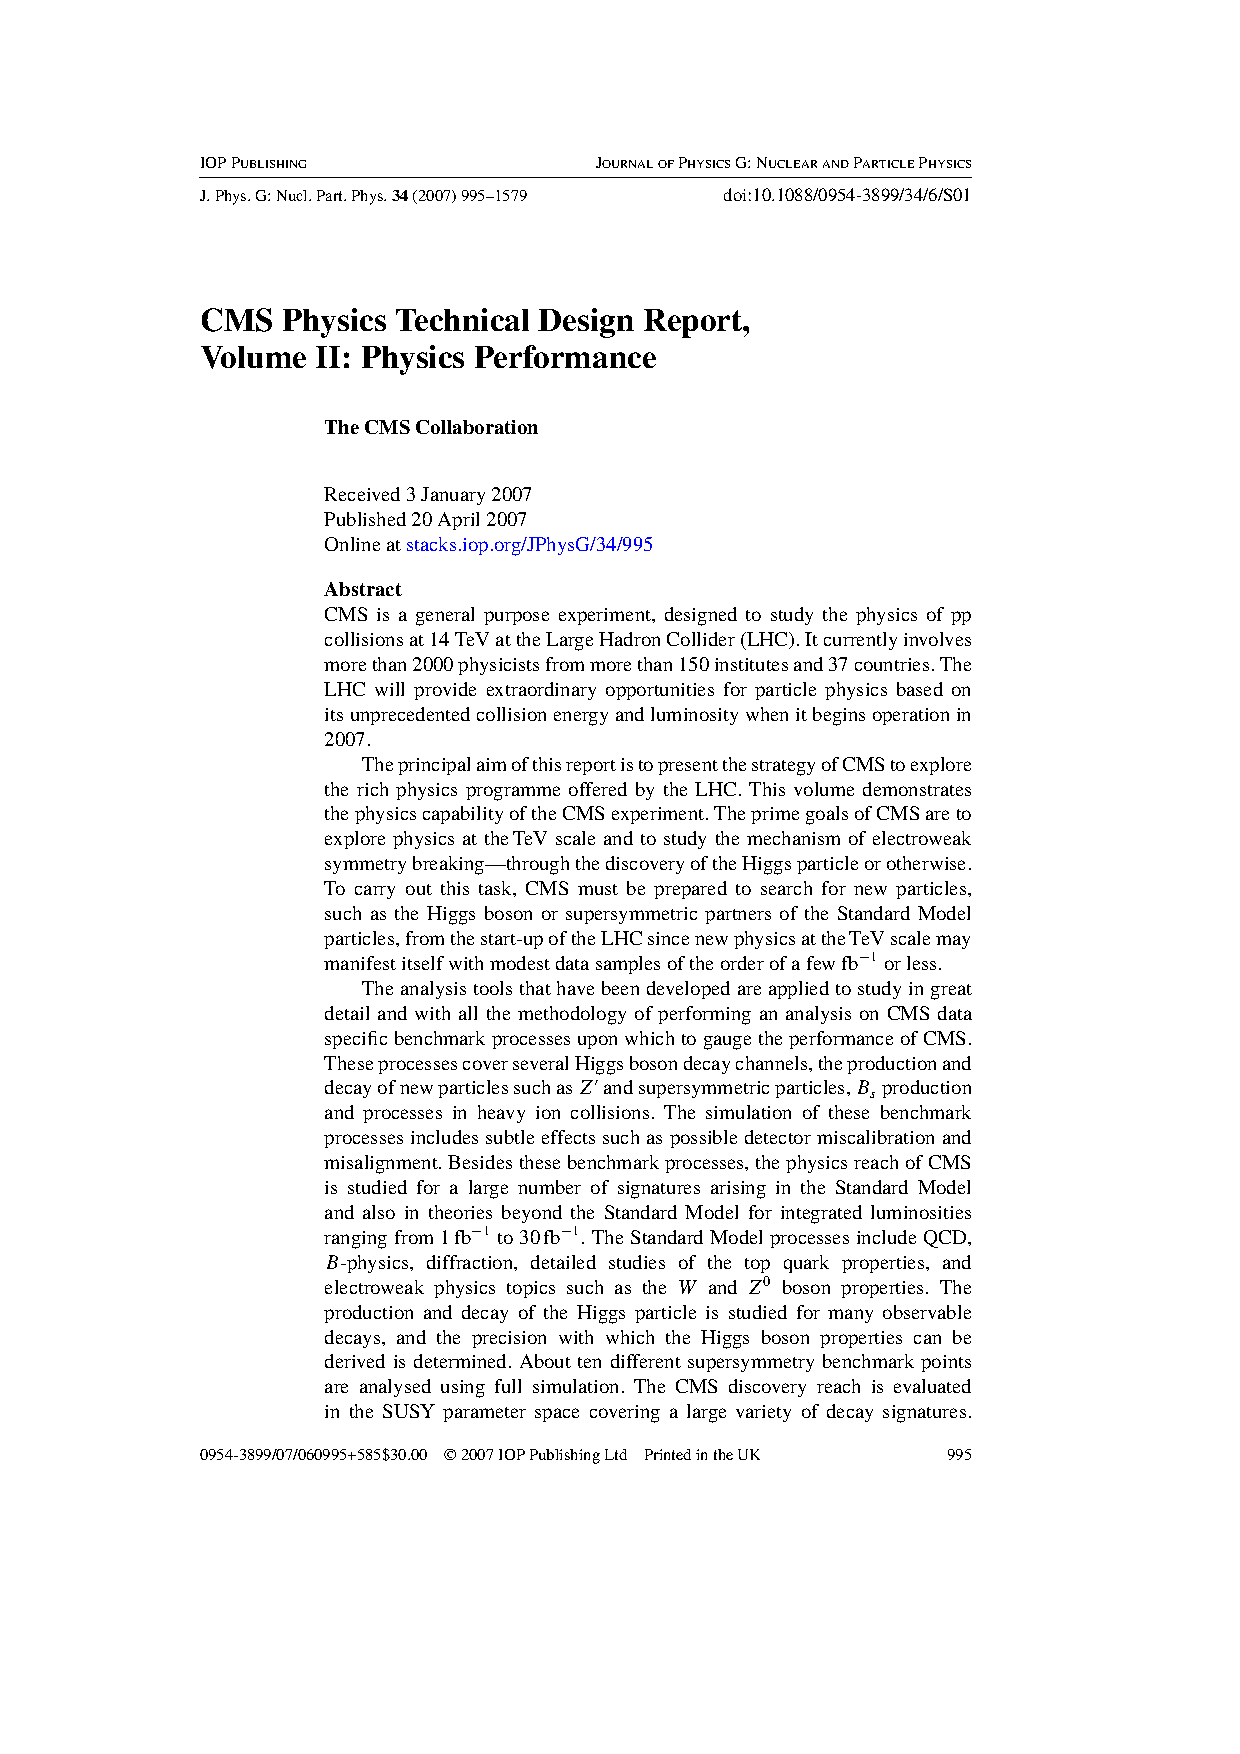
\includepdf[pages={1,2,3}]{Articulos/ArticulosReducidos/Investigacion_Publicaciones_CMS_TECHNICAL_DESIGN_REPORT_VOLUME_II_PHYSICS_PERFORMANCE.pdf}
\subsubsection{The CMS Experiment at the CERN LHC}
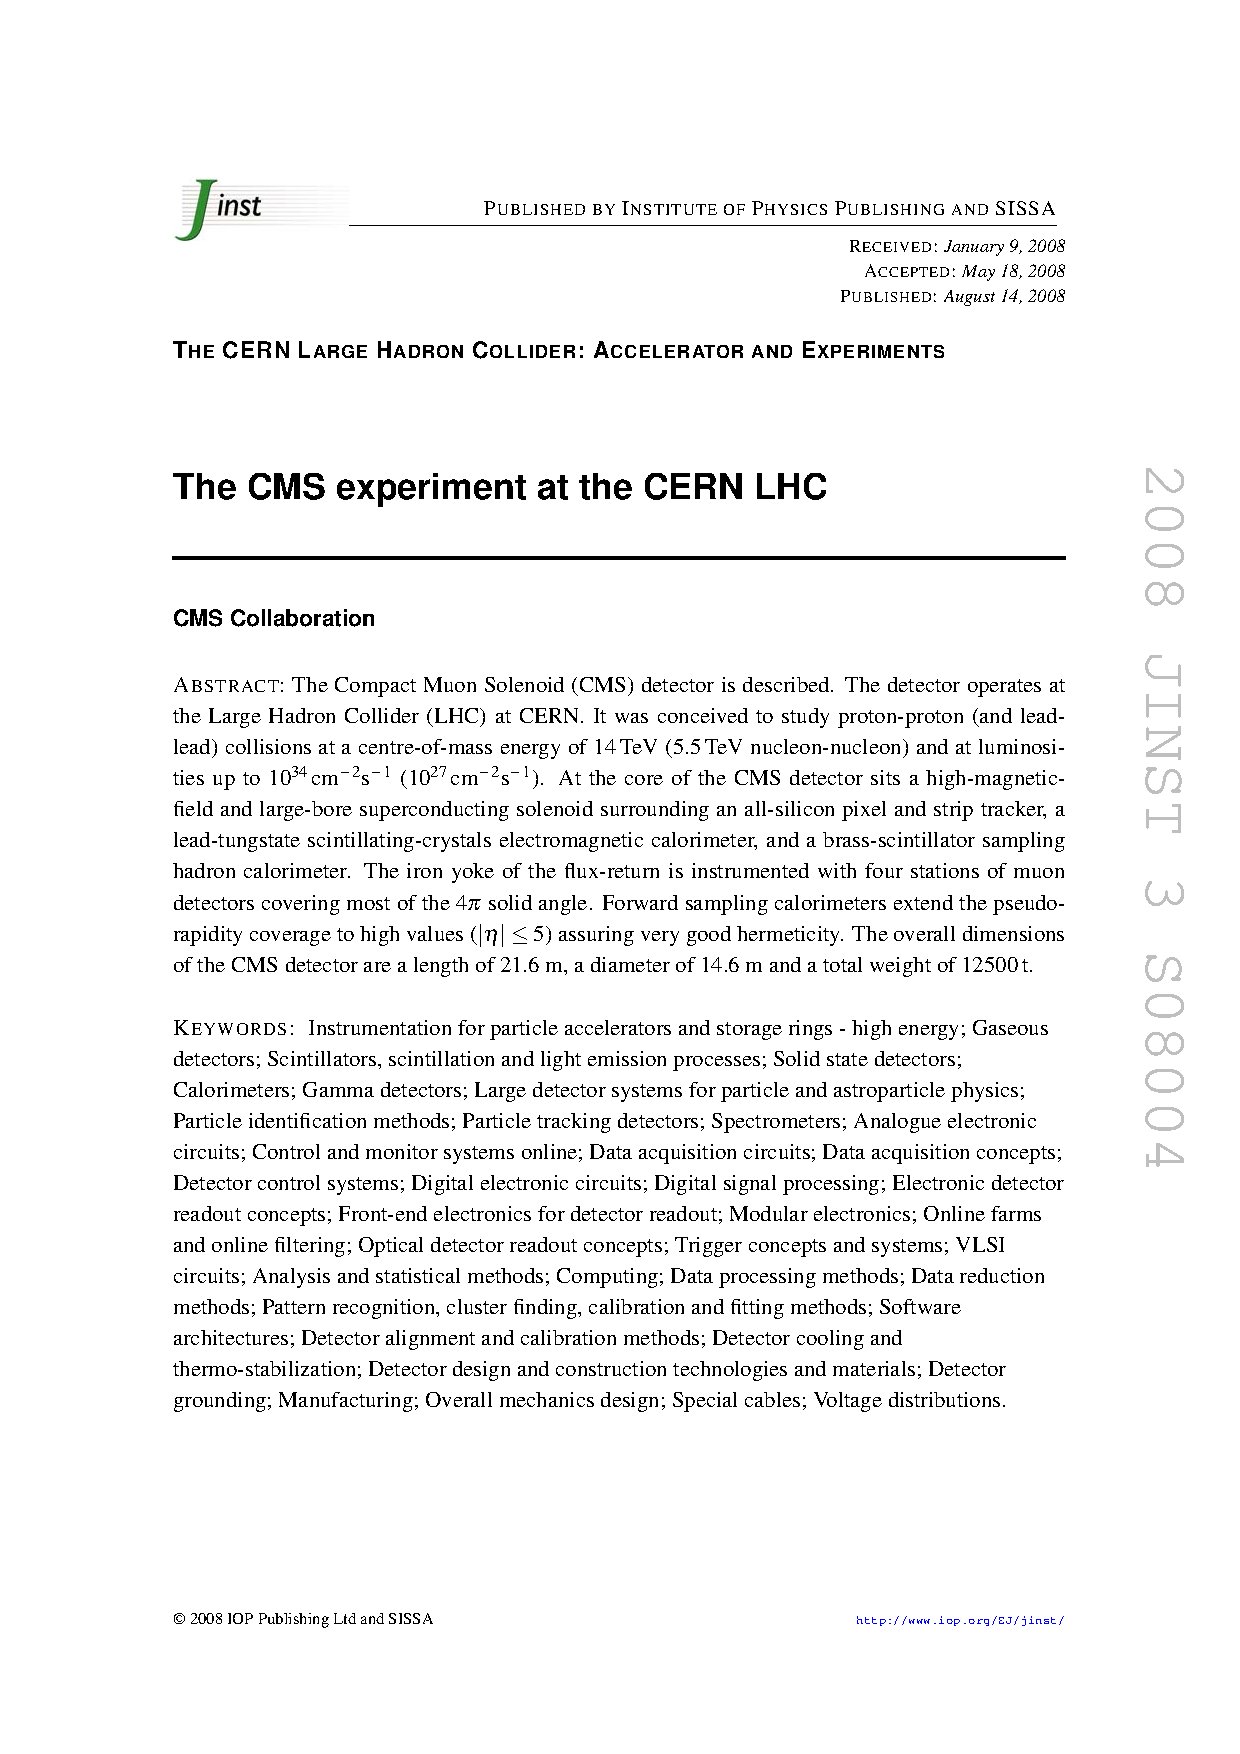
\includepdf[pages={1,2,3}]{Articulos/ArticulosReducidos/Investigacion_Publicaciones_The_CMS_Experiment_At_The_CERN_LHC.pdf}
\subsubsection{OFFLINE CALIBRATION PROCEDURE OF THE CMS DRIFT TUBE DETECTORS}
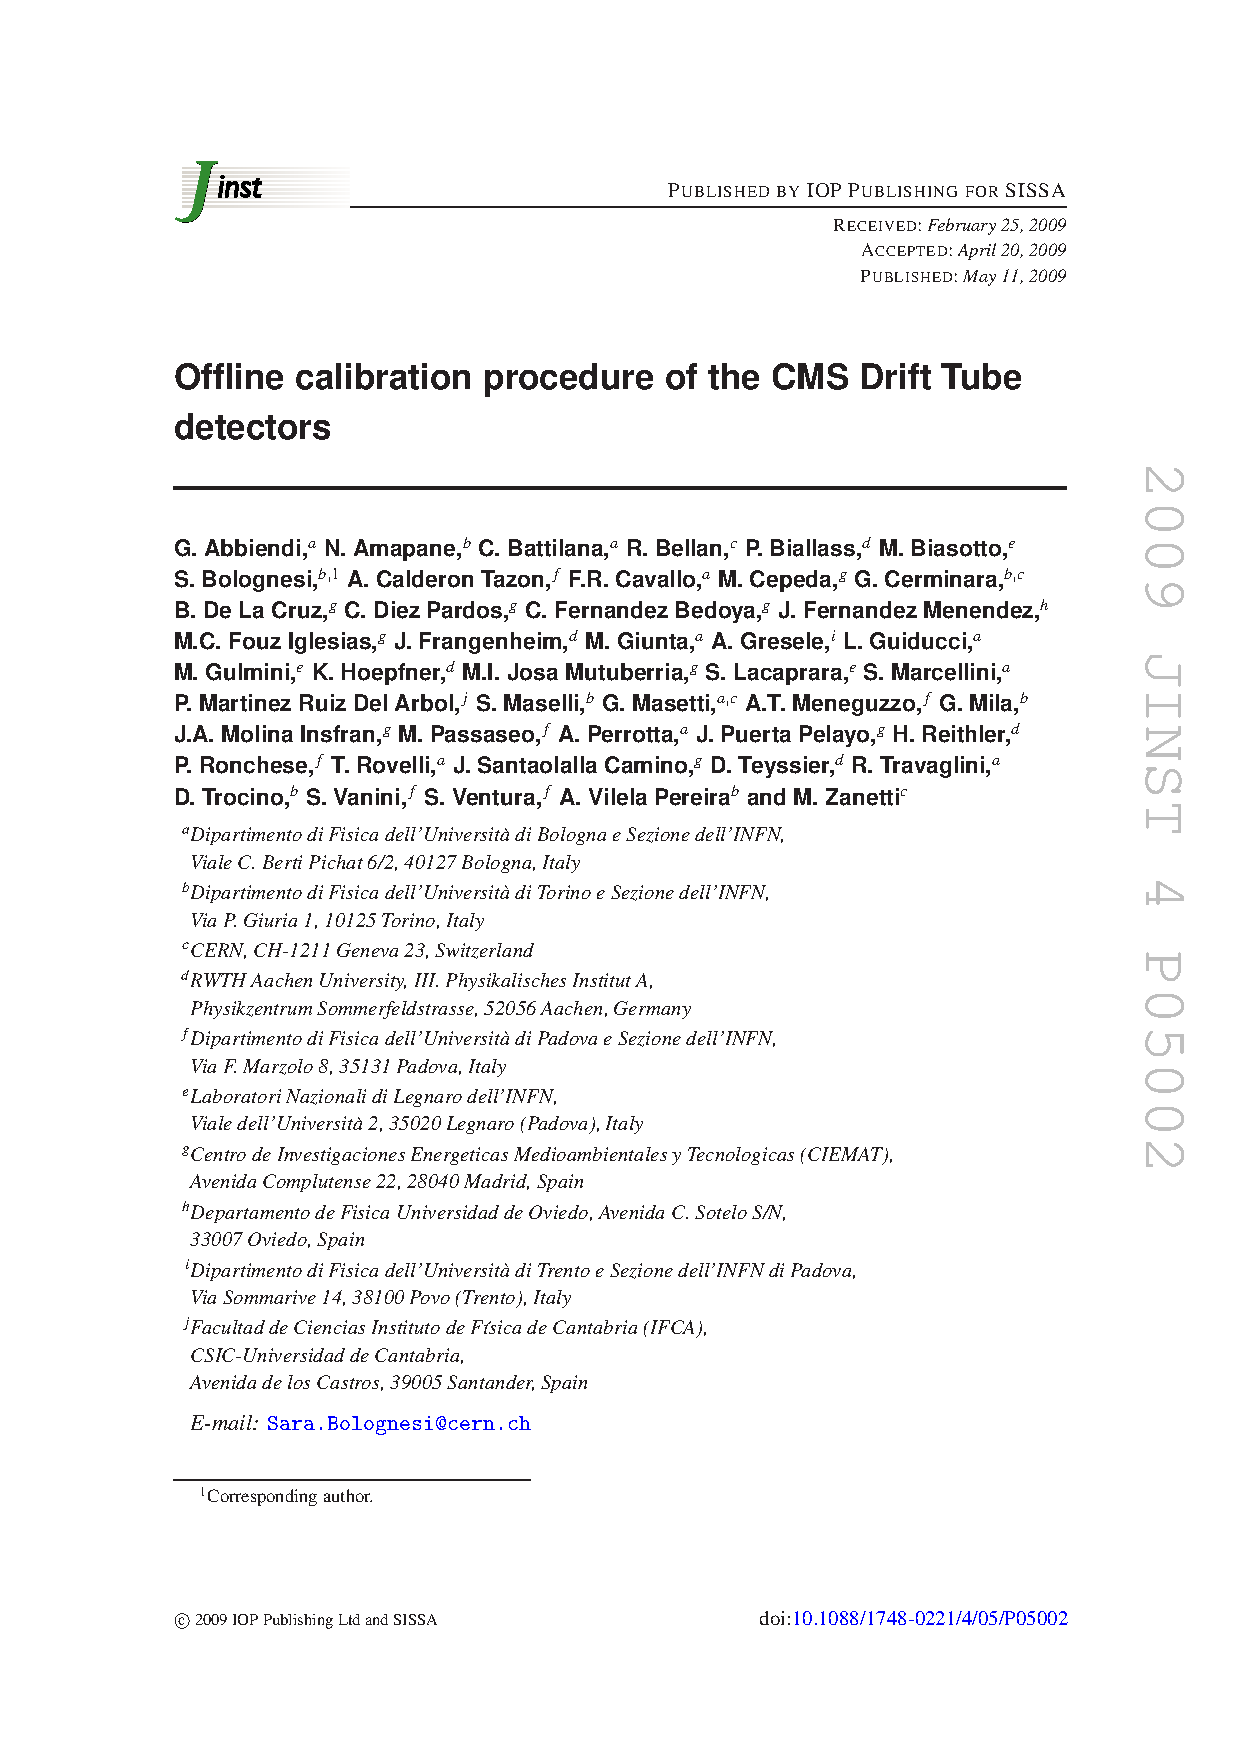
\includepdf[pages={1,2}]{Articulos/ArticulosReducidos/Investigacion_Publicaciones_OFFLINE_CALIBRATION_PROCEDURE_OF_THE_CMS_DRIFT_TUBE_DETECTORS.pdf}
\subsubsection{MOTIONS OF CMS DETECTOR STRUCTURES DUE TO THE MAGNETIC FIELD FORCES AS OBSERVED BY THE LINK ALIGNMENT SYSTEM DURING THE TEST OF THE 4 TESLA MAGNET SOLENOID}
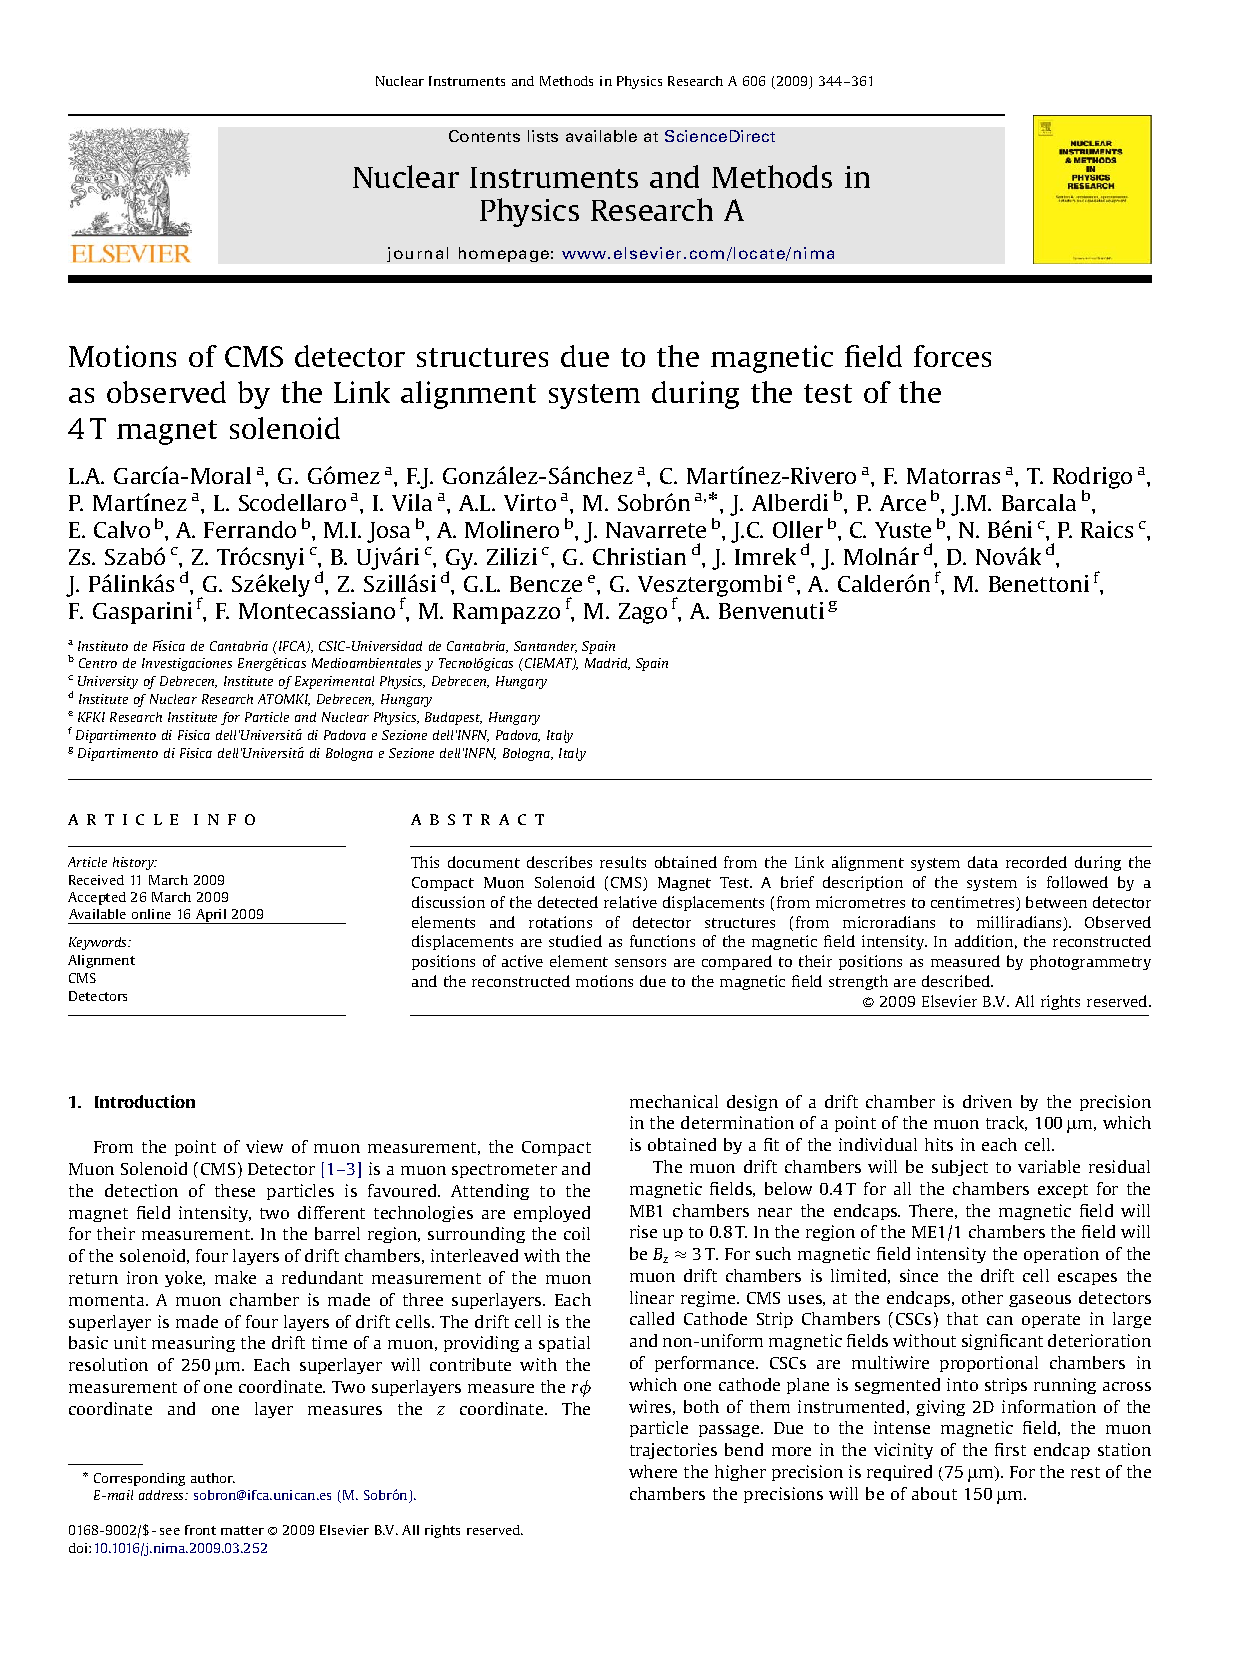
\includepdf[pages={1,2}]{Articulos/ArticulosReducidos/Investigacion_Publicaciones_MOTIONS_OF_CMS_DETECTOR_STRUCTURES_DUE_TO_THE_MAGNETIC_FIELD_FORC.pdf}
\subsubsection{CMS MUON ALIGNMENT SYSTEM DESCRIPTION AND FIRST RESULTS}
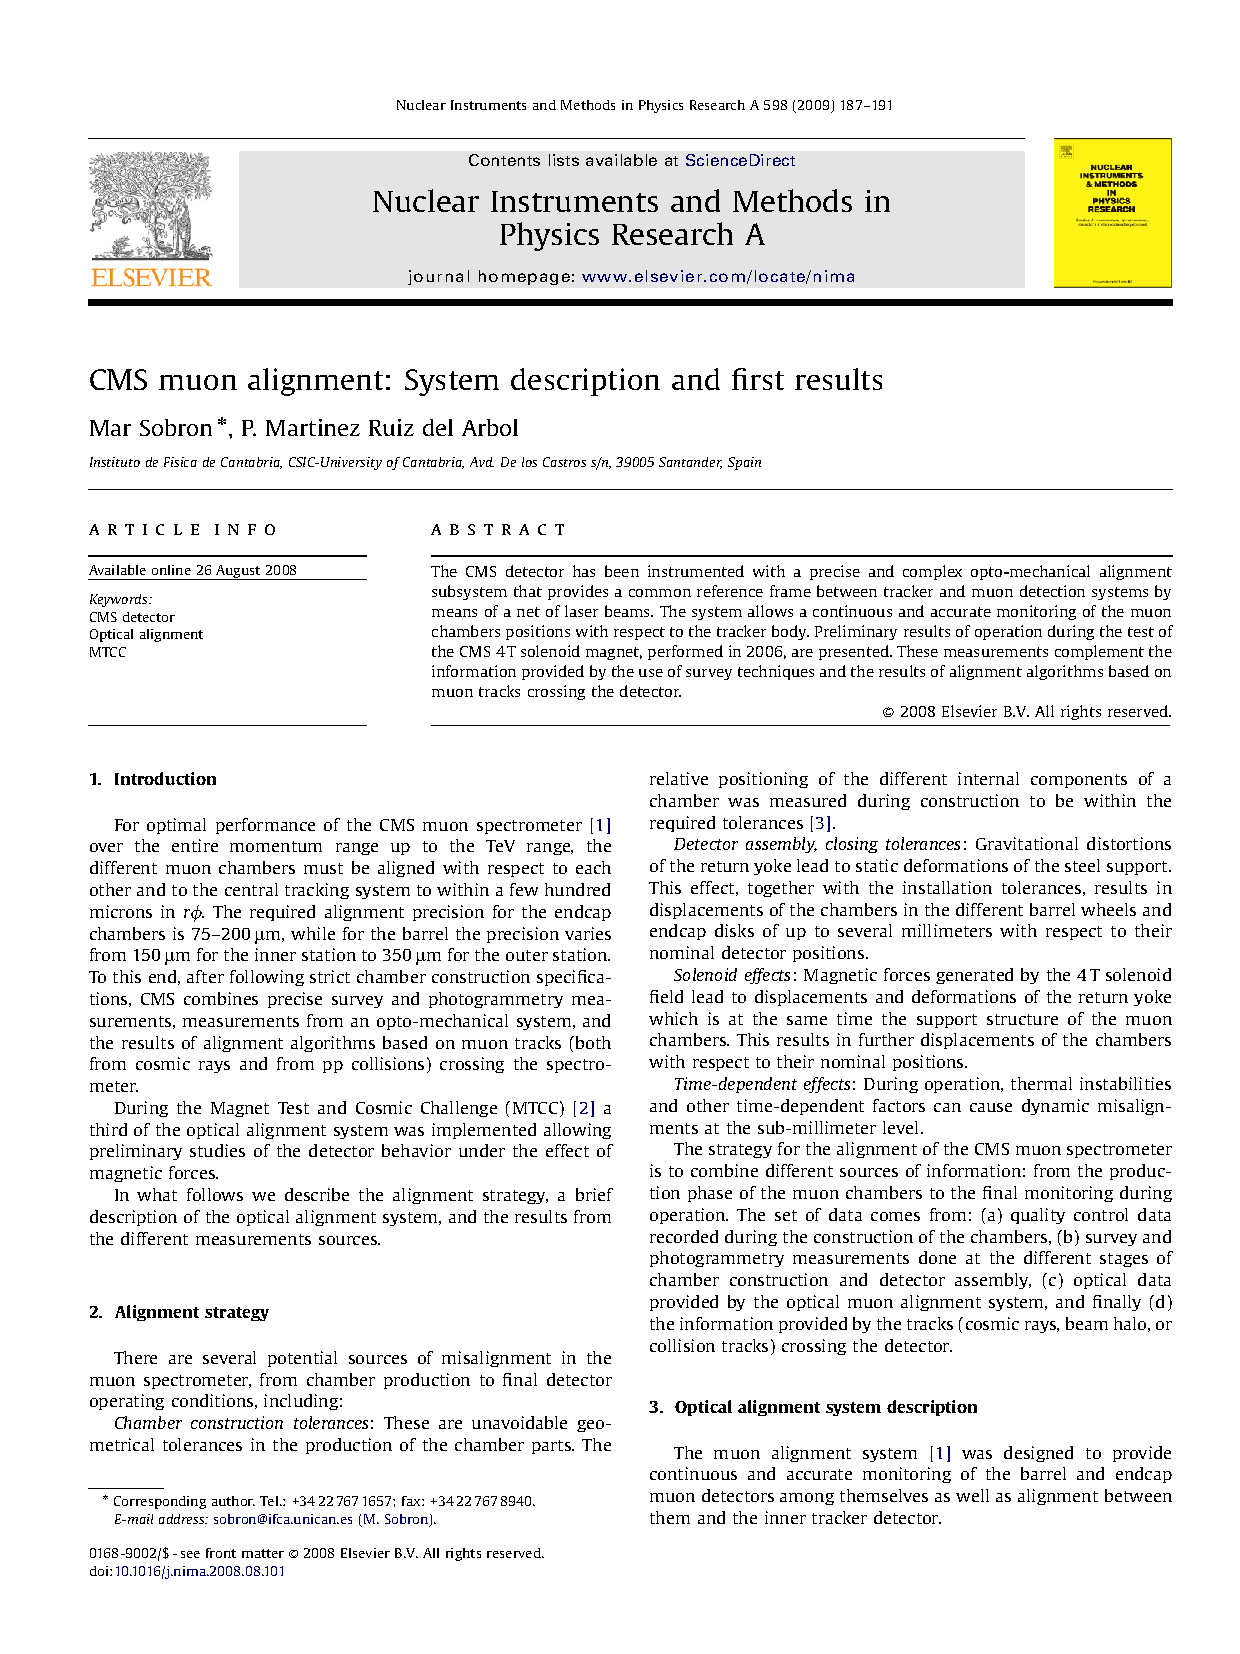
\includepdf[pages={1,2}]{Articulos/ArticulosReducidos/Investigacion_Publicaciones_CMS_MUON_ALIGNMENT_SYSTEM_DESCRIPTION_AND_FIRST_RESULTS.pdf}
\subsubsection{ALIGNING THE CMS MUON CHAMBERS WITH THE MUON ALIGNMENT SYSTEM DURING AN EXTENDED COSMIC RAY RUN}
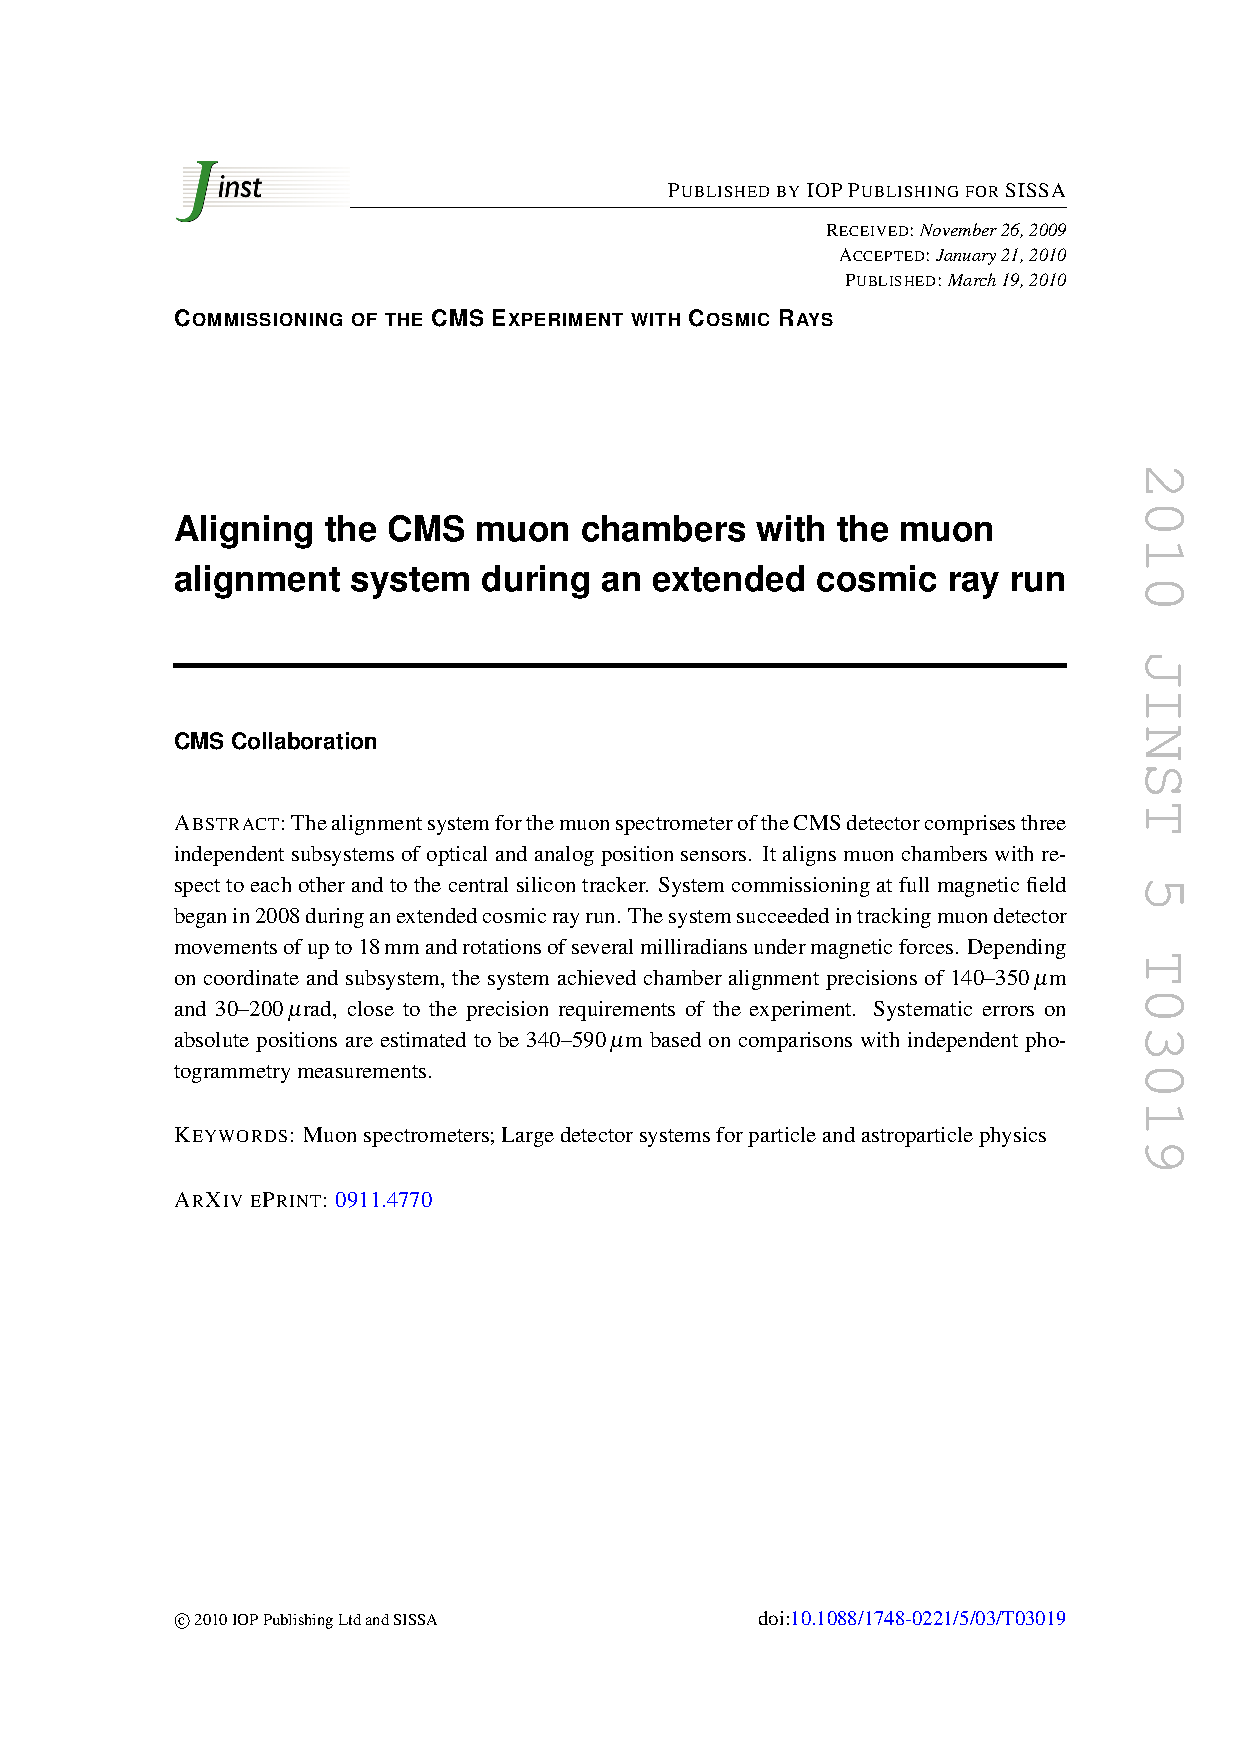
\includepdf[pages={1,2,3}]{Articulos/ArticulosReducidos/Investigacion_Publicaciones_ALIGNING_THE_CMS_MUON_CHAMBERS_WITH_THE_MUON_ALIGNMENT_SYSTEM_DUR.pdf}
\subsubsection{ALIGNMENT OF THE CMS MUON SYSTEM WITH COSMIC-RAY AND BEAM-HALO MUONS}
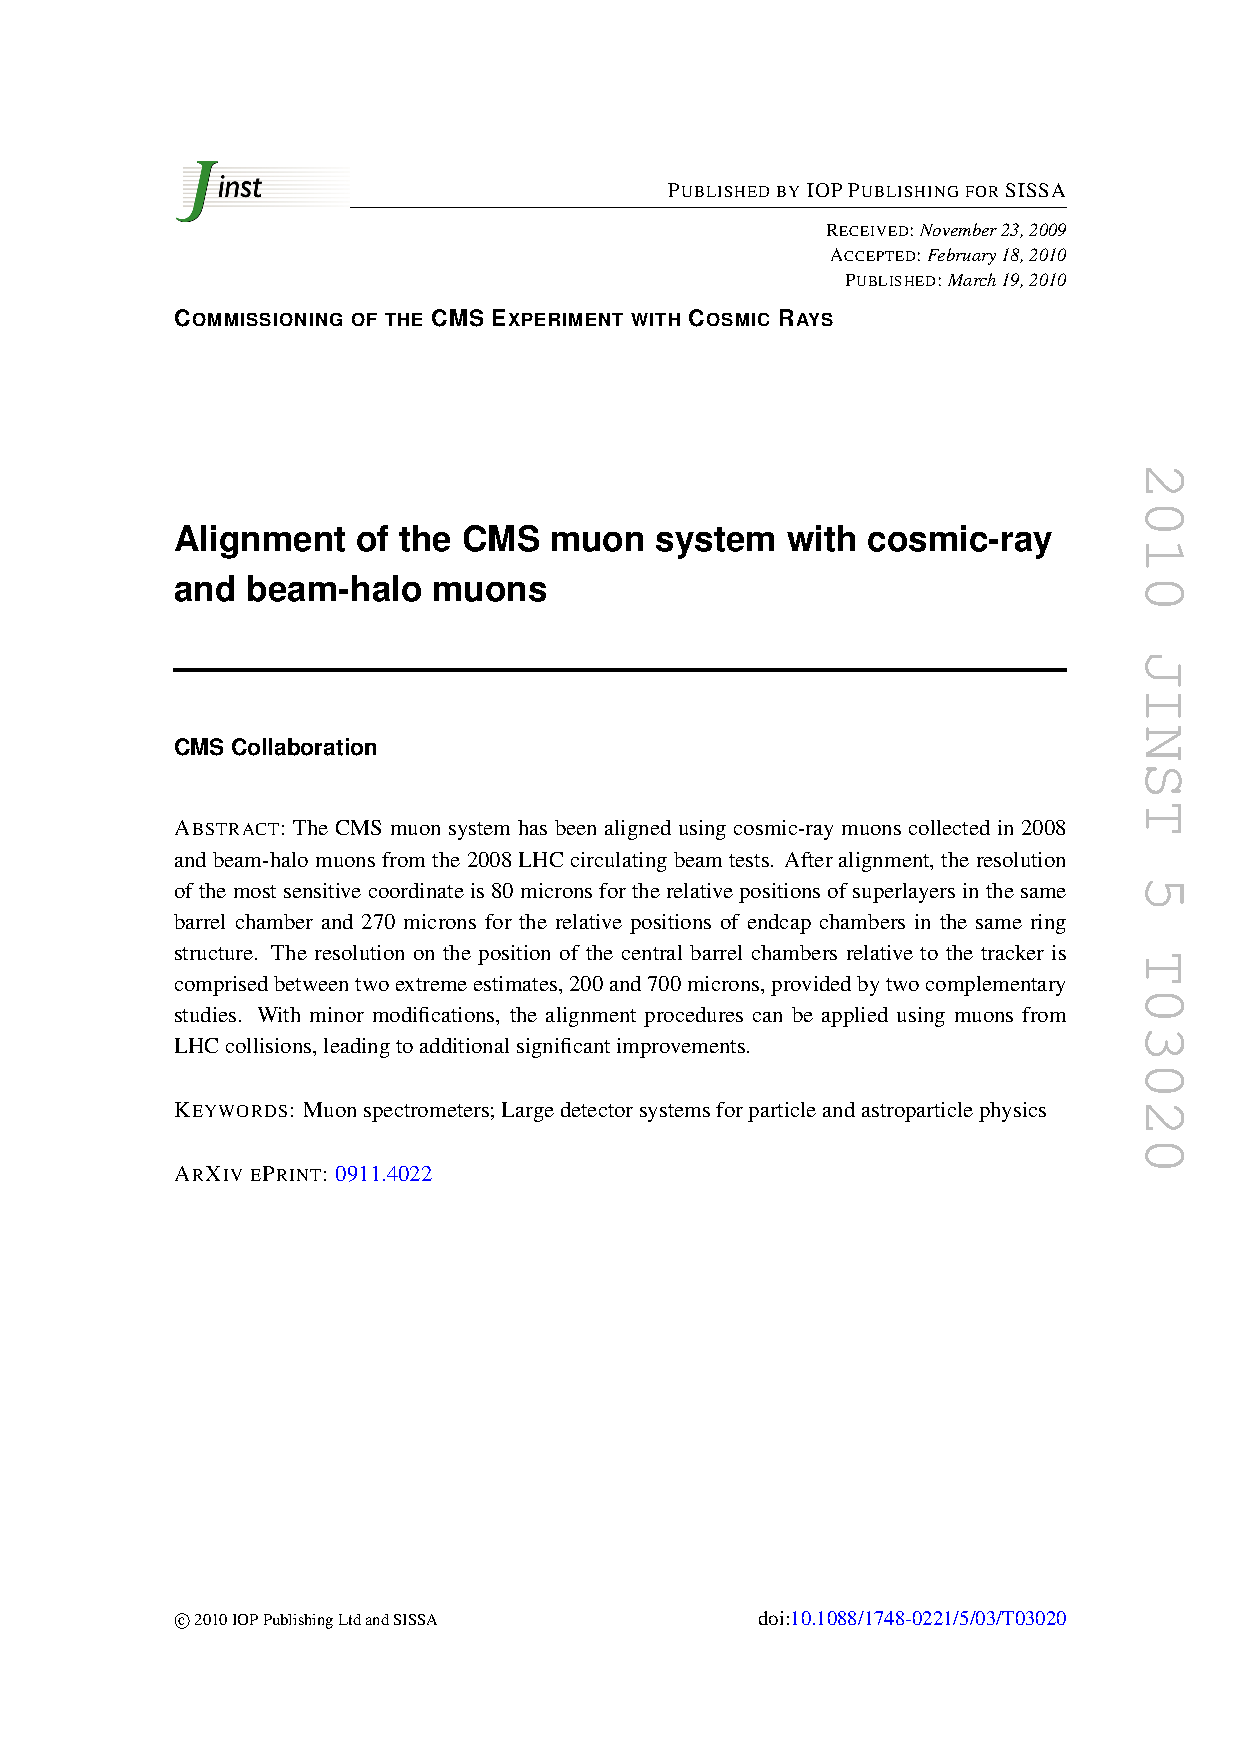
\includepdf[pages={1,2,3}]{Articulos/ArticulosReducidos/Investigacion_Publicaciones_ALIGNMENT_OF_THE_CMS_MUON_SYSTEM_WITH_COSMIC-RAY_AND_BEAM-HALO_MU.pdf}
\subsubsection{CMS DATA PROCESSING WORKFLOWS DURING AN EXTENDED COSMIC RAY RUN}
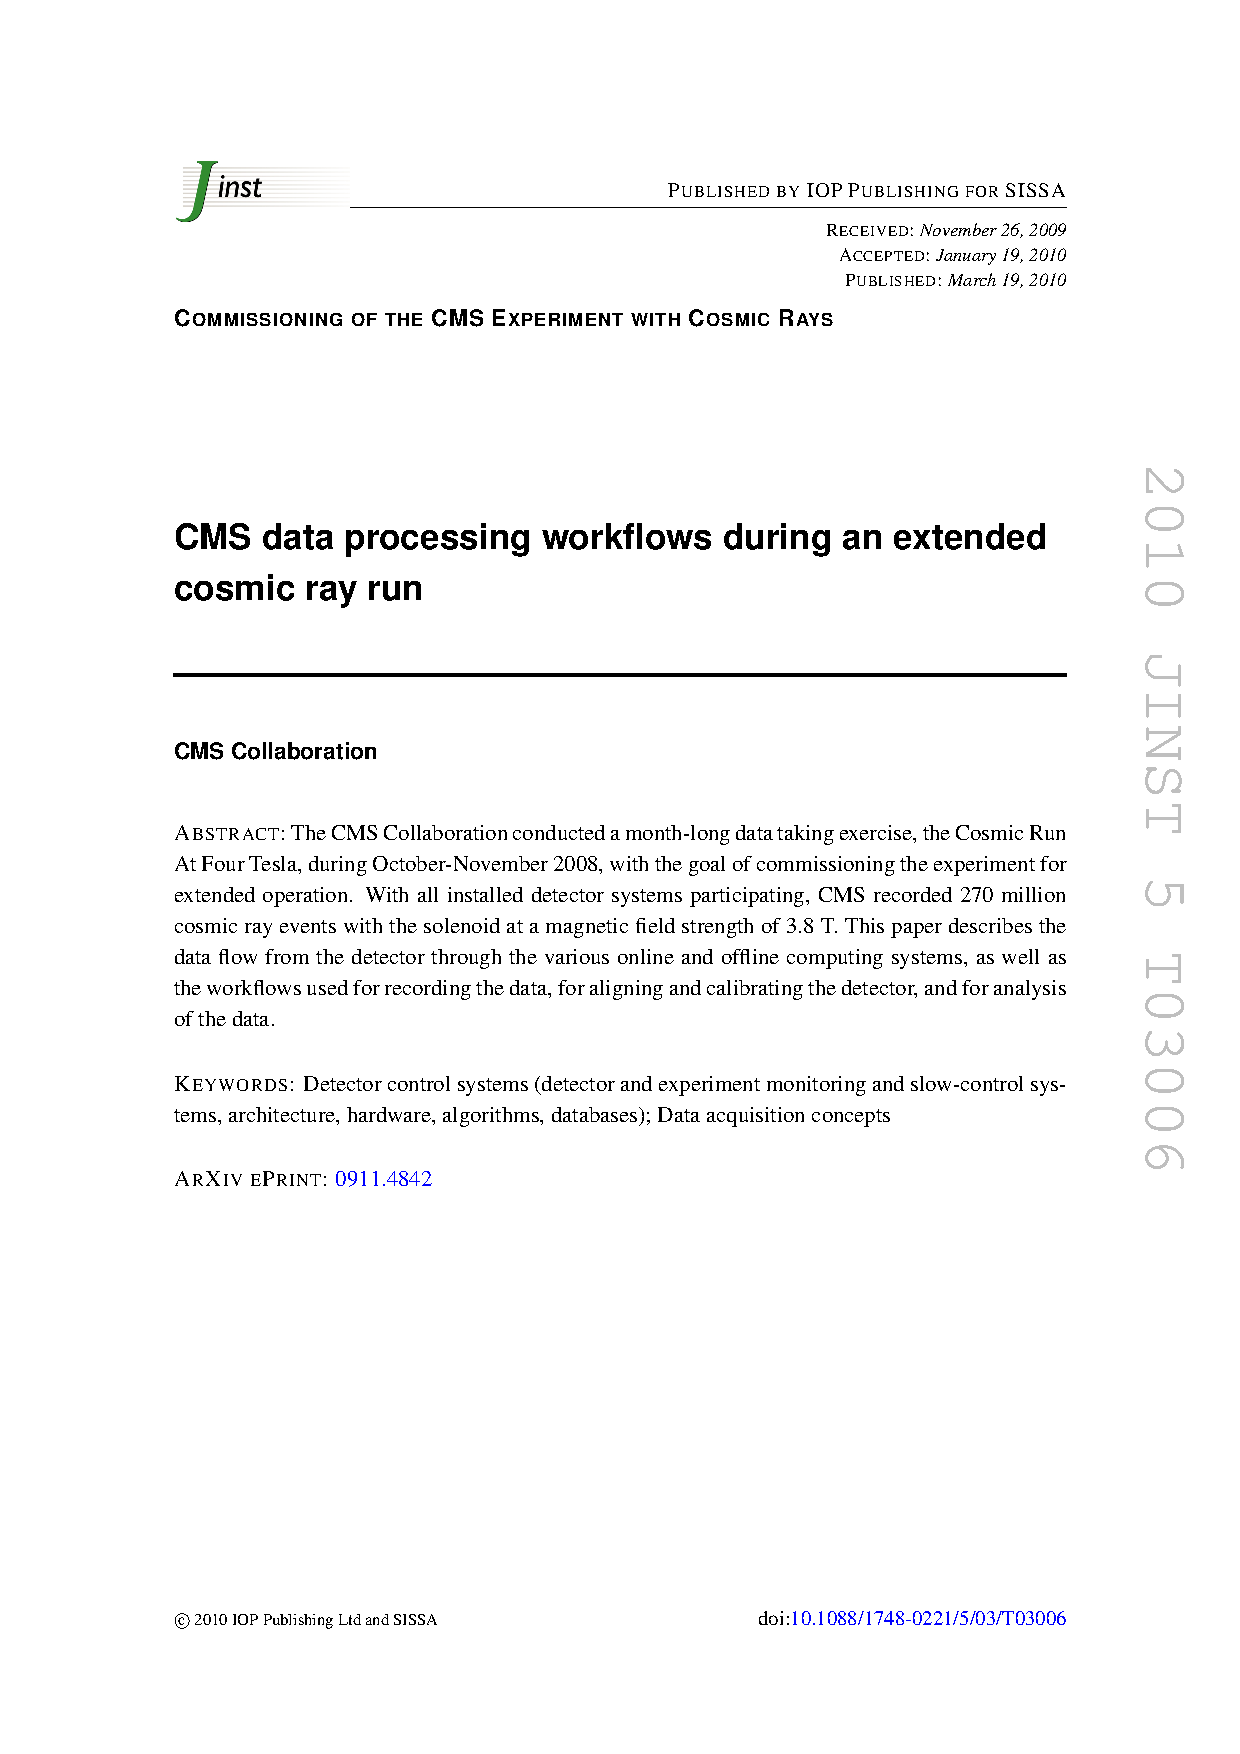
\includepdf[pages={1,2,3}]{Articulos/ArticulosReducidos/Investigacion_Publicaciones_CMS_DATA_PROCESSING_WORKFLOWS_DURING_AN_EXTENDED_COSMIC_RAY_RUN.pdf}
\subsubsection{CALIBRATION OF THE CMS DRIFT TUBE CHAMBERS AND MEASUREMENT OF THE DRIFT VELOCITY WITH COSMIC RAYS}
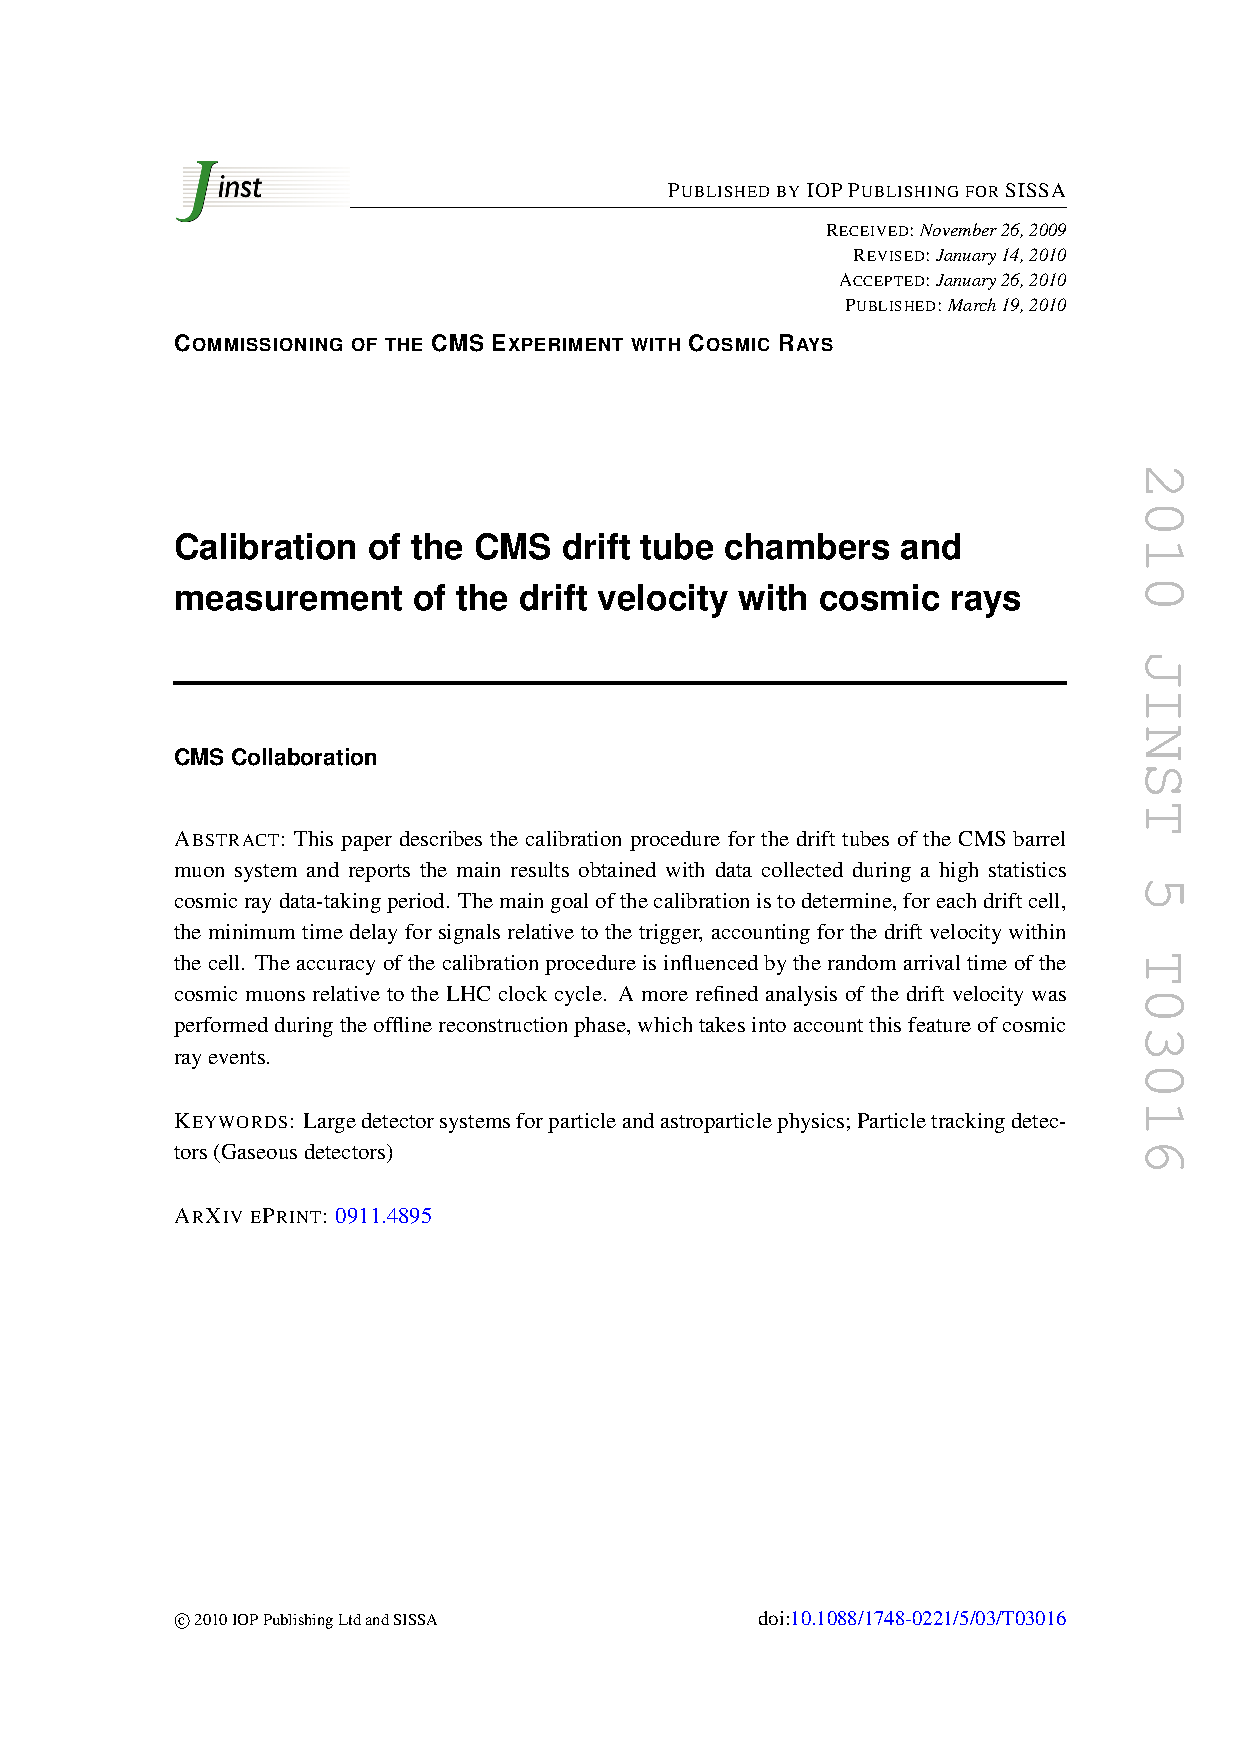
\includepdf[pages={1,2,3}]{Articulos/ArticulosReducidos/Investigacion_Publicaciones_CALIBRATION_OF_THE_CMS_DRIFT_TUBE_CHAMBERS_AND_MEASUREMENT_OF_THE.pdf}
\subsubsection{COMMISSIONING OF THE CMS EXPERIMENT AND THE COSMIC RUN AT FOUR TESLA}
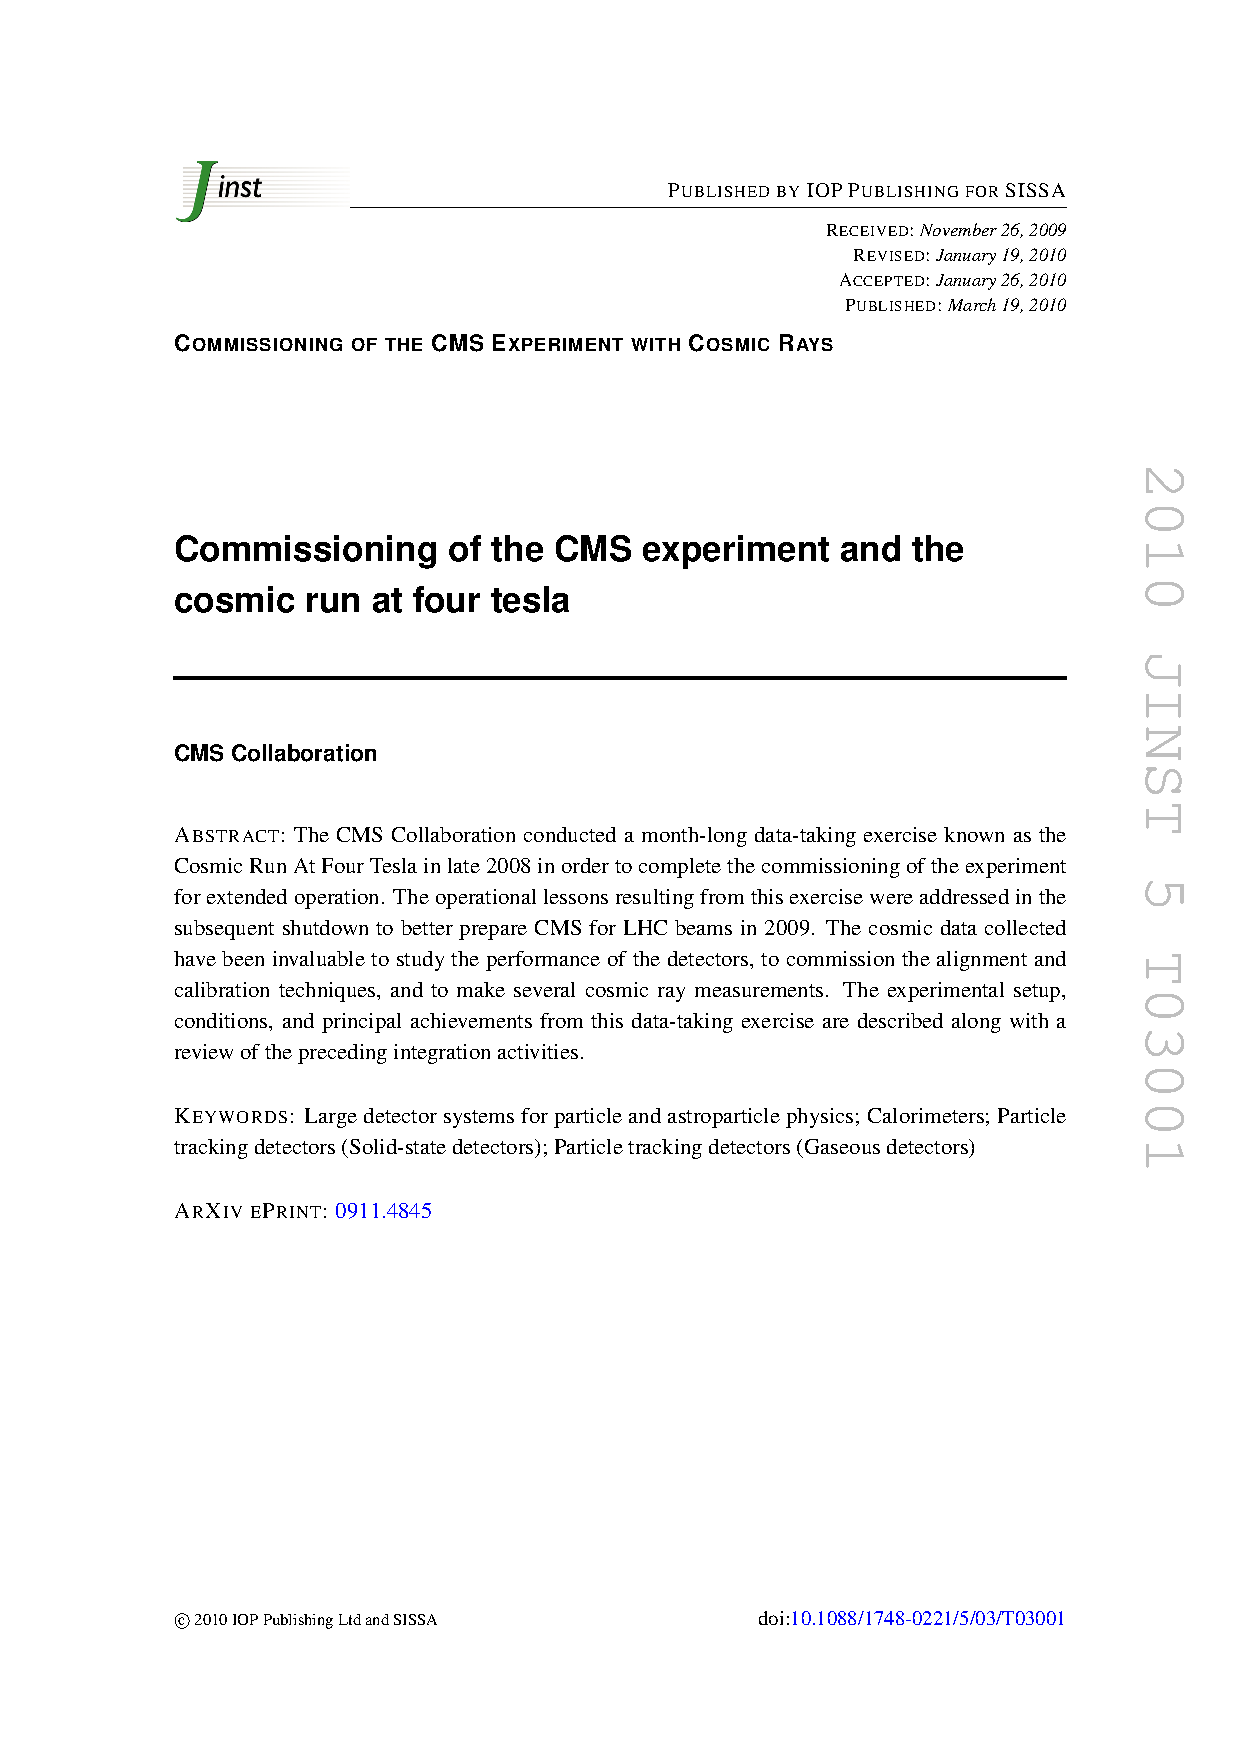
\includepdf[pages={1,2,3}]{Articulos/ArticulosReducidos/Investigacion_Publicaciones_COMMISSIONING_OF_THE_CMS_EXPERIMENT_AND_THE_COSMIC_RUN_AT_FOUR_TE.pdf}
\subsubsection{PERFORMANCE OF CMS MUON RECONSTRUCTION IN COSMIC-RAY EVENTS}
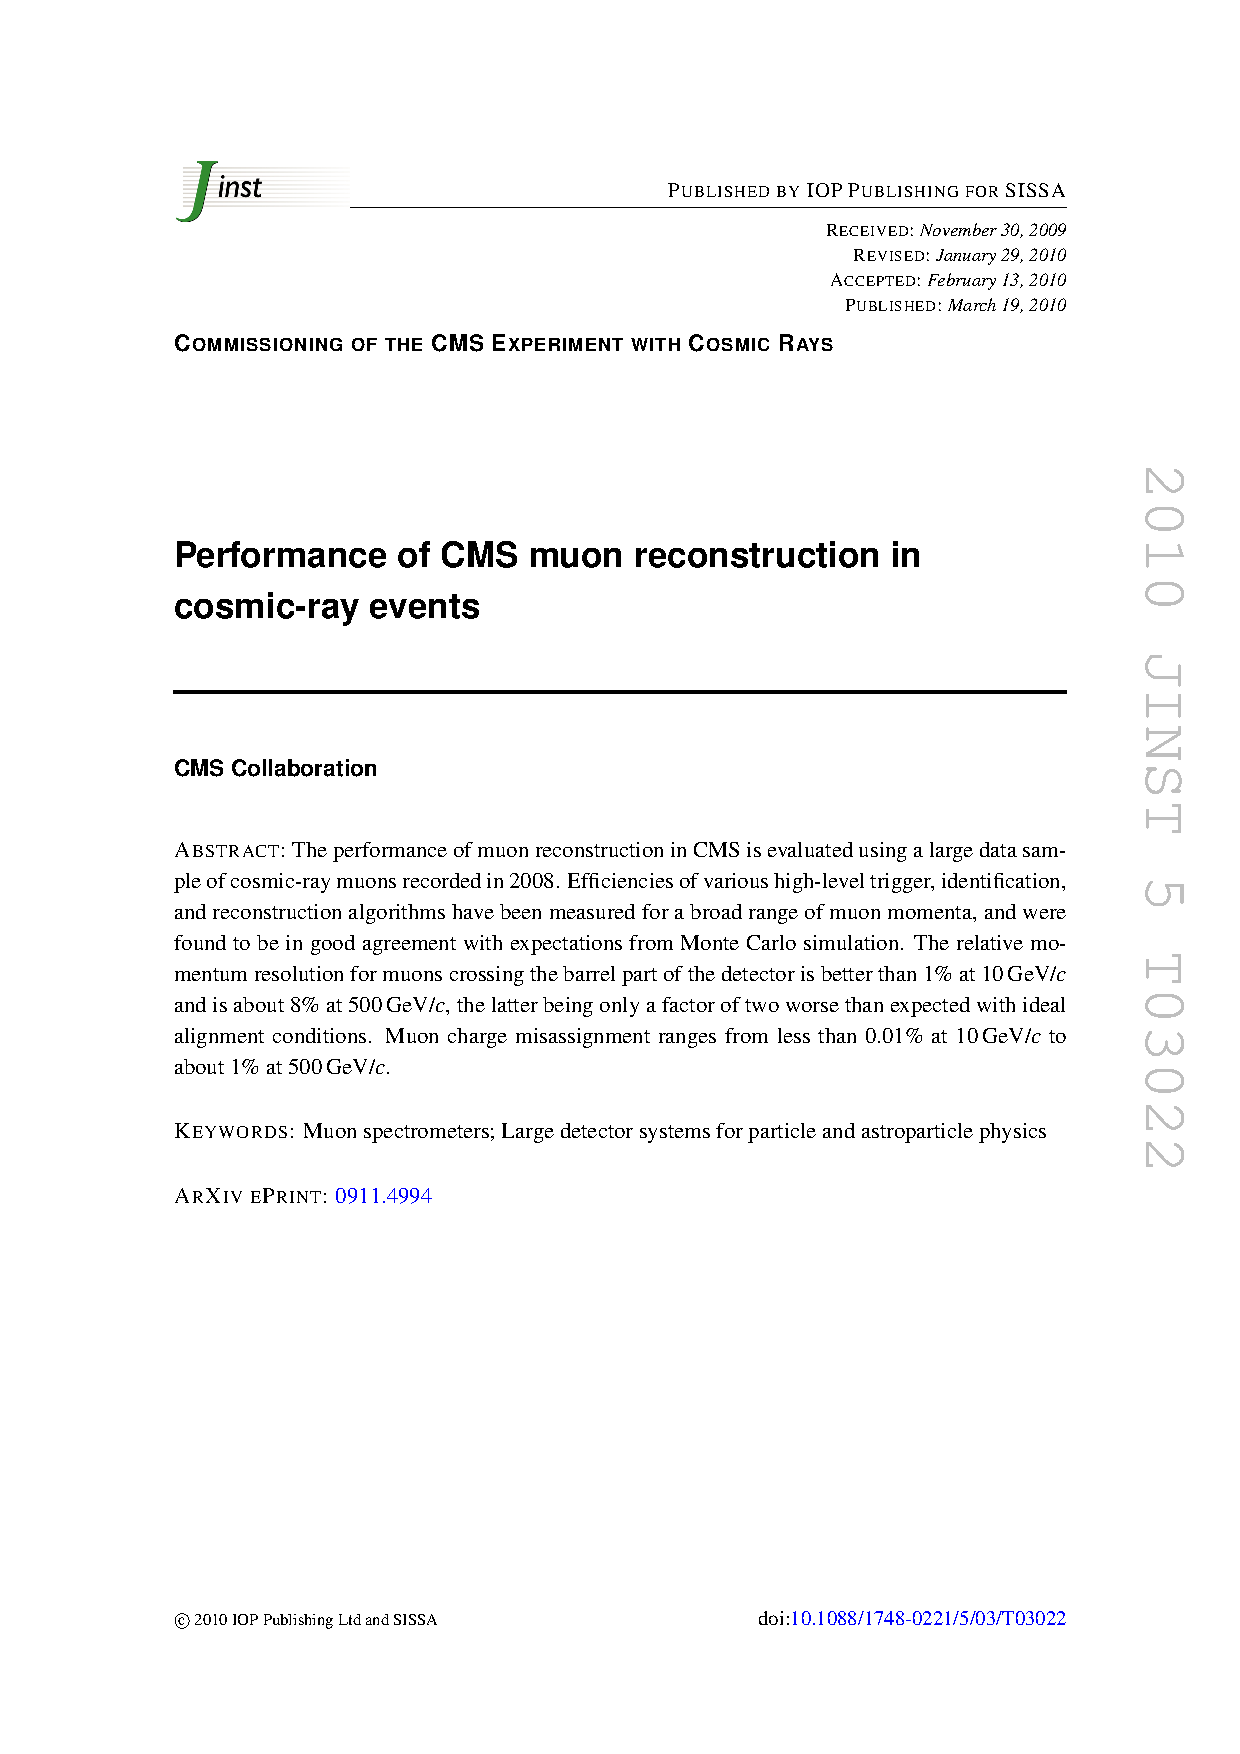
\includepdf[pages={1,2,3}]{Articulos/ArticulosReducidos/Investigacion_Publicaciones_PERFORMANCE_OF_CMS_MUON_RECONSTRUCTION_IN_COSMIC-RAY_EVENTS.pdf}
\subsubsection{PERFORMANCE OF THE CMS DRIFT TUBE CHAMBERS WITH COSMIC RAYS}
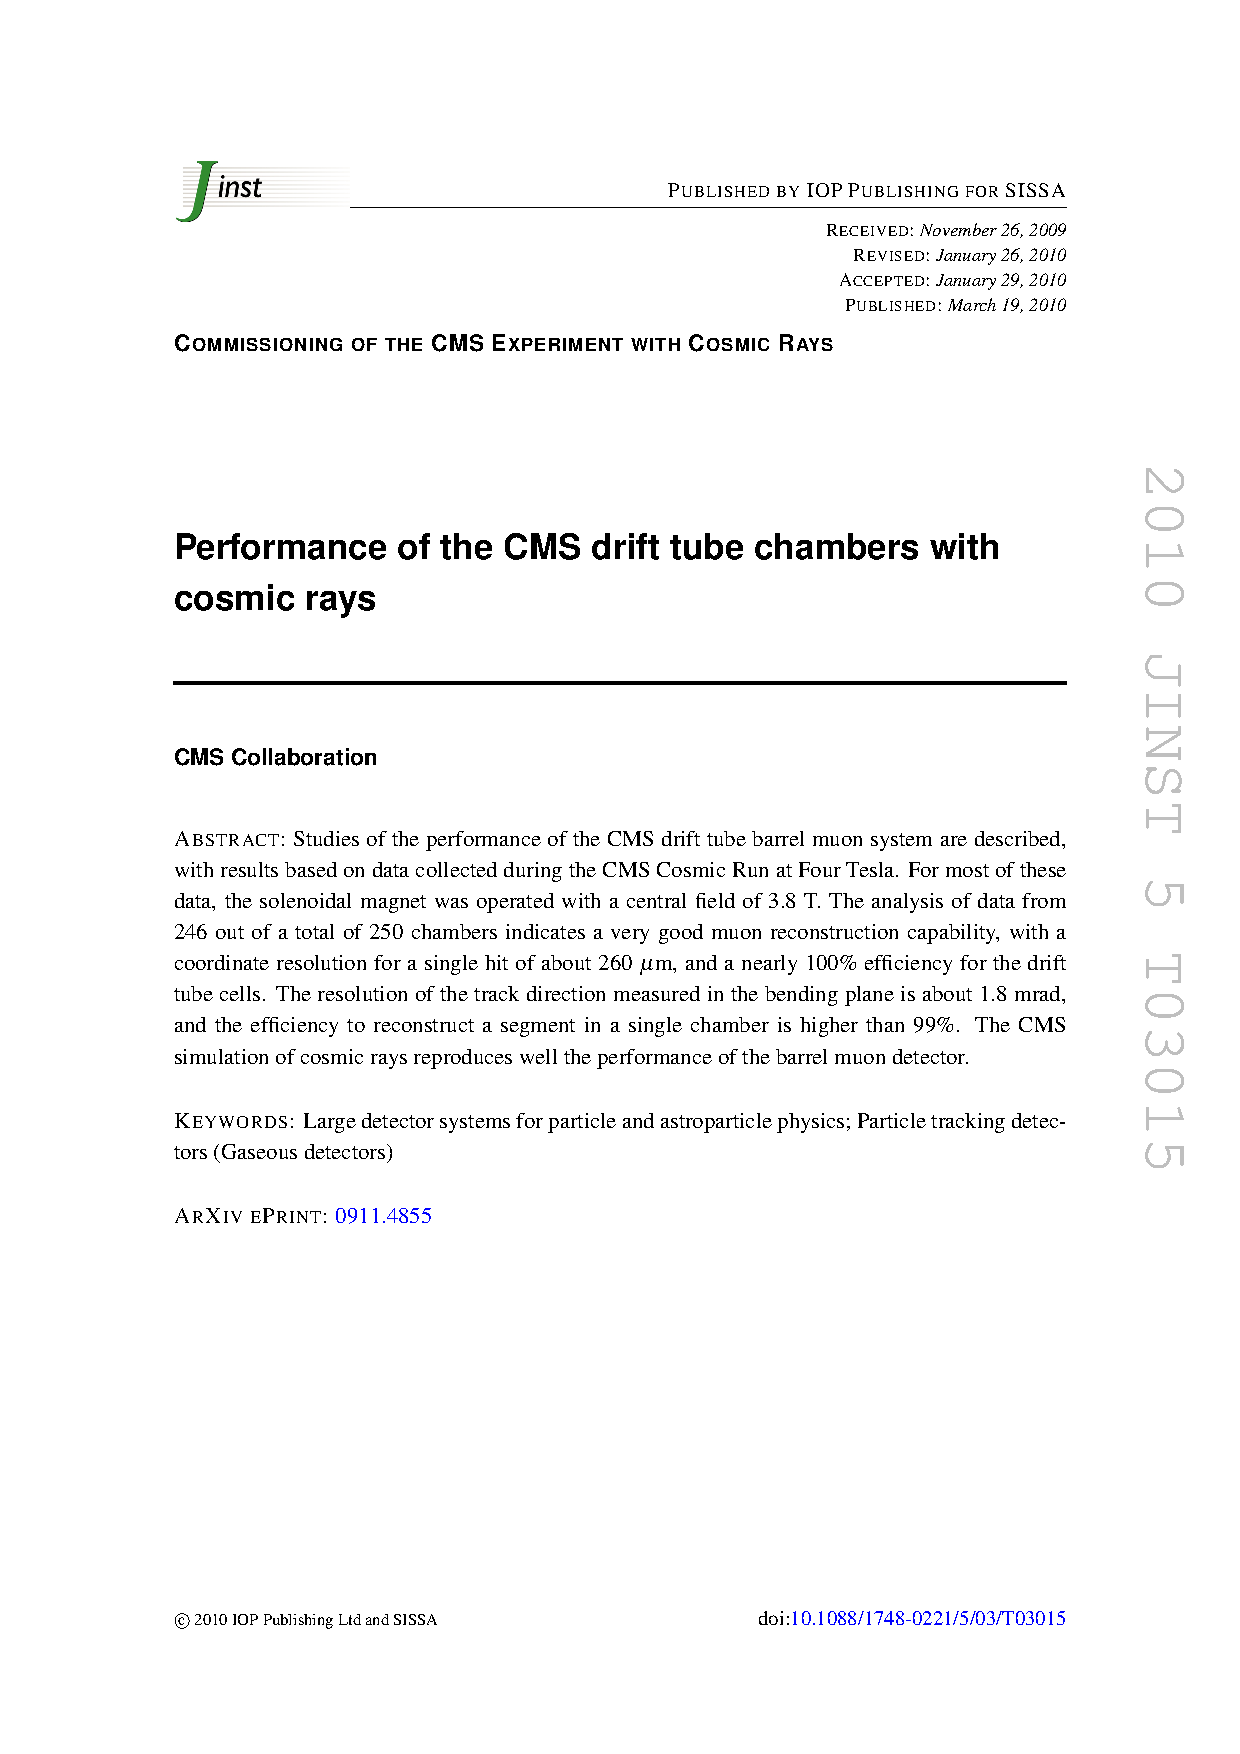
\includepdf[pages={1,2,3}]{Articulos/ArticulosReducidos/Investigacion_Publicaciones_PERFORMANCE_OF_THE_CMS_DRIFT_TUBE_CHAMBERS_WITH_COSMIC_RAYS.pdf}
\subsubsection{PRECISE MAPPING OF THE MAGNETIC FIELD IN THE CMS BARREL YOKE USING COSMIC RAYS}
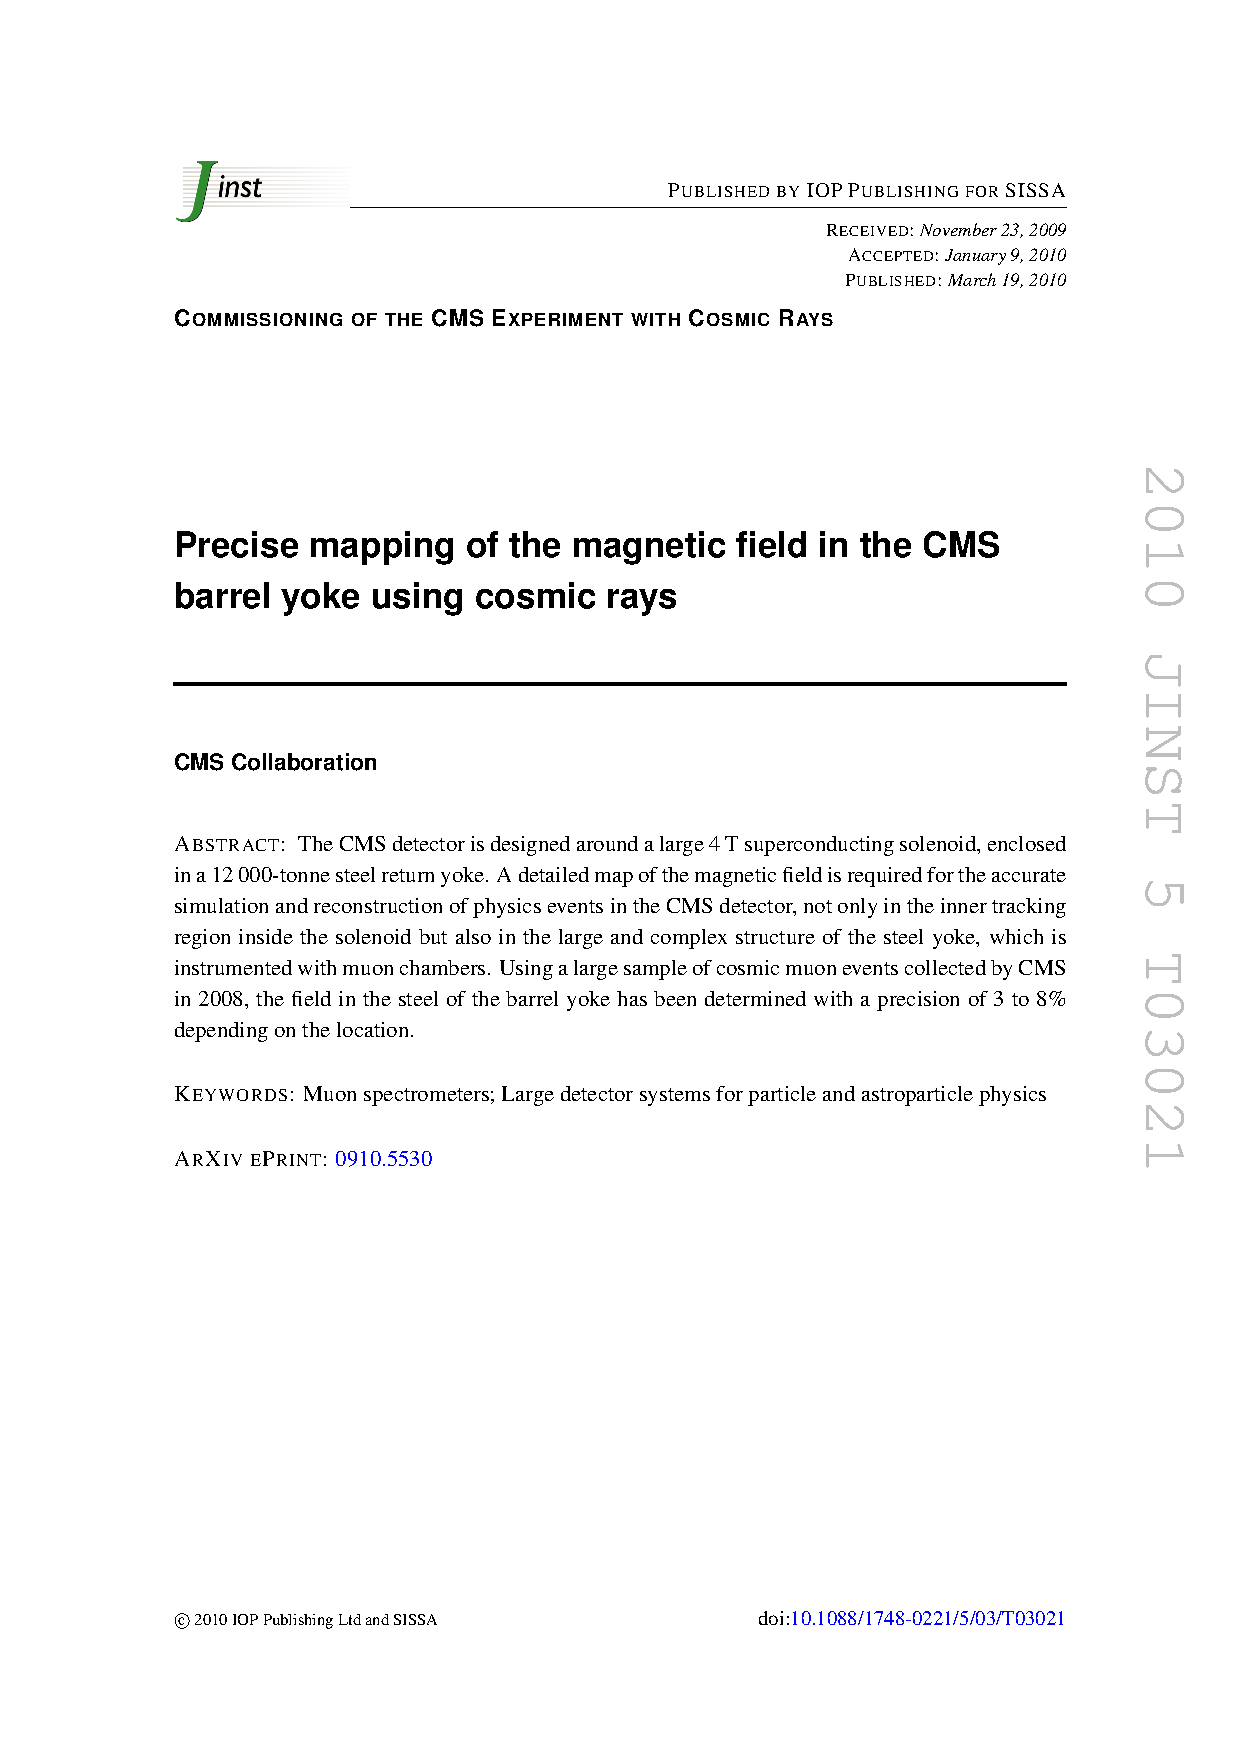
\includepdf[pages={1,2,3}]{Articulos/ArticulosReducidos/Investigacion_Publicaciones_PRECISE_MAPPING_OF_THE_MAGNETIC_FIELD_IN_THE_CMS_BARREL_YOKE_USIN.pdf}
\subsubsection{MEASUREMENT OF THE CHARGE RATIO OF ATMOSPHERIC MUONS WITH THE CMS DETECTOR}
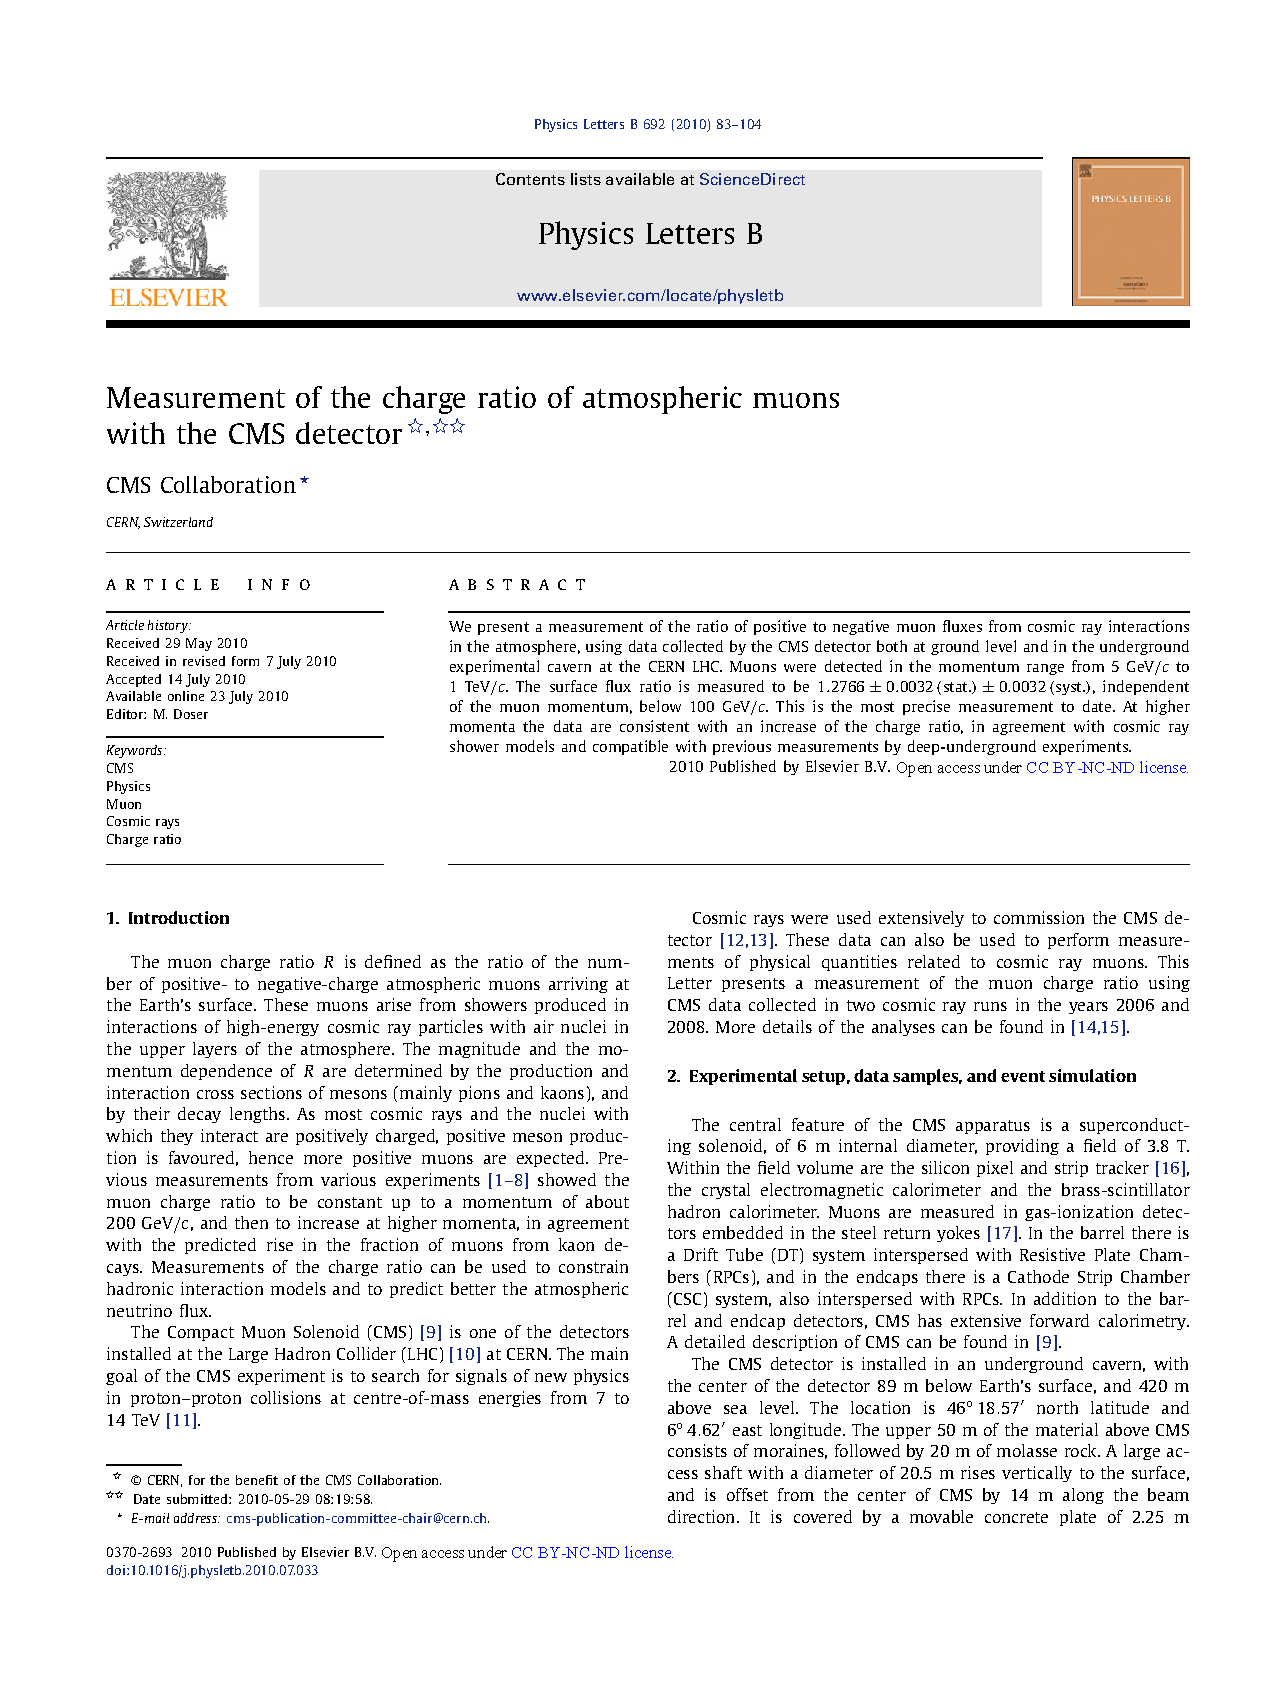
\includepdf[pages={1,2,3}]{Articulos/ArticulosReducidos/Investigacion_Publicaciones_MEASUREMENT_OF_THE_CHARGE_RATIO_OF_ATMOSPHERIC_MUONS_WITH_THE_CMS.pdf}
\subsubsection{SEARCH FOR PHYSICS BEYOND THE STANDARD MODEL IN OPPOSITE-SIGN DILEPTON EVENTS IN PP COLLISIONS AT SQRT S 7 TEV}
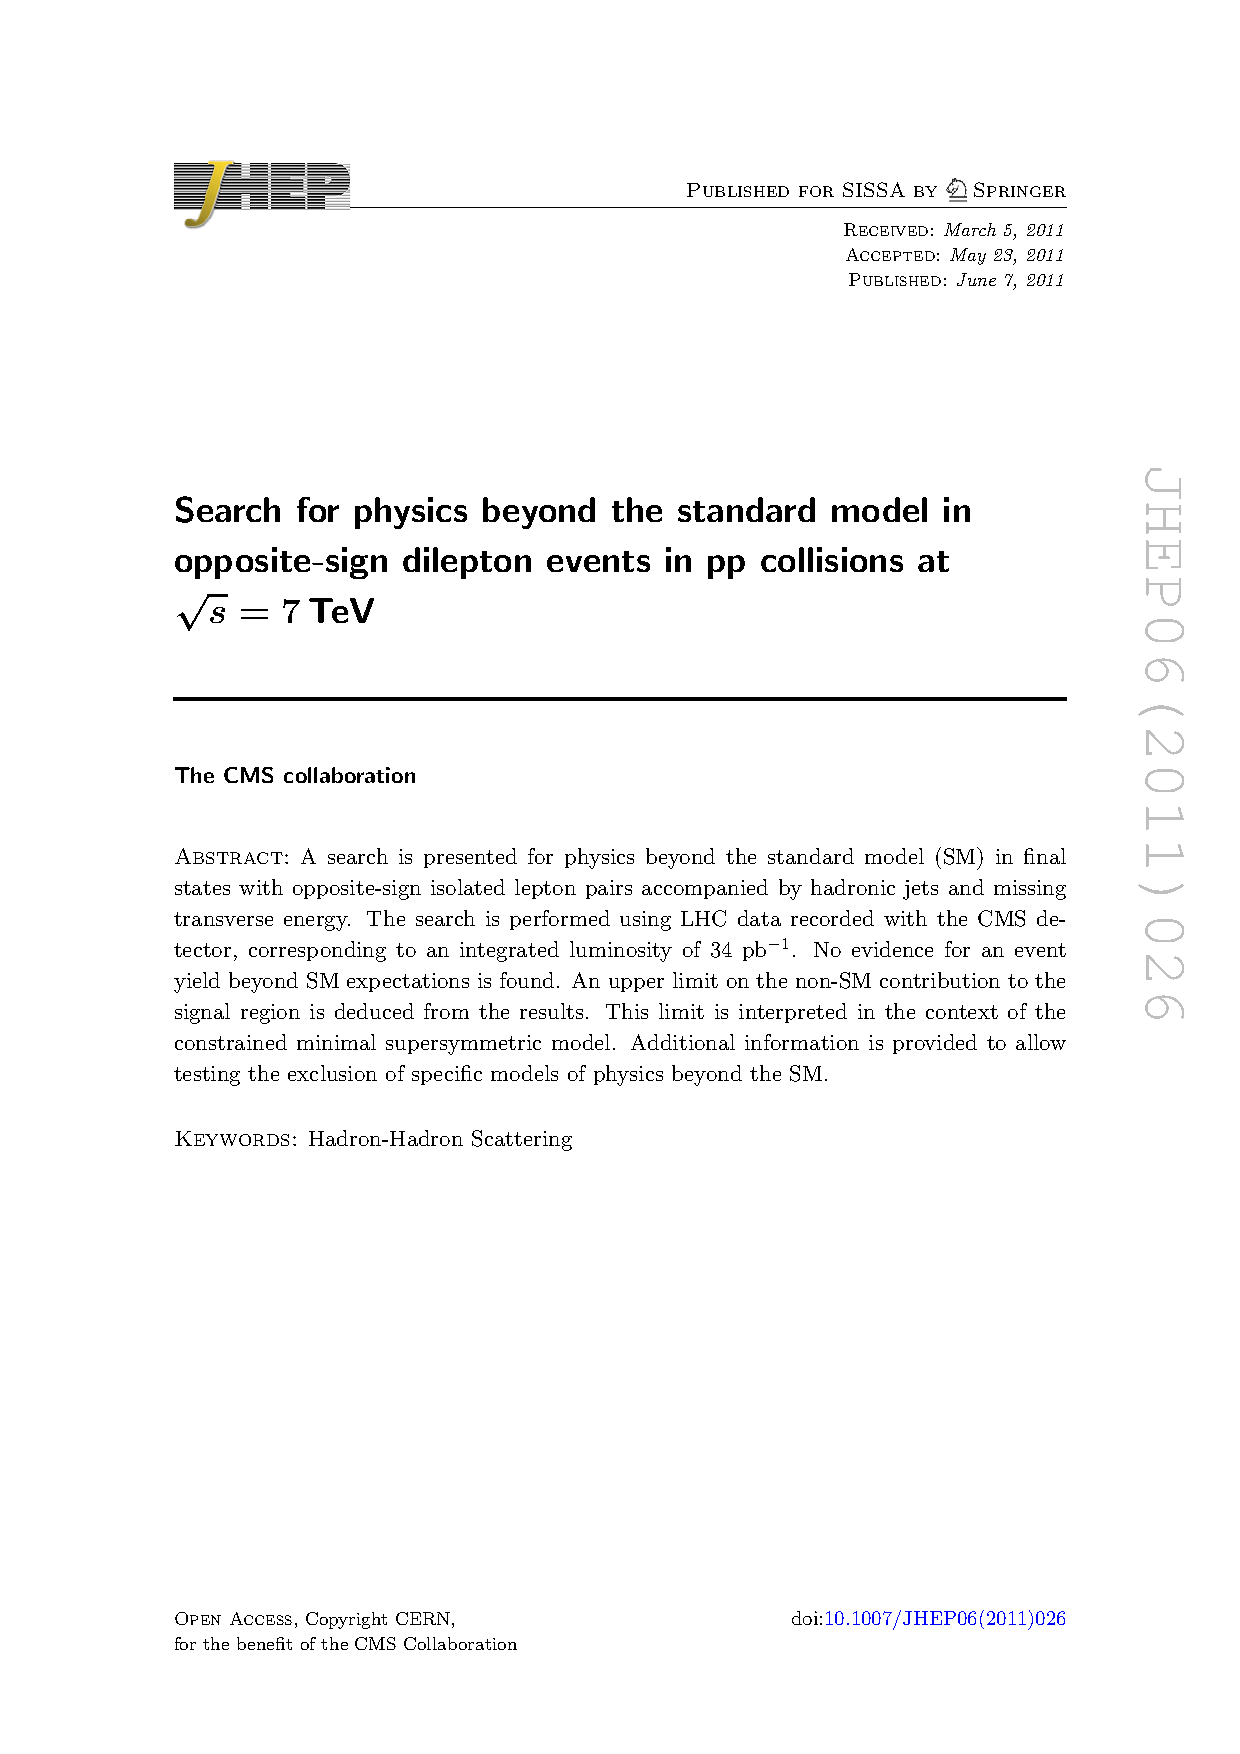
\includepdf[pages={1,2,3}]{Articulos/ArticulosReducidos/Investigacion_Publicaciones_SEARCH_FOR_PHYSICS_BEYOND_THE_STANDARD_MODEL_IN_OPPOSITE-SIGN_DIL.pdf}
\subsubsection{Search for new physics with same-sign isolated dilepton events with jets and missing transverse energy at the LHC}
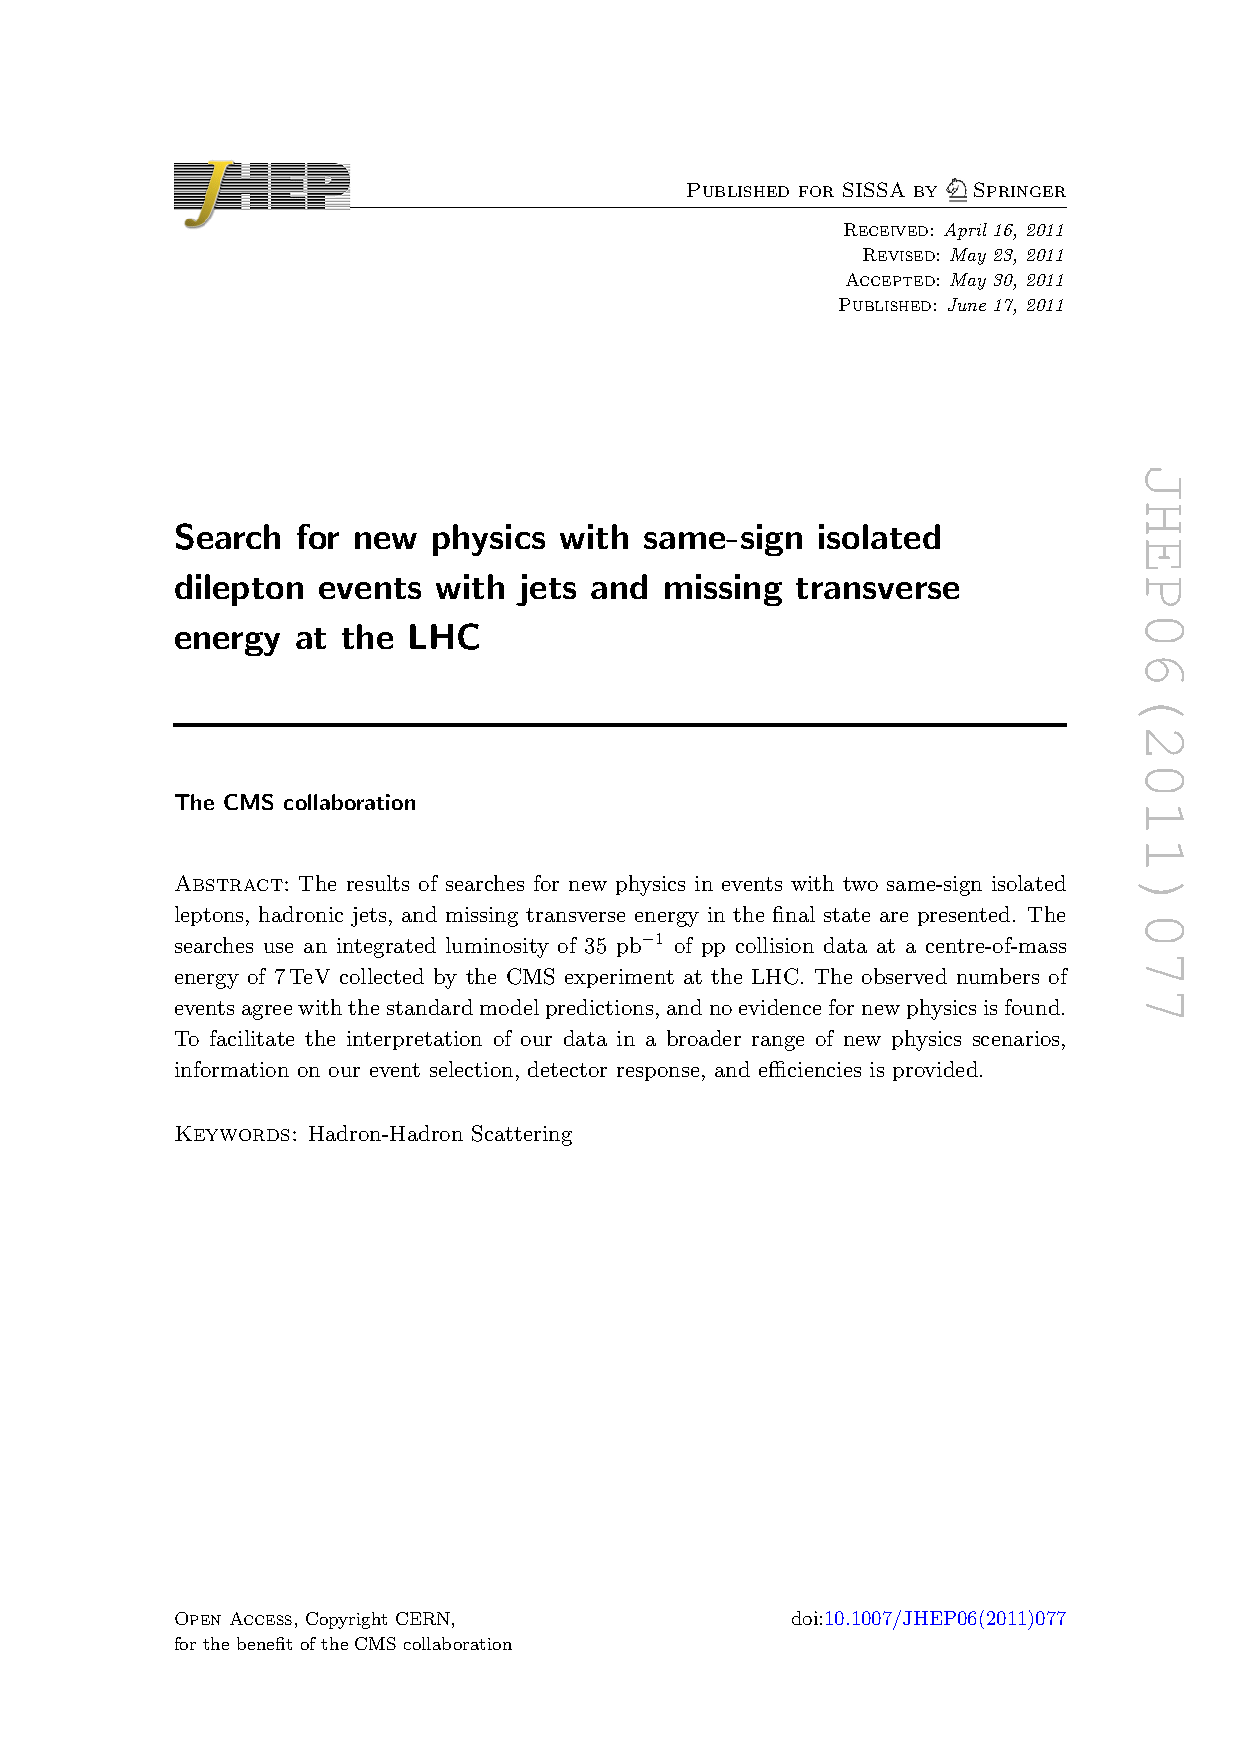
\includepdf[pages={1,2,3}]{Articulos/ArticulosReducidos/Investigacion_Publicaciones_Search_For_New_Physics_With_Same_Sign_Isolated_Dolepton_Events_With_Jets_And_Missing.pdf}
\subsubsection{SEARCH FOR NEW PHYSICS WITH SAME-SIGN ISOLATED DILEPTON EVENTS WITH JETS AND MISSING TRANSVERSE ENERGY}
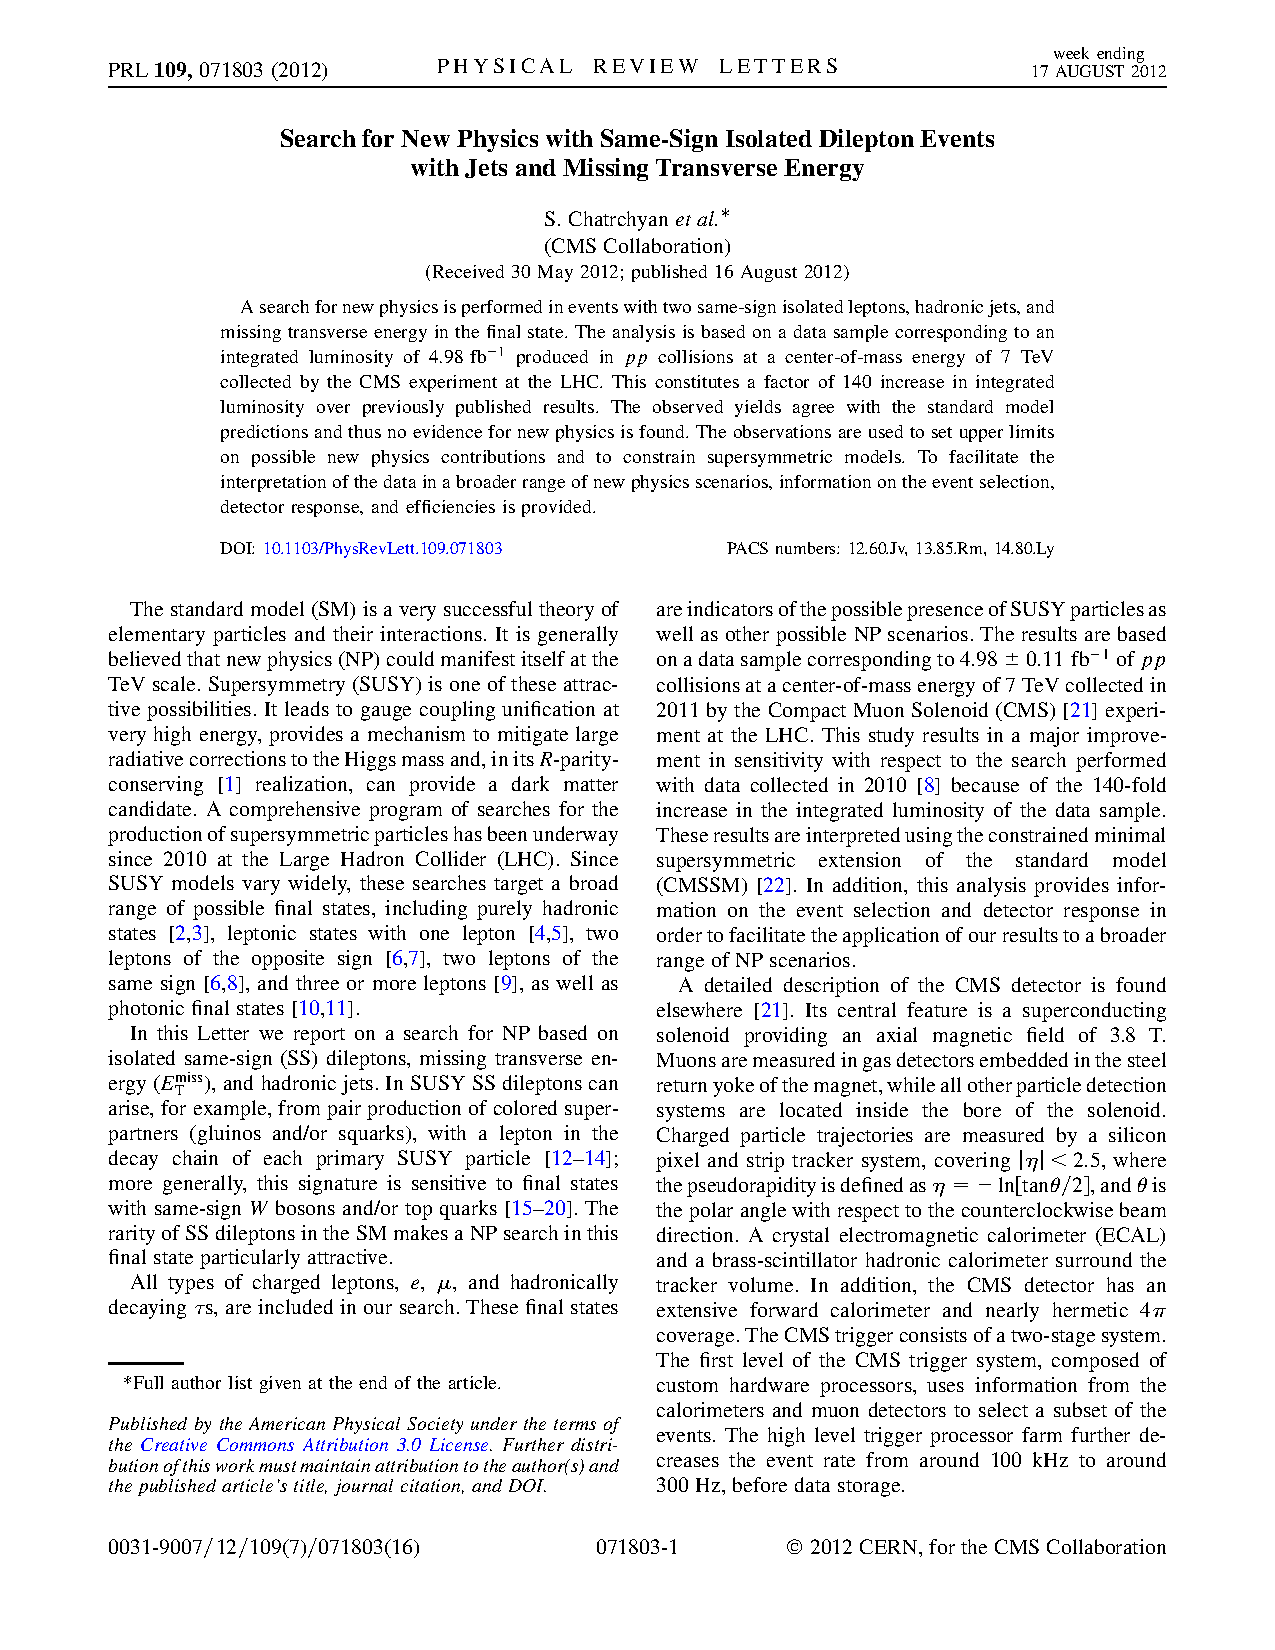
\includepdf[pages={1,2,3}]{Articulos/ArticulosReducidos/Investigacion_Publicaciones_SEARCH_FOR_NEW_PHYSICS_WITH_SAME-SIGN_ISOLATED_DILEPTON_EVENTS_WI.pdf}
\subsubsection{SEARCH FOR SUPERSYMMETRY IN HADRONIC FINAL STATES USING MT2 IN PP COLLISIONS AT 7 TEV}
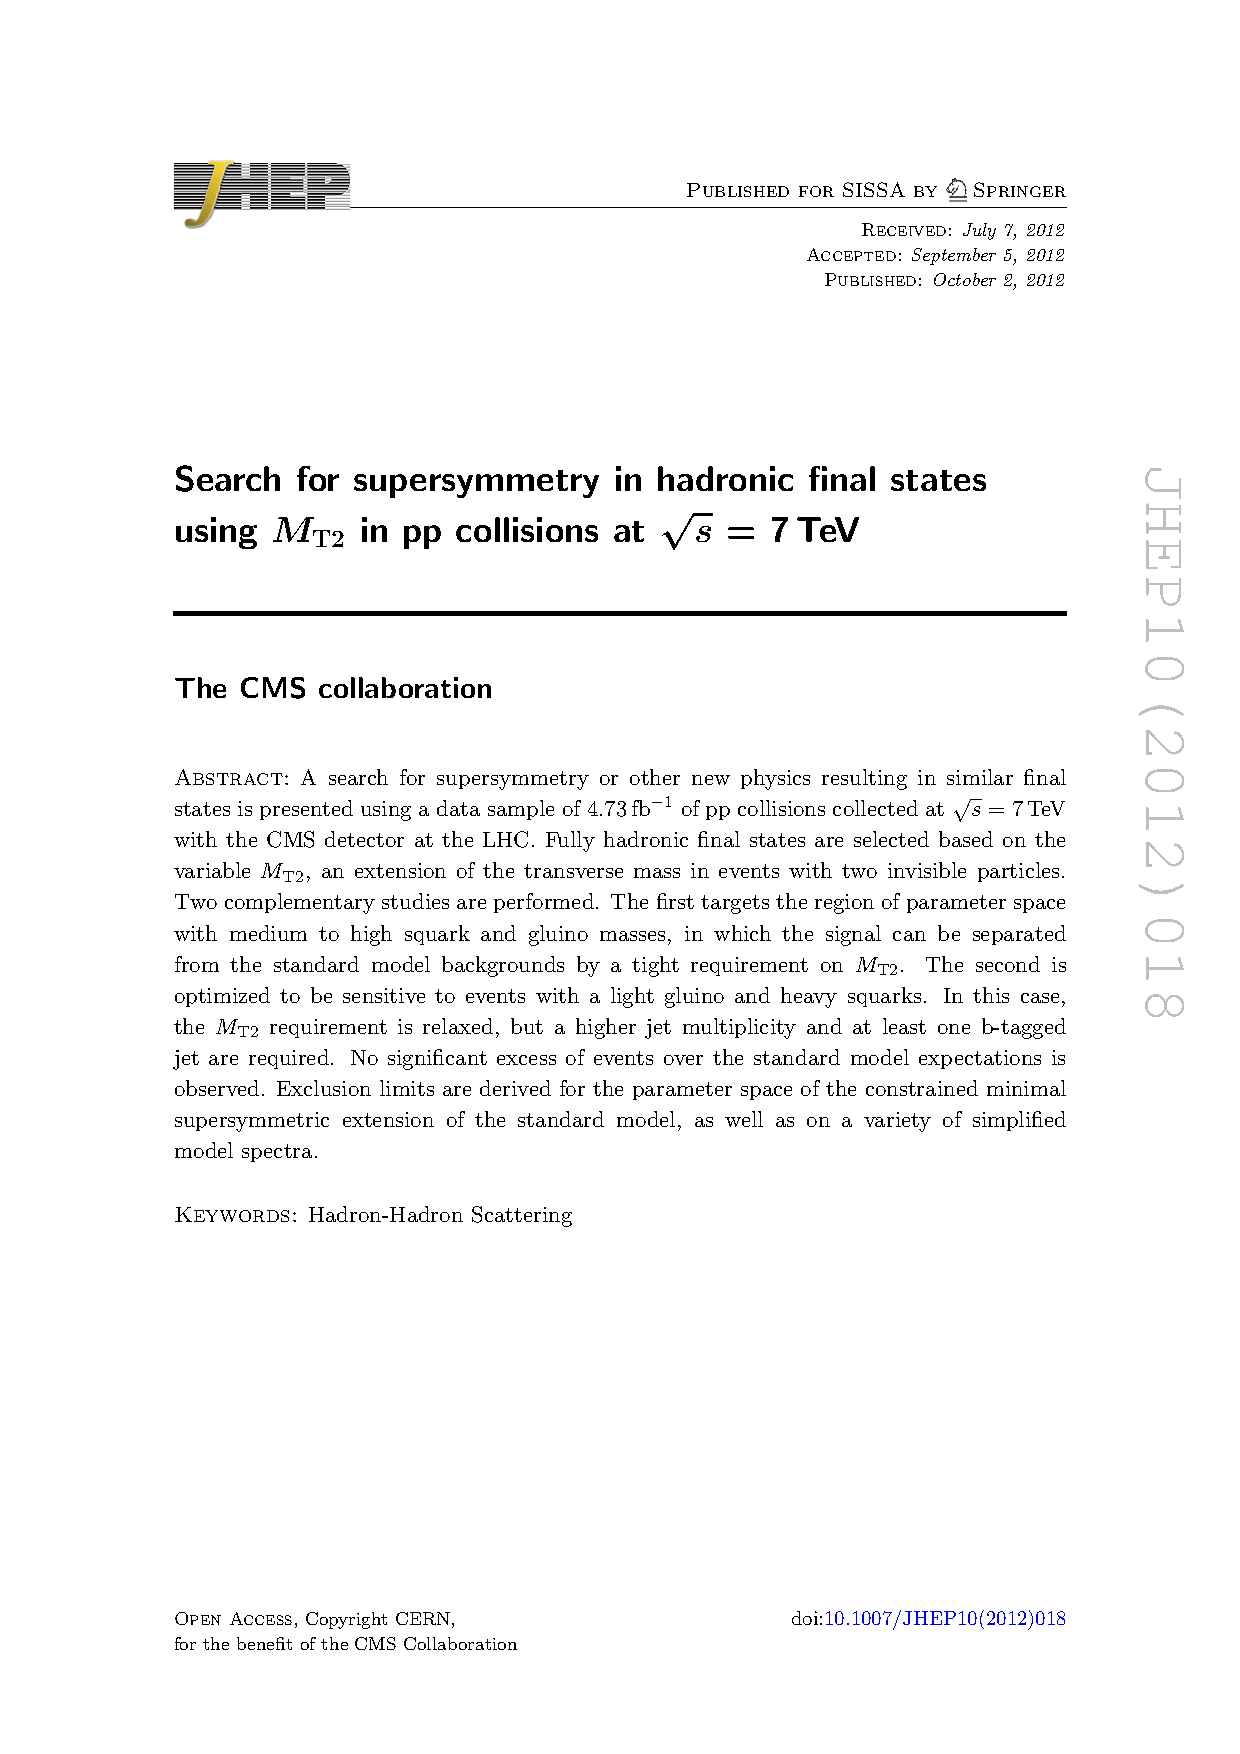
\includepdf[pages={1,2,3}]{Articulos/ArticulosReducidos/Investigacion_Publicaciones_SEARCH_FOR_SUPERSYMMETRY_IN_HADRONIC_FINAL_STATES_USING_MT2_IN_PP.pdf}
\subsubsection{SEARCH FOR PHYSICS BEYOND THE STANDARD MODEL IN EVENTS WITH A Z BOSON JETS AND MISSING TRANSVERSE ENERGY}
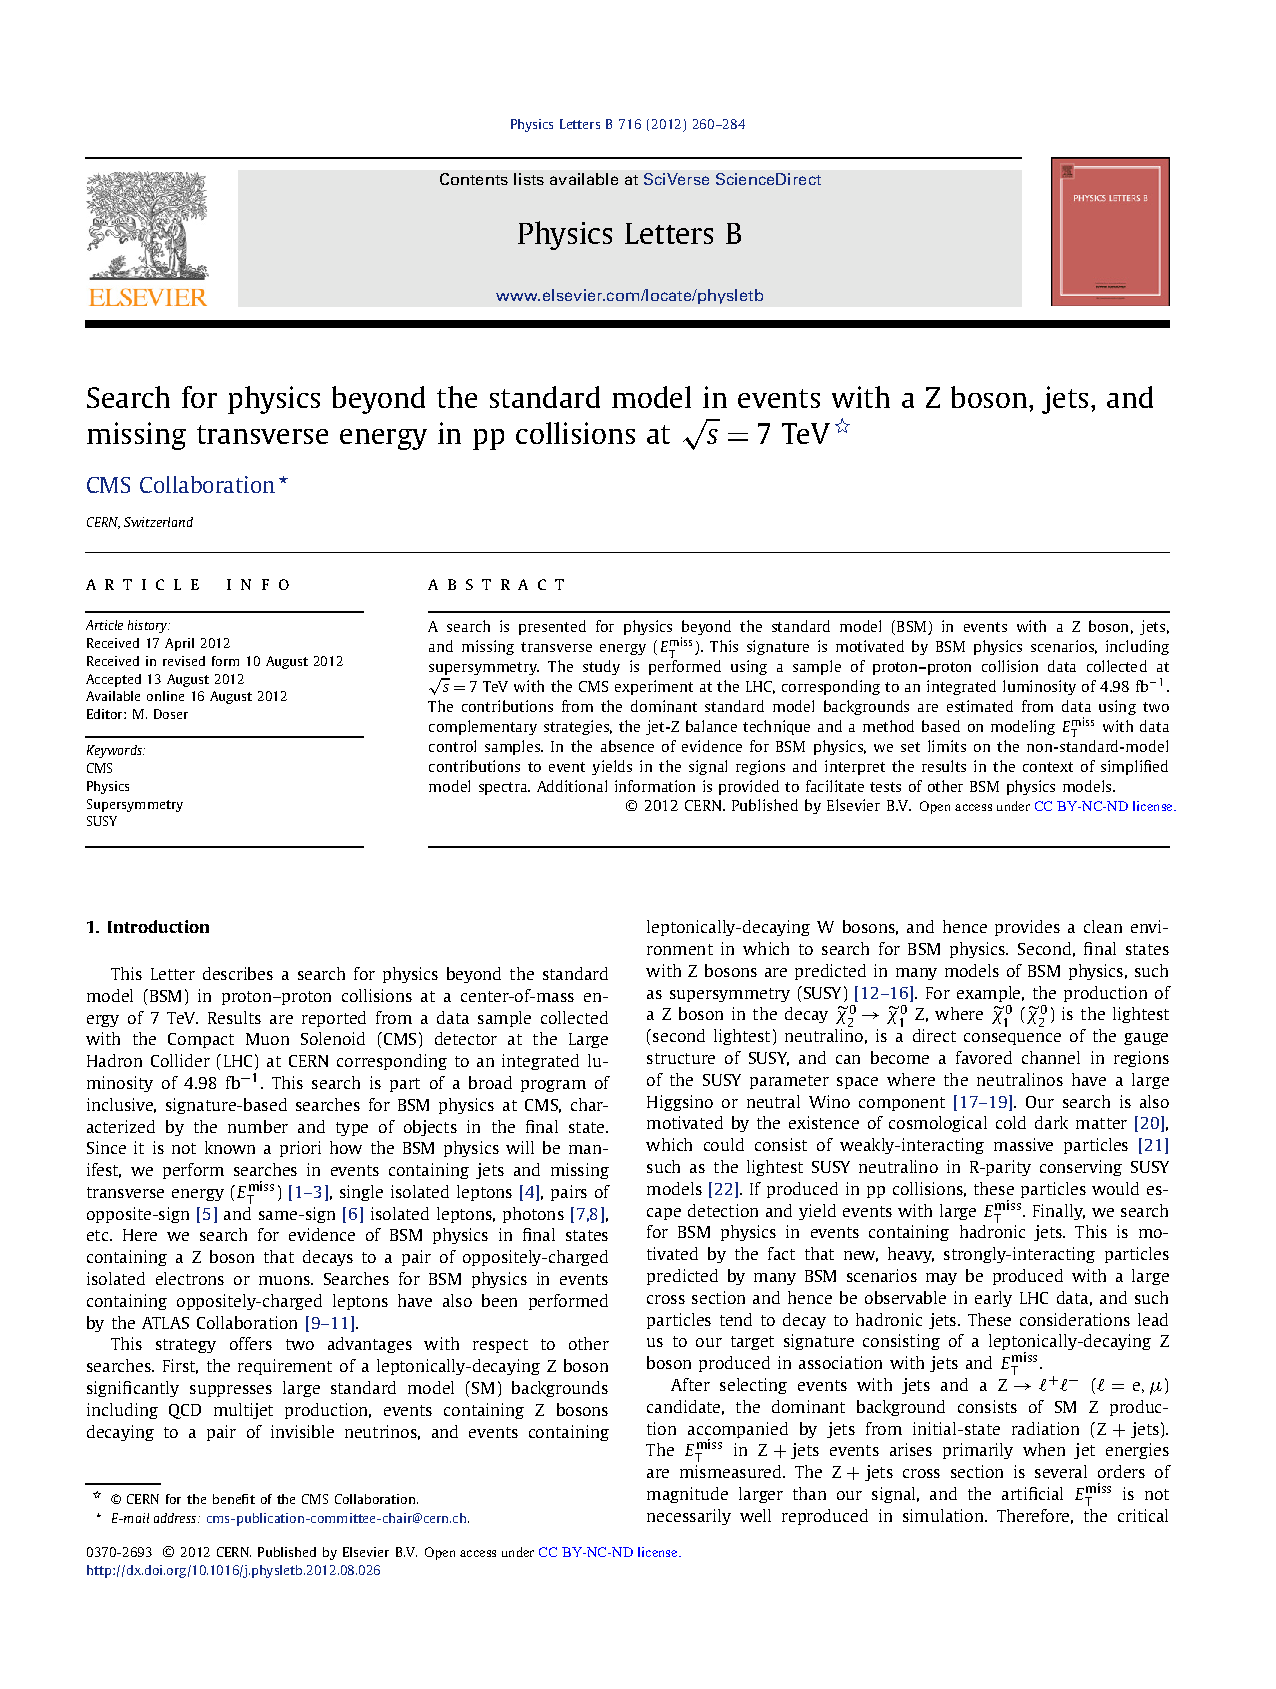
\includepdf[pages={1,2,3}]{Articulos/ArticulosReducidos/Investigacion_Publicaciones_SEARCH_FOR_PHYSICS_BEYOND_THE_STANDARD_MODEL_IN_EVENTS_WITH_A_Z_B.pdf}
\subsubsection{Search for new physics in events with same-sign dileptons and b-tagged jets in pp collisions at sqrt s 7 TeV}
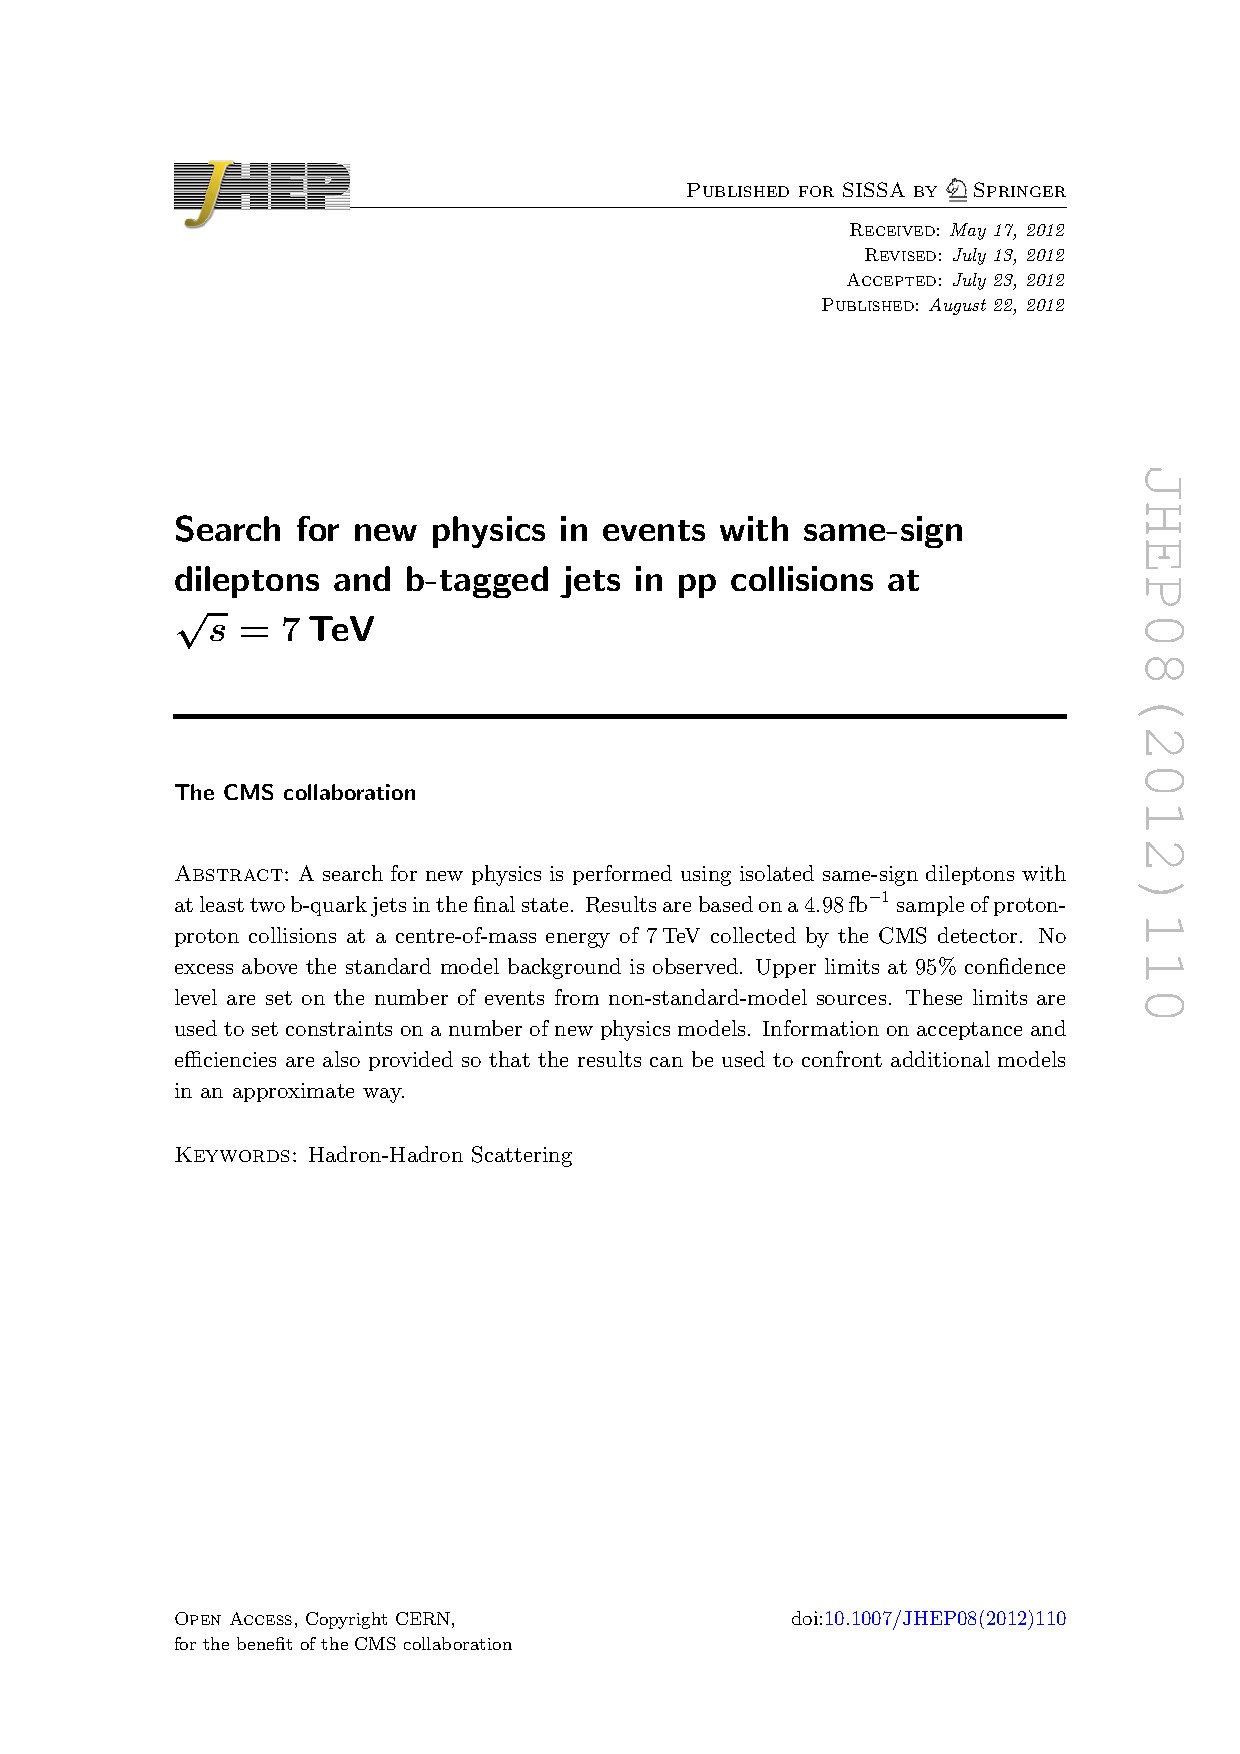
\includepdf[pages={1,2,3}]{Articulos/ArticulosReducidos/Investigacion_Publicaciones_Search_for_new_physics_in_events_with_same-sign_dileptons_and_b-t.pdf}
\subsubsection{Performance of CMS Muon Reconstruction in pp Collision Events at sqrt s 7 TeV}
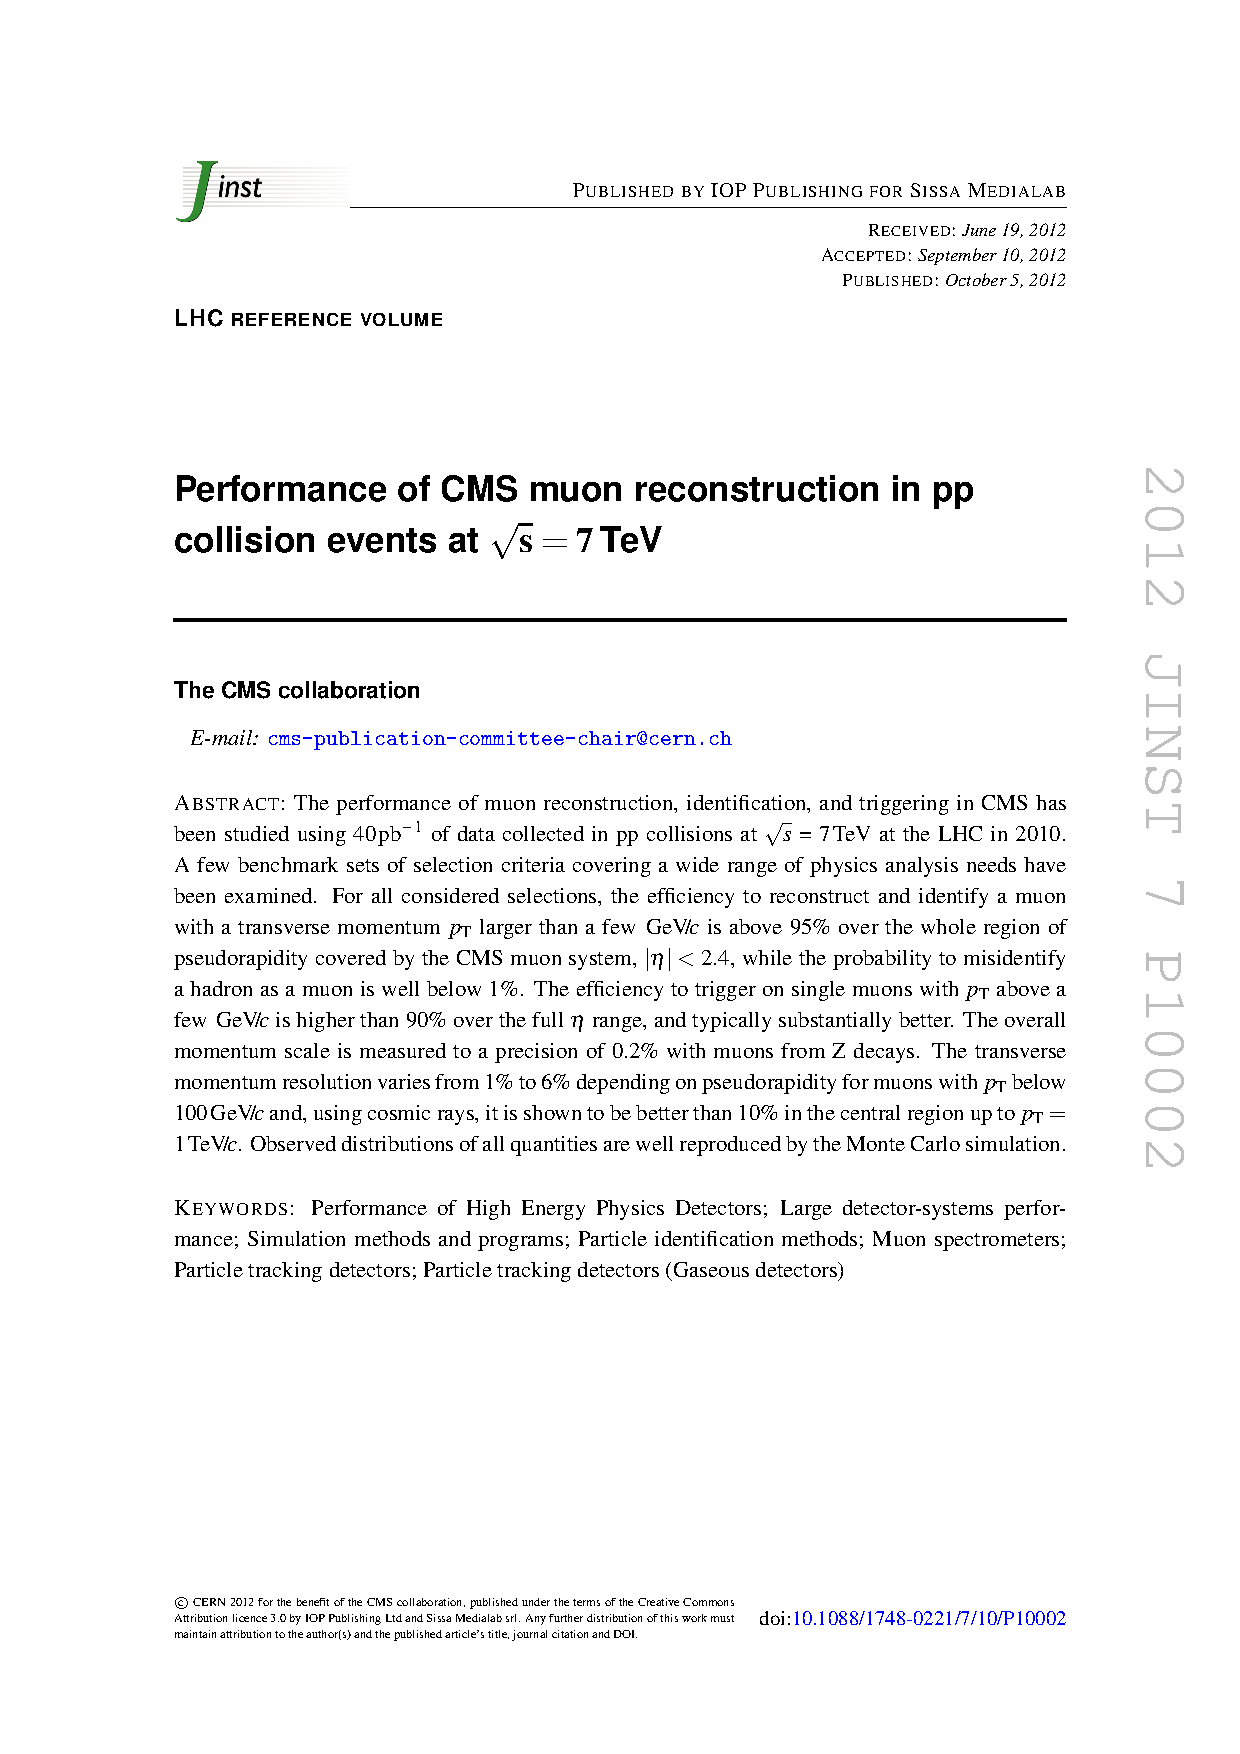
\includepdf[pages={1,2,3}]{Articulos/ArticulosReducidos/Investigacion_Publicaciones_Performance_of_CMS_Muon_Reconstruction_in_pp_Collision_Events_at_.pdf}
\subsubsection{INTERPRETATION OF SEARCHES FOR SUPERSYMMETRY WITH SIMPLIFIED MODELS}
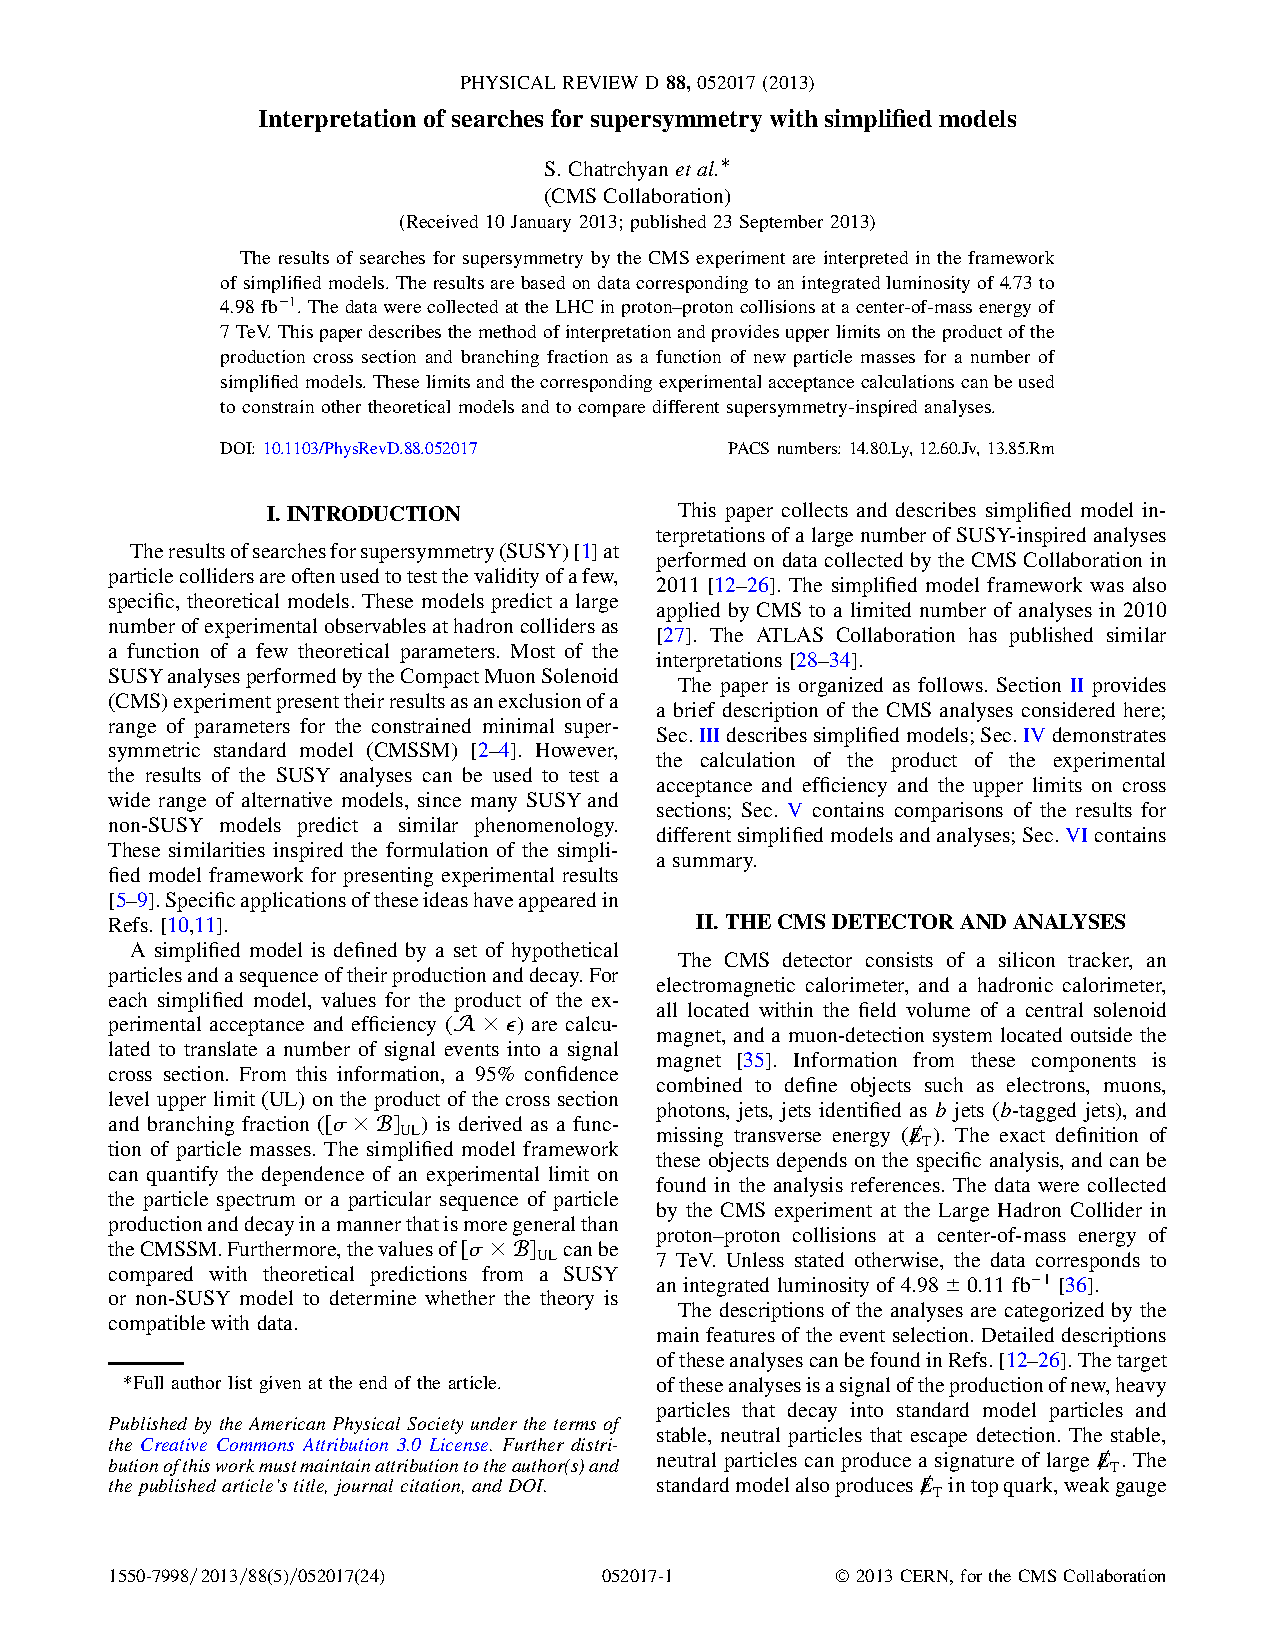
\includepdf[pages={1,2,3}]{Articulos/ArticulosReducidos/Investigacion_Publicaciones_INTERPRETATION_OF_SEARCHES_FOR_SUPERSYMMETRY_WITH_SIMPLIFIED_MODE.pdf}
\subsubsection{SEARCH FOR NEW PHYSICS IN EVENTS WITH OPPOSITE-SIGN LEPTONS JETS AND MISSING TRANSVERSE ENERGY in pp collisions at sqrt s 7 TeV}
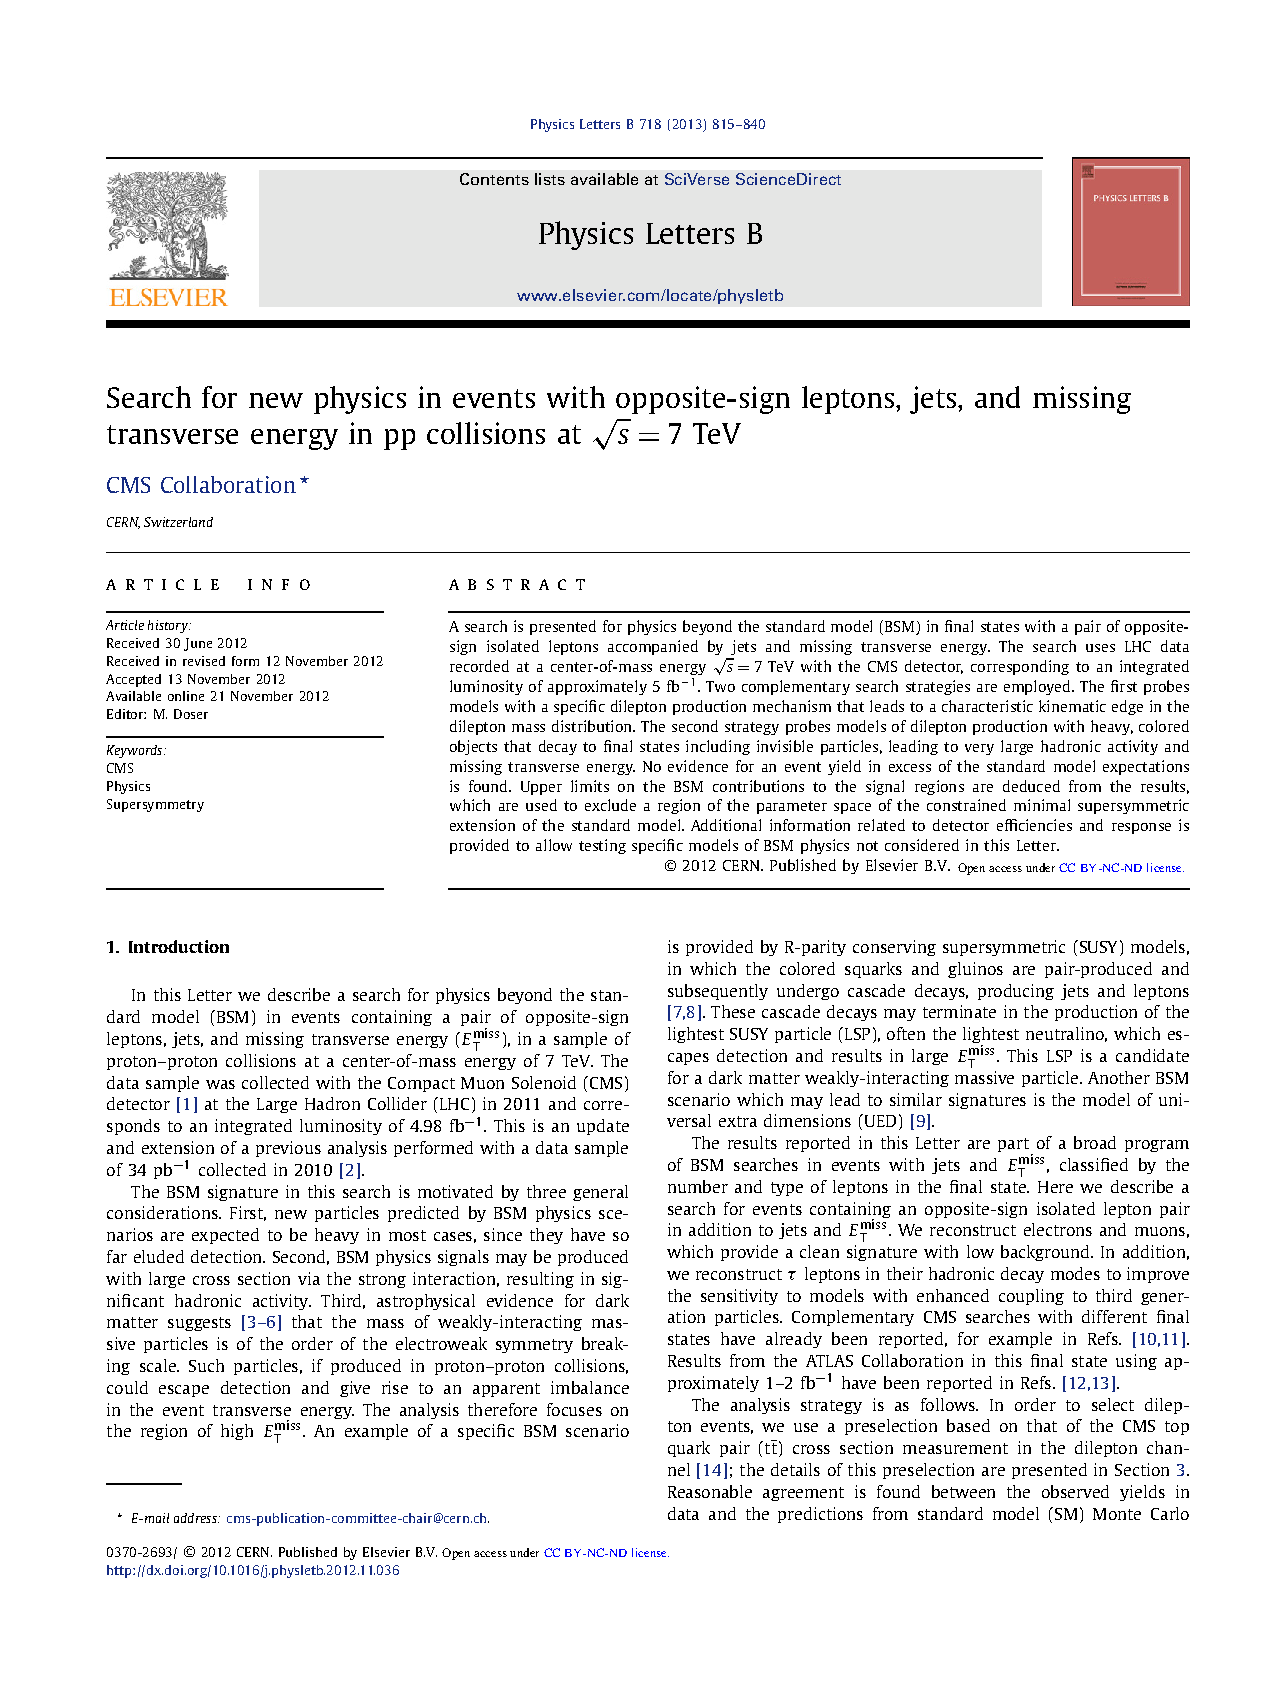
\includepdf[pages={1,2,3}]{Articulos/ArticulosReducidos/Investigacion_Publicaciones_SEARCH_FOR_NEW_PHYSICS_IN_EVENTS_WITH_OPPOSITE-SIGN_LEPTONS_JETS_.pdf}
\subsubsection{Search for Supersymmetry in Events with Opposite-Sign Dileptons and Missing Transverse Energy Using an Artificial Neural Network}
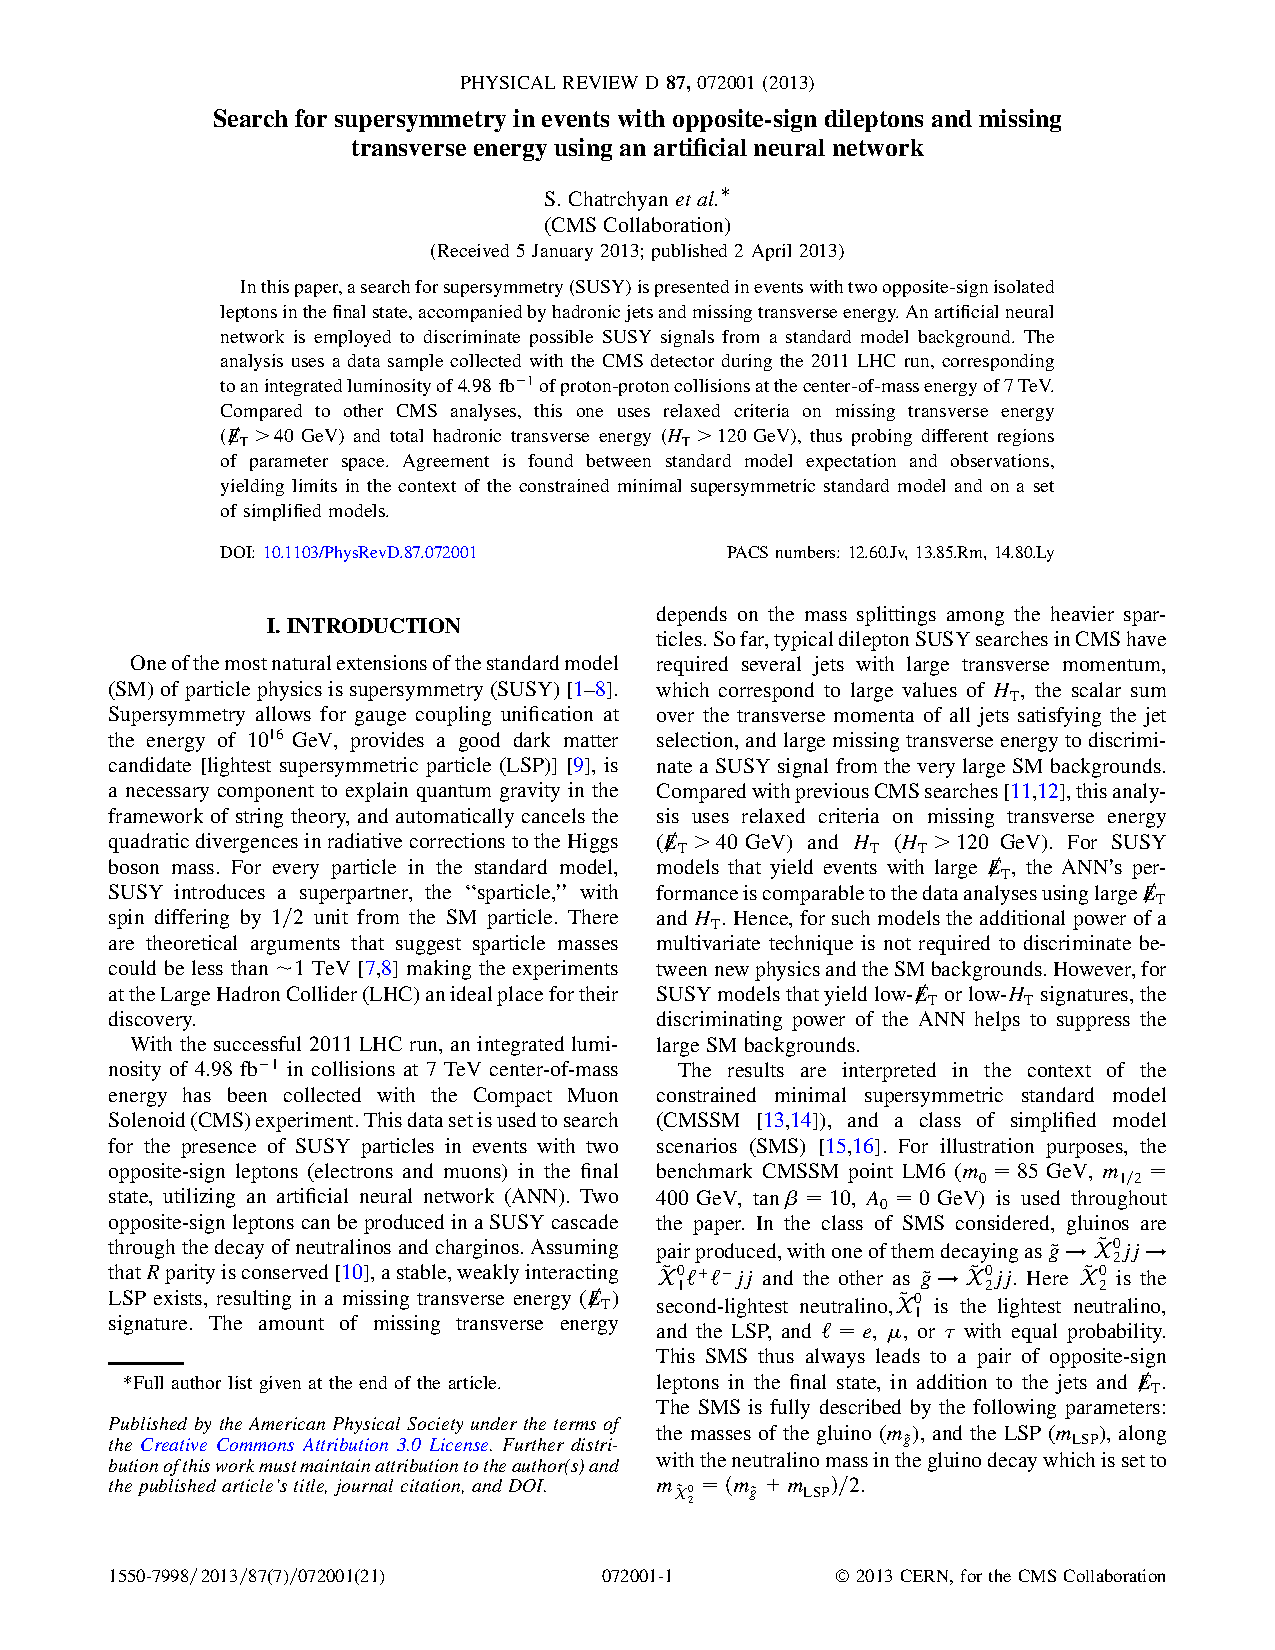
\includepdf[pages={1,2,3}]{Articulos/ArticulosReducidos/Investigacion_Publicaciones_Search_for_Supersymmetry_in_Events_with_Opposite-Sign_Dileptons_a.pdf}
\subsubsection{Search for new physics in events with same-sign dileptons and jets in pp collisions at sqrt s 8 TeV}
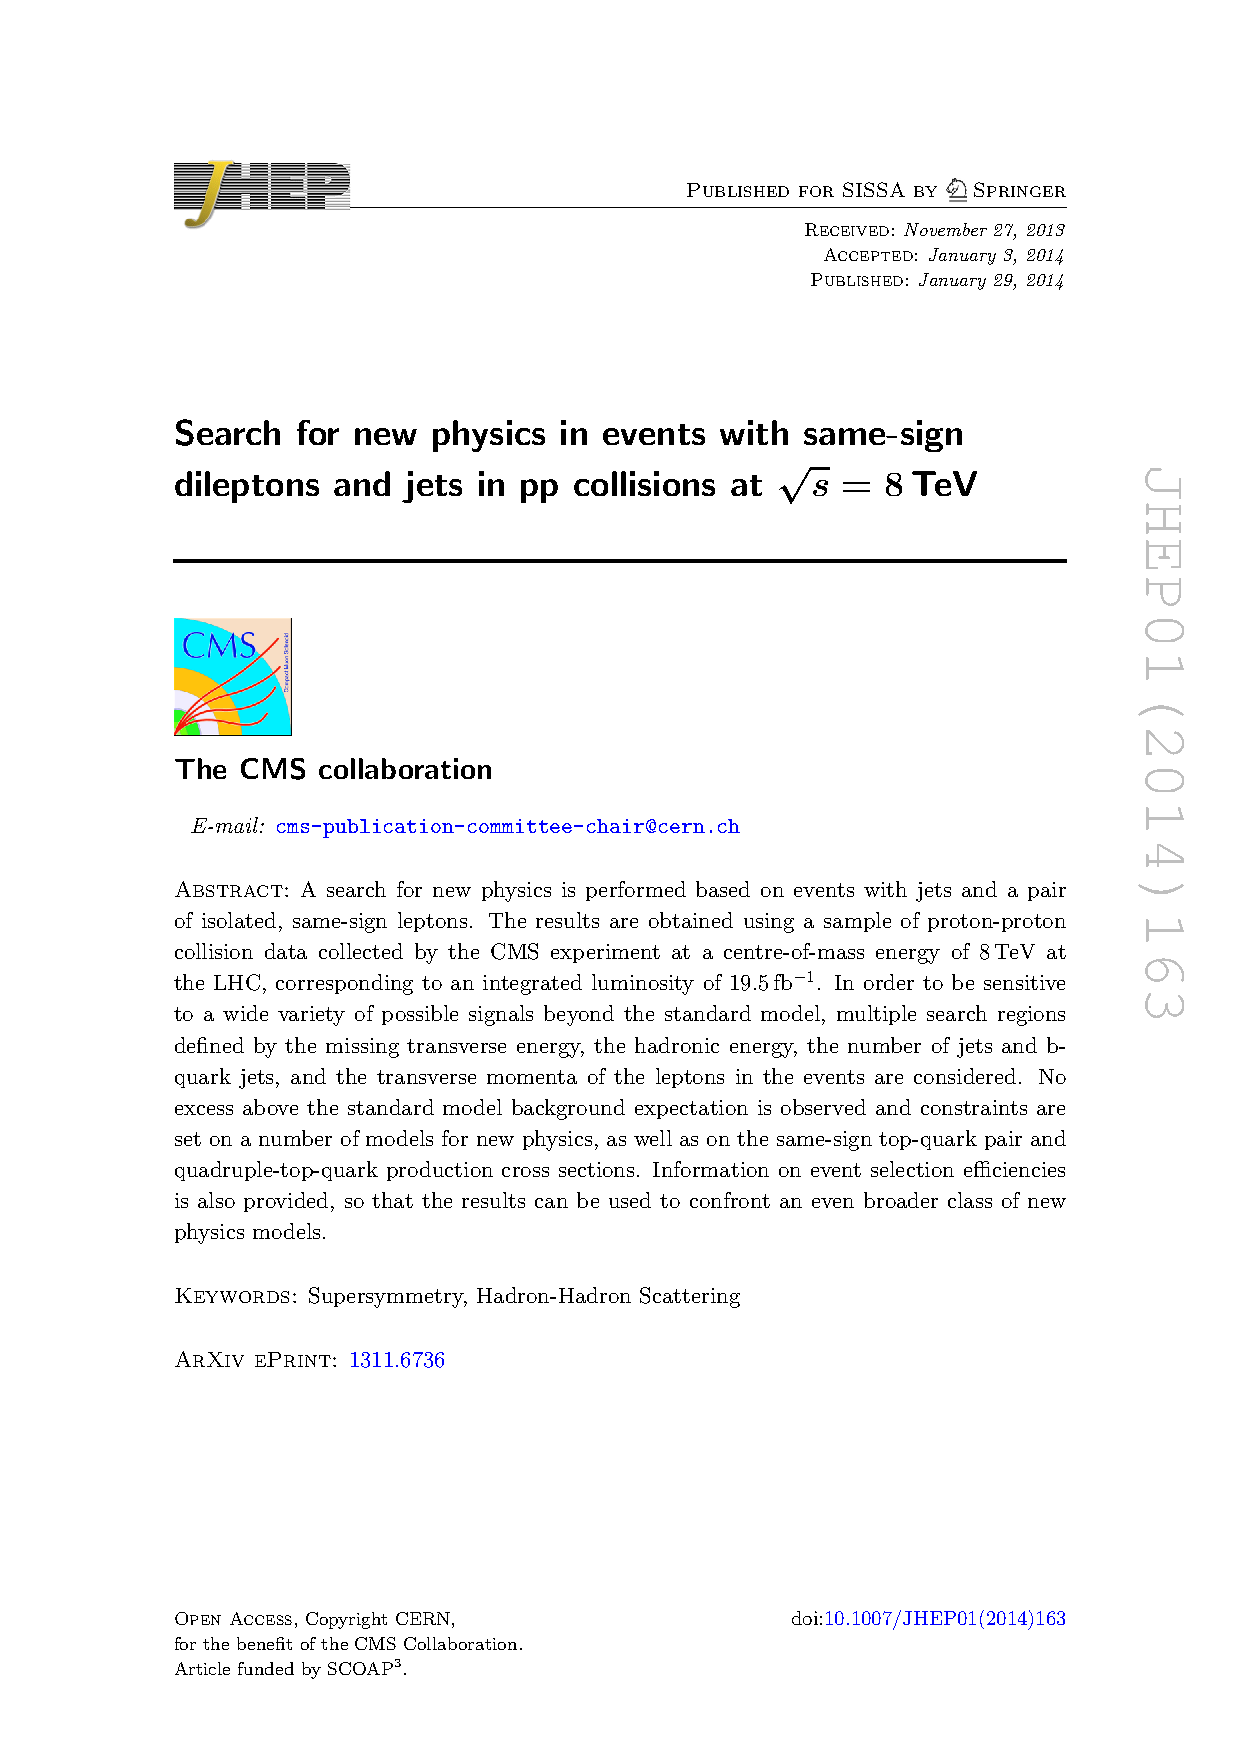
\includepdf[pages={1,2,3}]{Articulos/ArticulosReducidos/Investigacion_Publicaciones_Search_for_new_physics_in_events_with_same-sign_dileptons_and_jet.pdf}
\subsubsection{Searches for Supersymmetry using the MT2 Variable in Hadronic Events Produced in pp Collisions at 8 TeV}
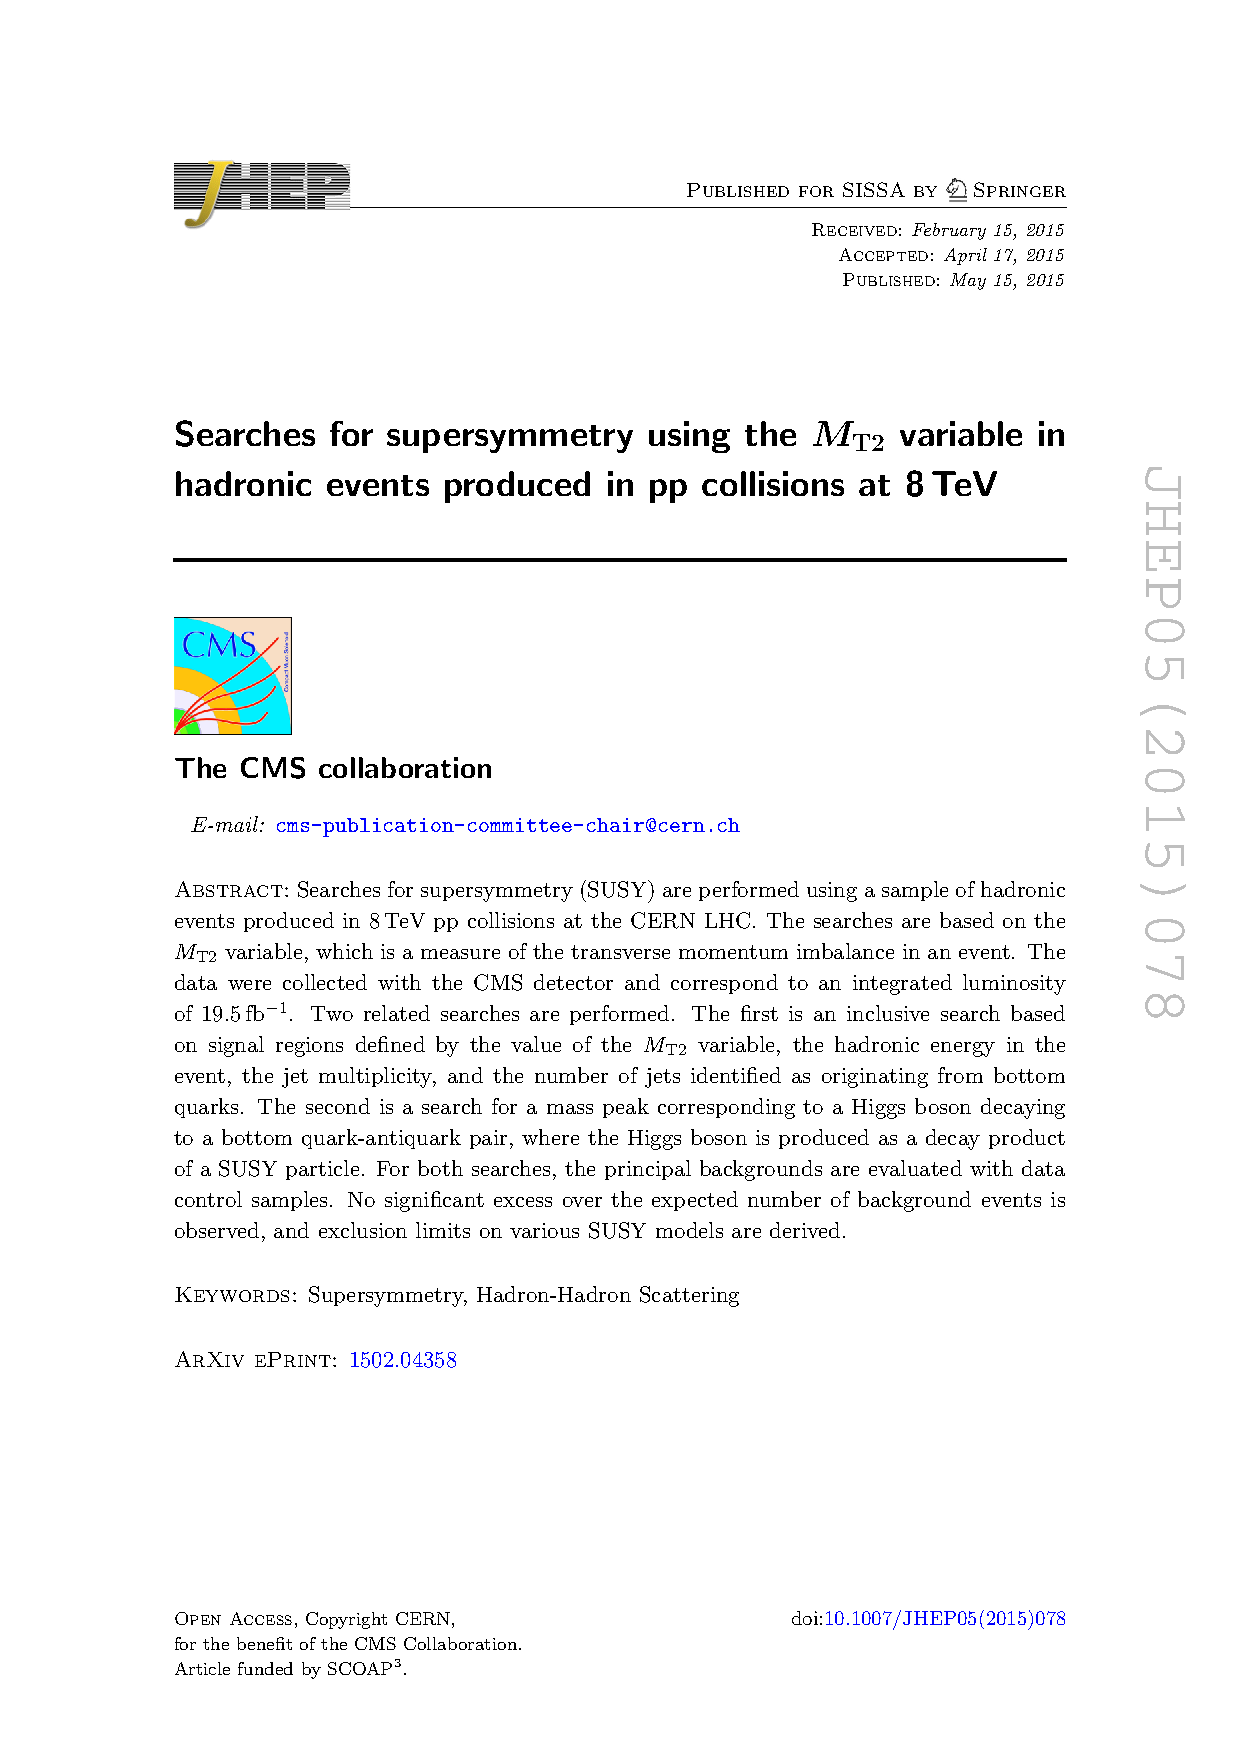
\includepdf[pages={1,2,3}]{Articulos/ArticulosReducidos/Investigacion_Publicaciones_Searches_for_Supersymmetry_using_the_MT2_Variable_in_Hadronic_Eve.pdf}
\subsubsection{Search for Physics Beyond the Standard Model in Events with Two Leptons Jets and Missing Transverse Momentum in pp Collisions at sqrt s 8 TeV}
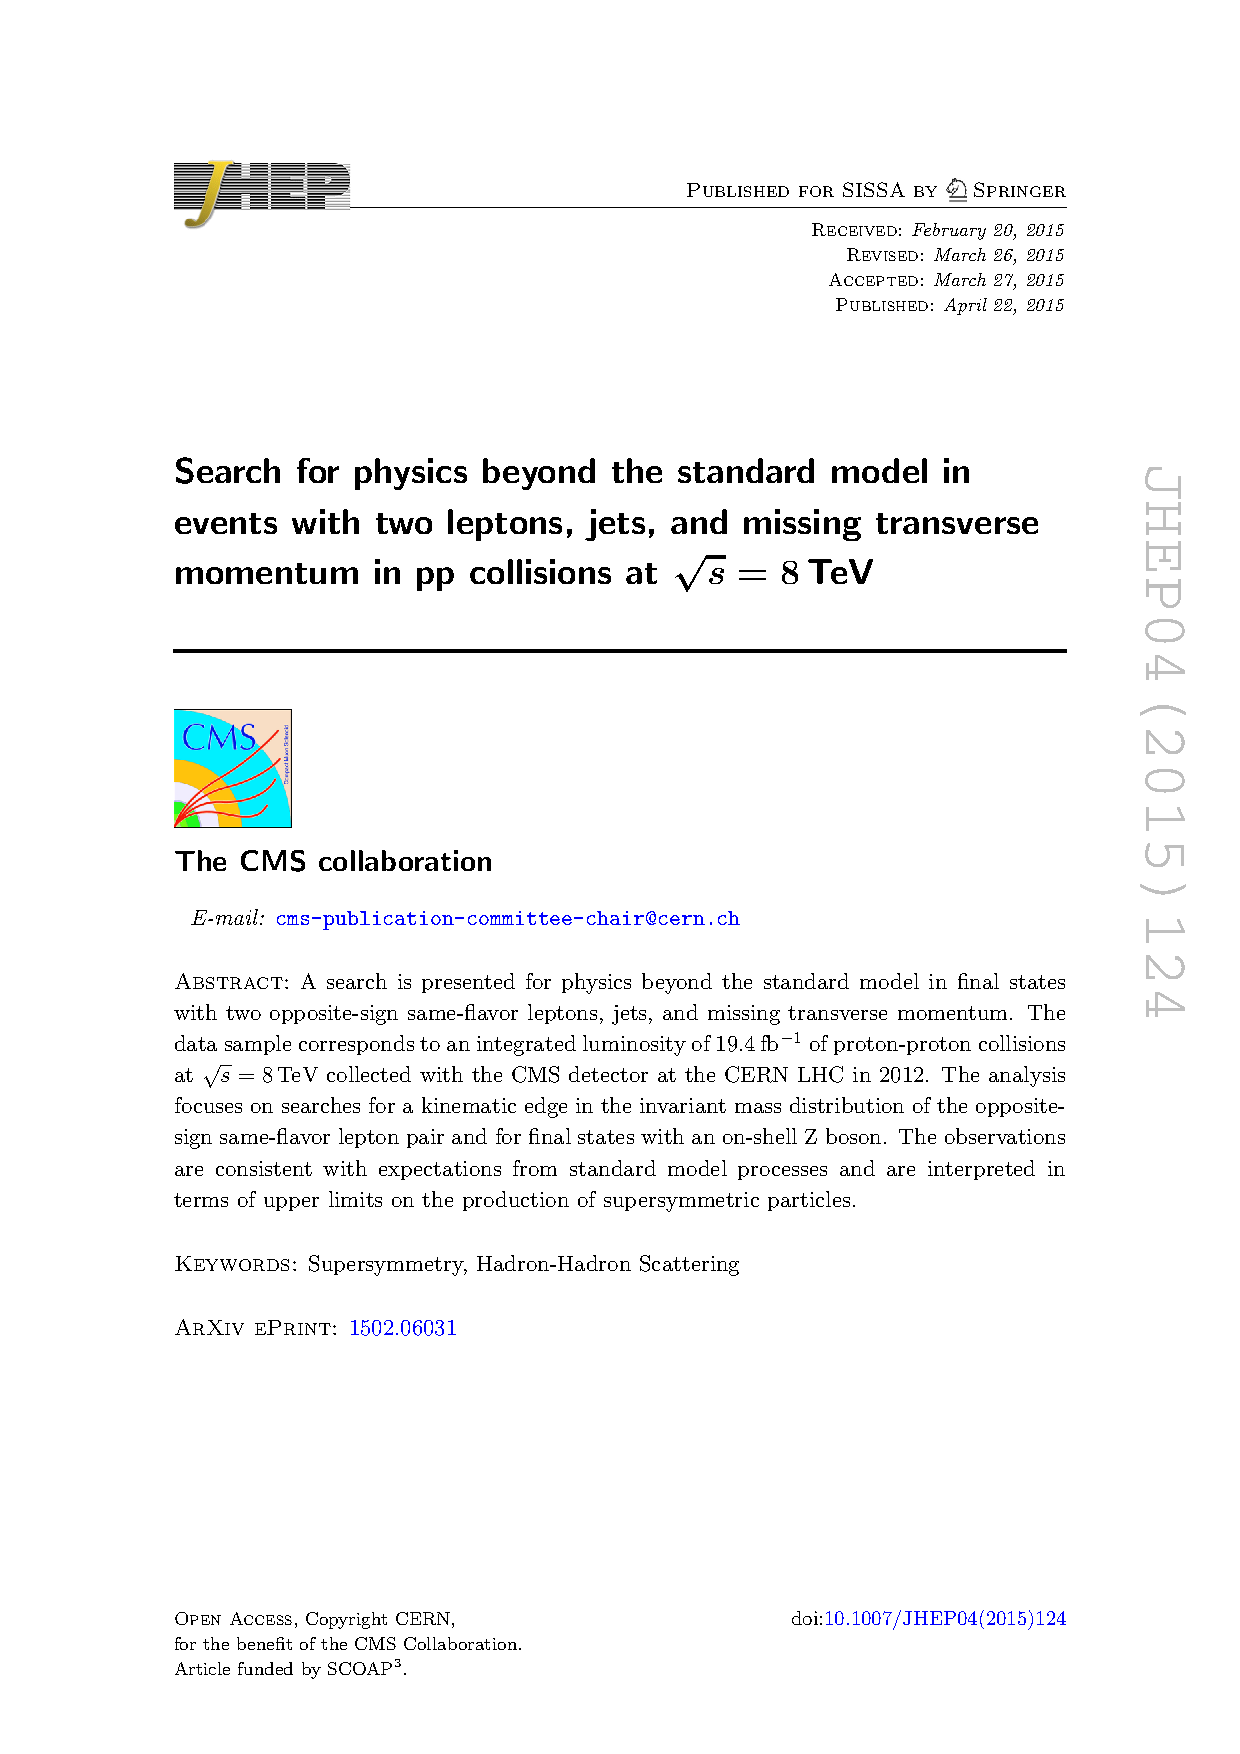
\includepdf[pages={1,2,3}]{Articulos/ArticulosReducidos/Investigacion_Publicaciones_Search_for_Physics_Beyond_the_Standard_Model_in_Events_with_Two_L.pdf}
\subsubsection{Search for supersymmetry in the multijet and missing transverse momentum final state in pp collisions at 13 TeV}
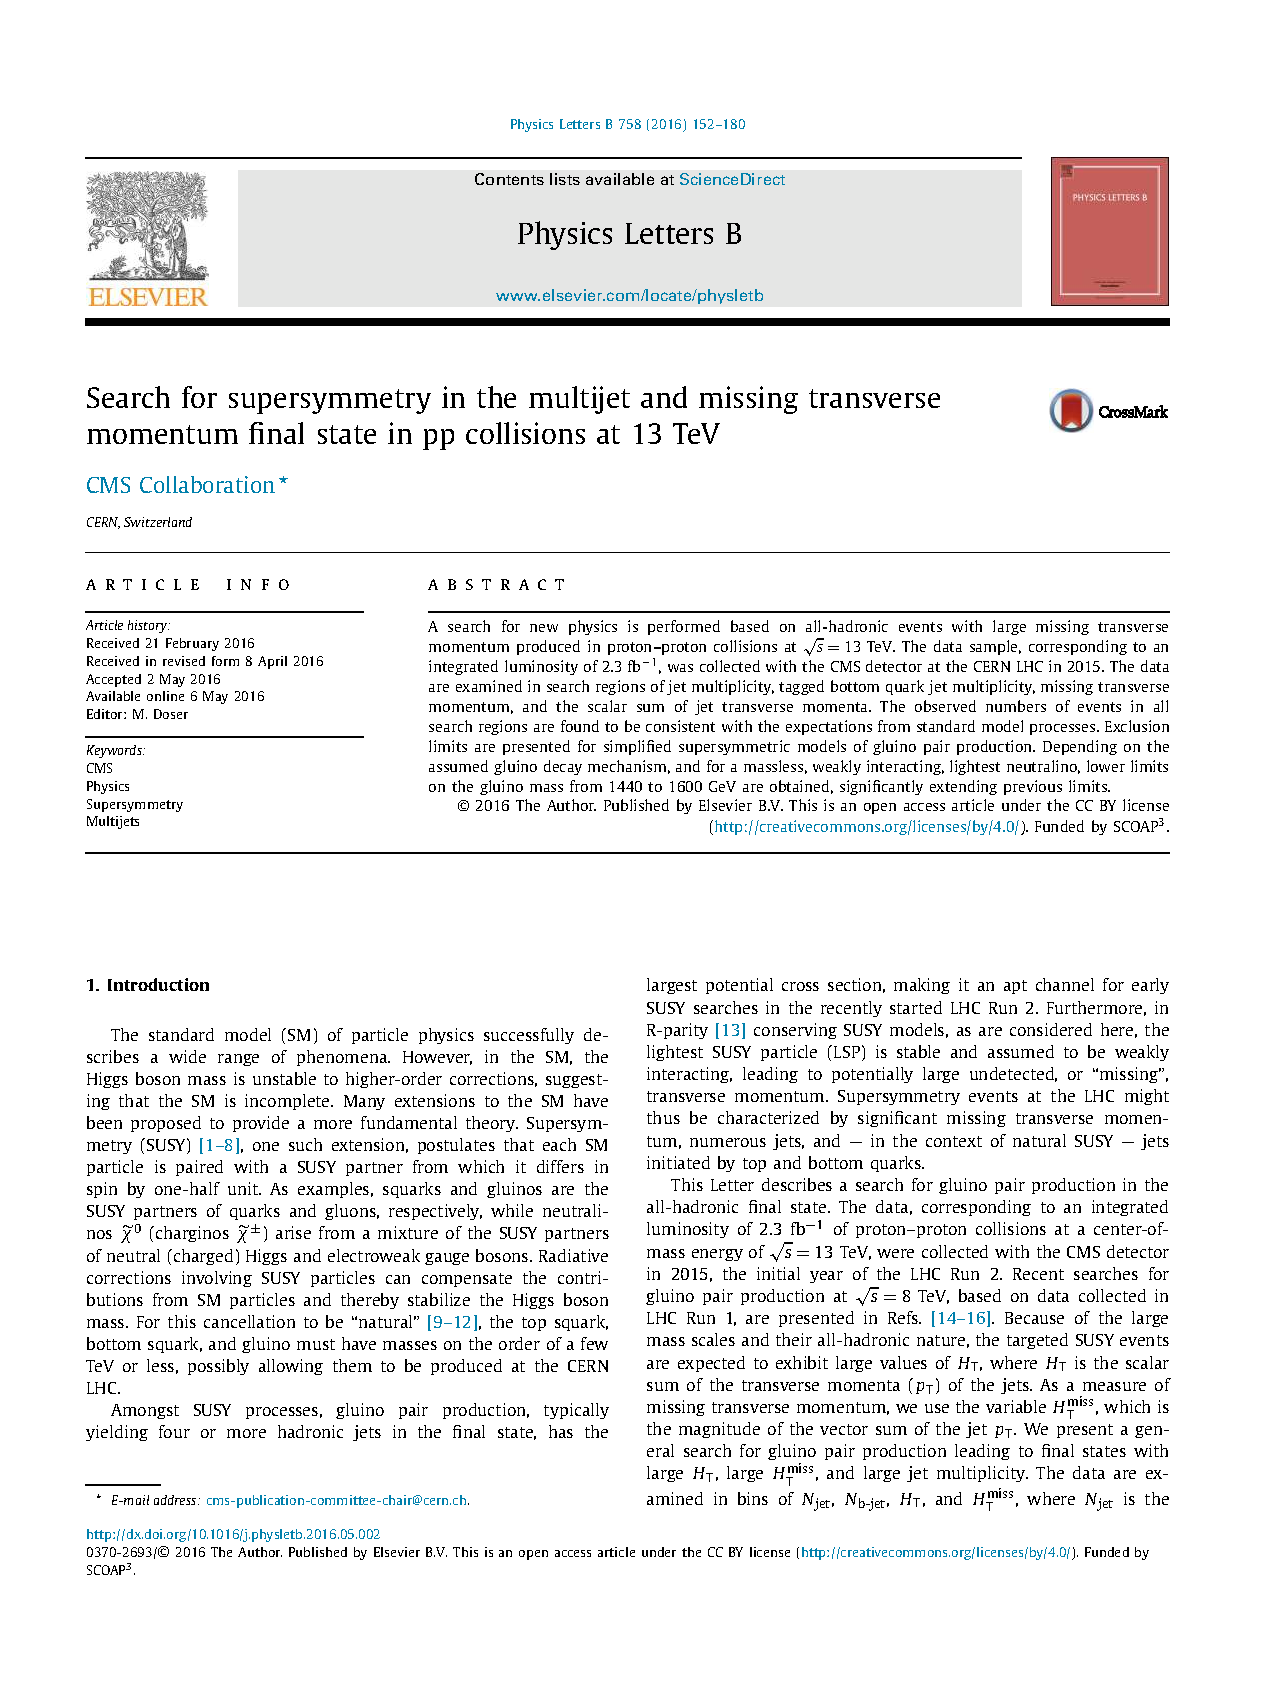
\includepdf[pages={1,2,3}]{Articulos/ArticulosReducidos/Investigacion_Publicaciones_Search_for_supersymmetry_in_the_multijet_and_missing_transverse_m.pdf}
\subsubsection{Search for new physics with the MT2 variable in all-jets final states produced in pp collisions at sqrt s 13 TeV}
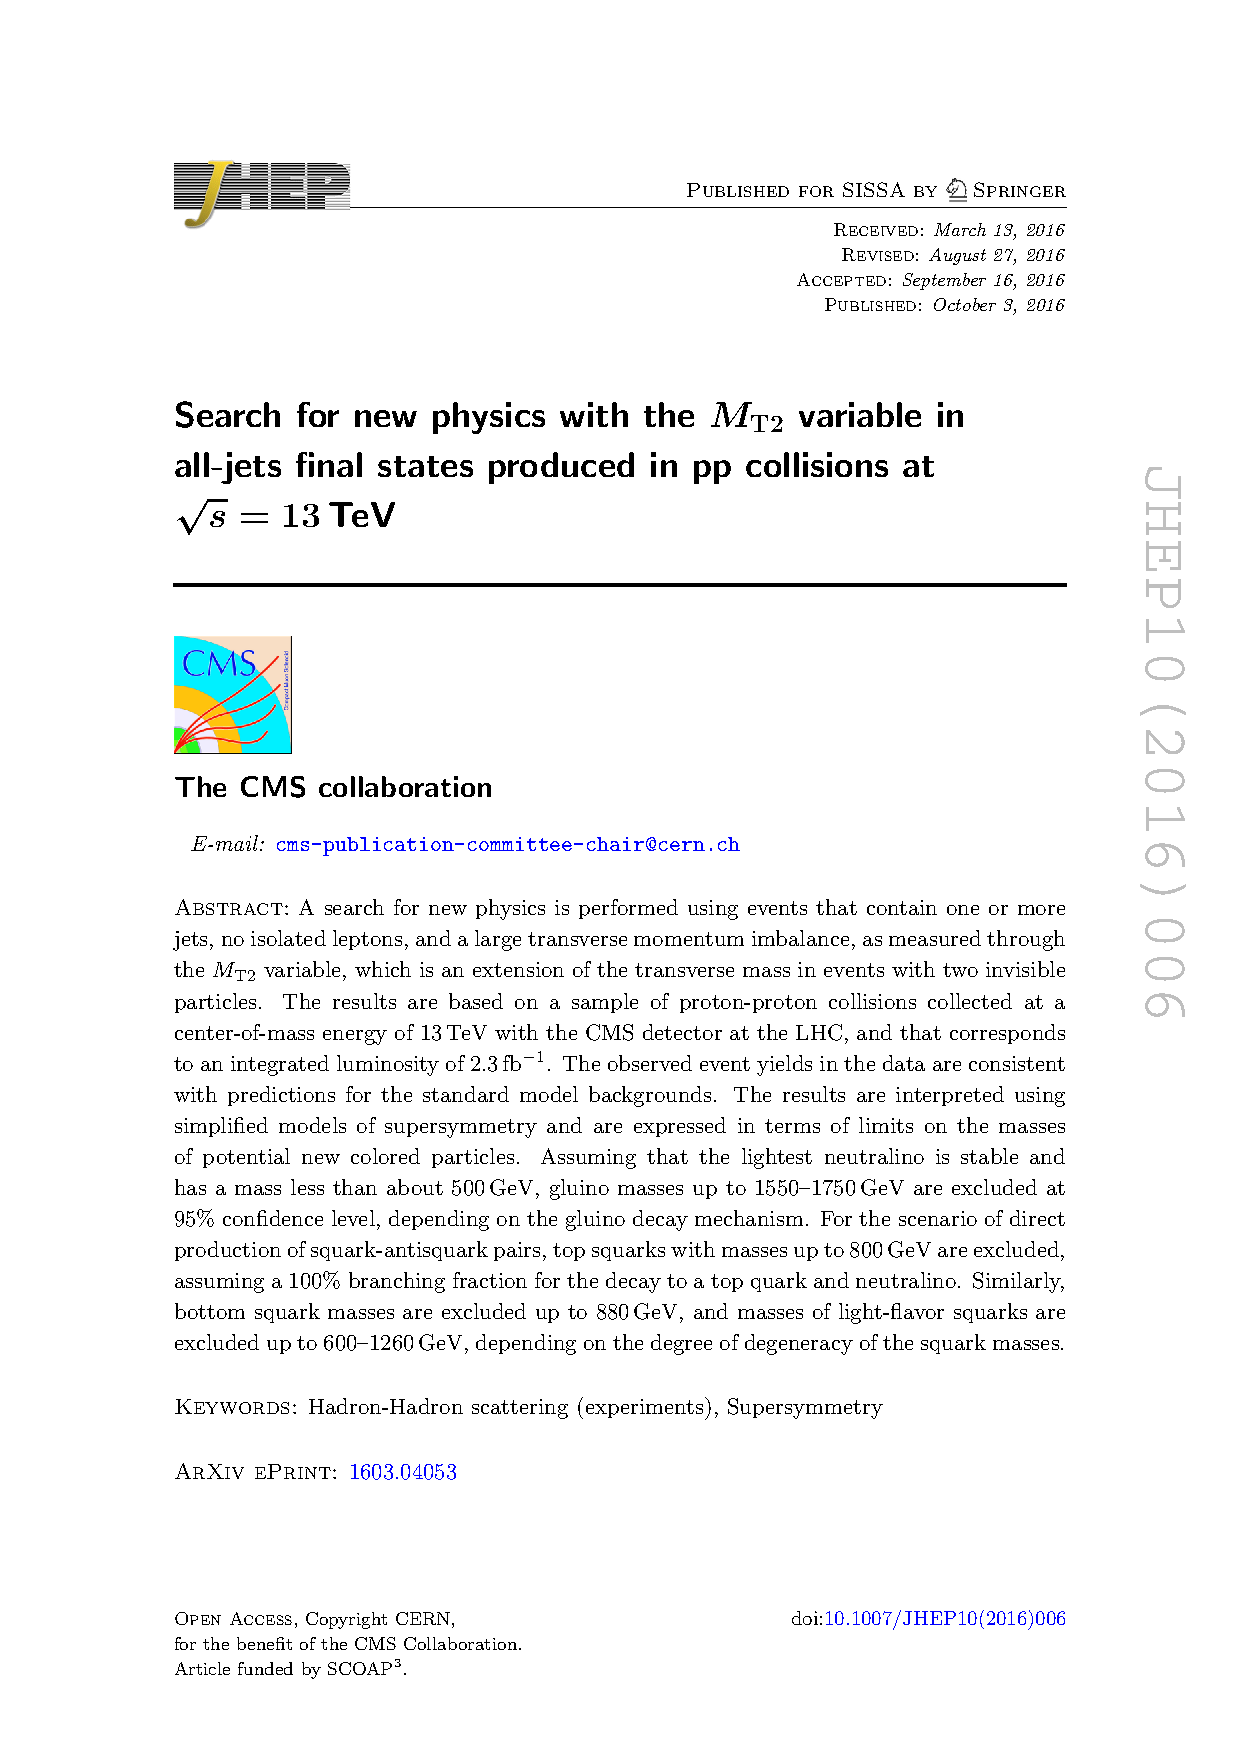
\includepdf[pages={1,2,3}]{Articulos/ArticulosReducidos/Investigacion_Publicaciones_Search_for_new_physics_with_the_MT2_variable_in_all-jets_final_st.pdf}
\subsubsection{Inclusive search for supersymmetry using razor variables in pp collisions at  sqrt s 13 TeV}
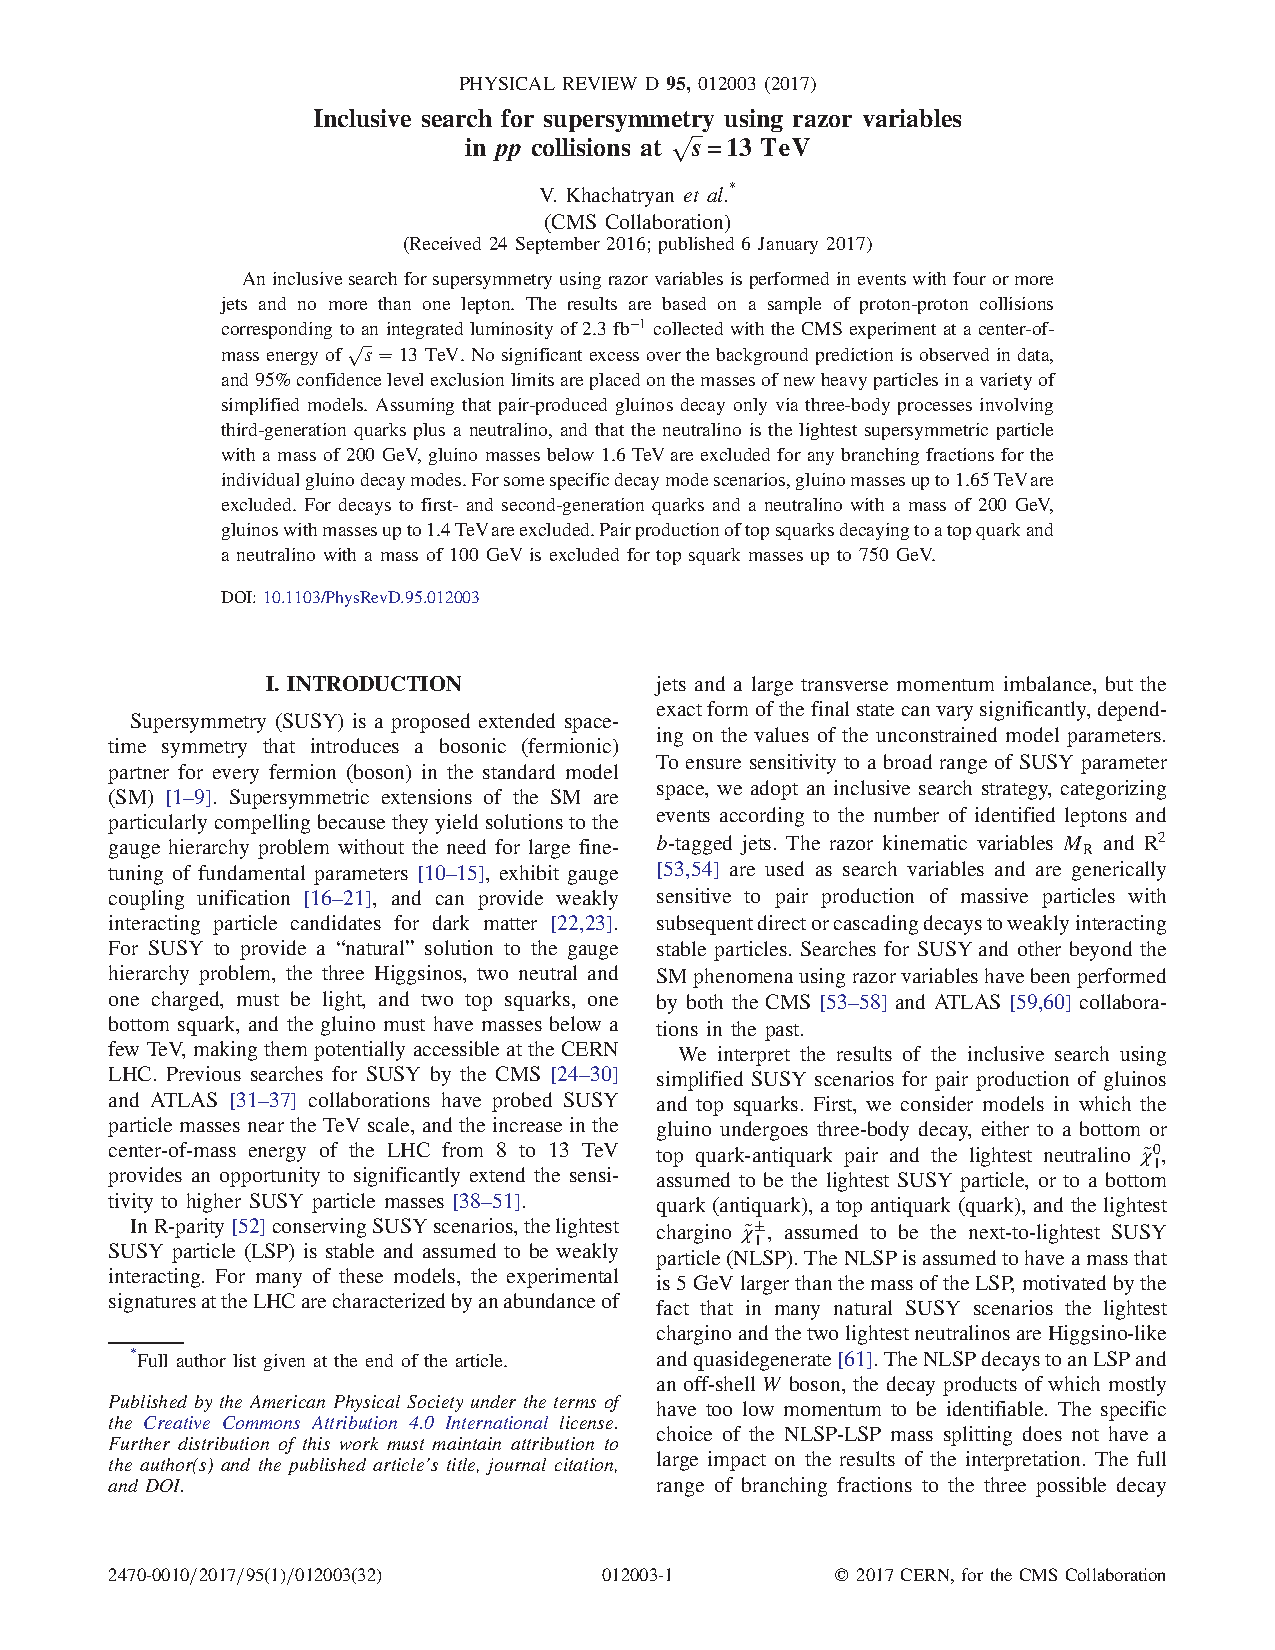
\includepdf[pages={1,2,3}]{Articulos/ArticulosReducidos/Investigacion_Publicaciones_Inclusive_search_for_supersymmetry_using_razor_variables_in_pp_co.pdf}
\subsubsection{Search for supersymmetry in pp collisions at sqrt s 13 TeV in the single-lepton final state using the sum of masses of large-radius jets}
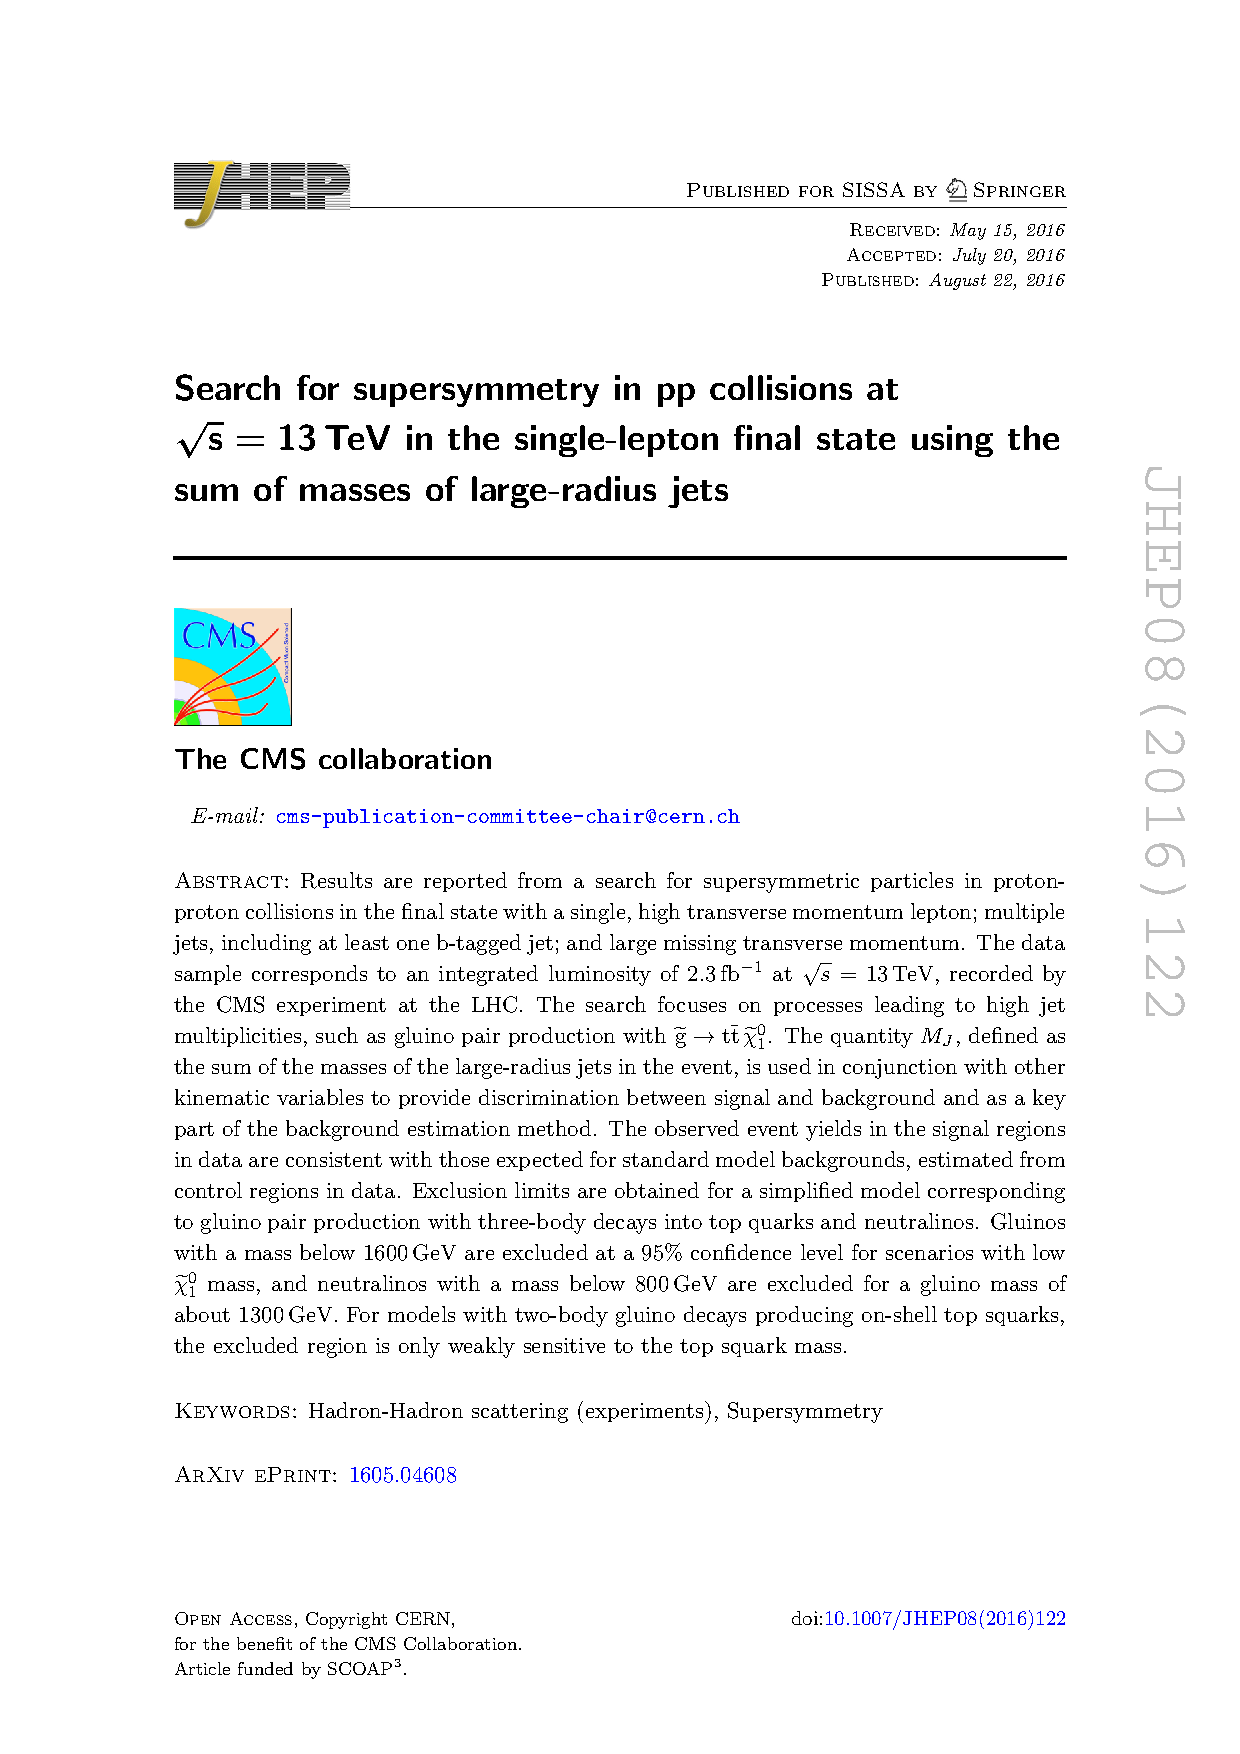
\includepdf[pages={1,2,3}]{Articulos/ArticulosReducidos/Investigacion_Publicaciones_Search_for_supersymmetry_in_pp_collisions_at_sqrt_s_13_TeV_in_the.pdf}
\subsubsection{Search for new physics in same-sign dilepton events in proton–proton collisions at sqrt s 13 TeV}
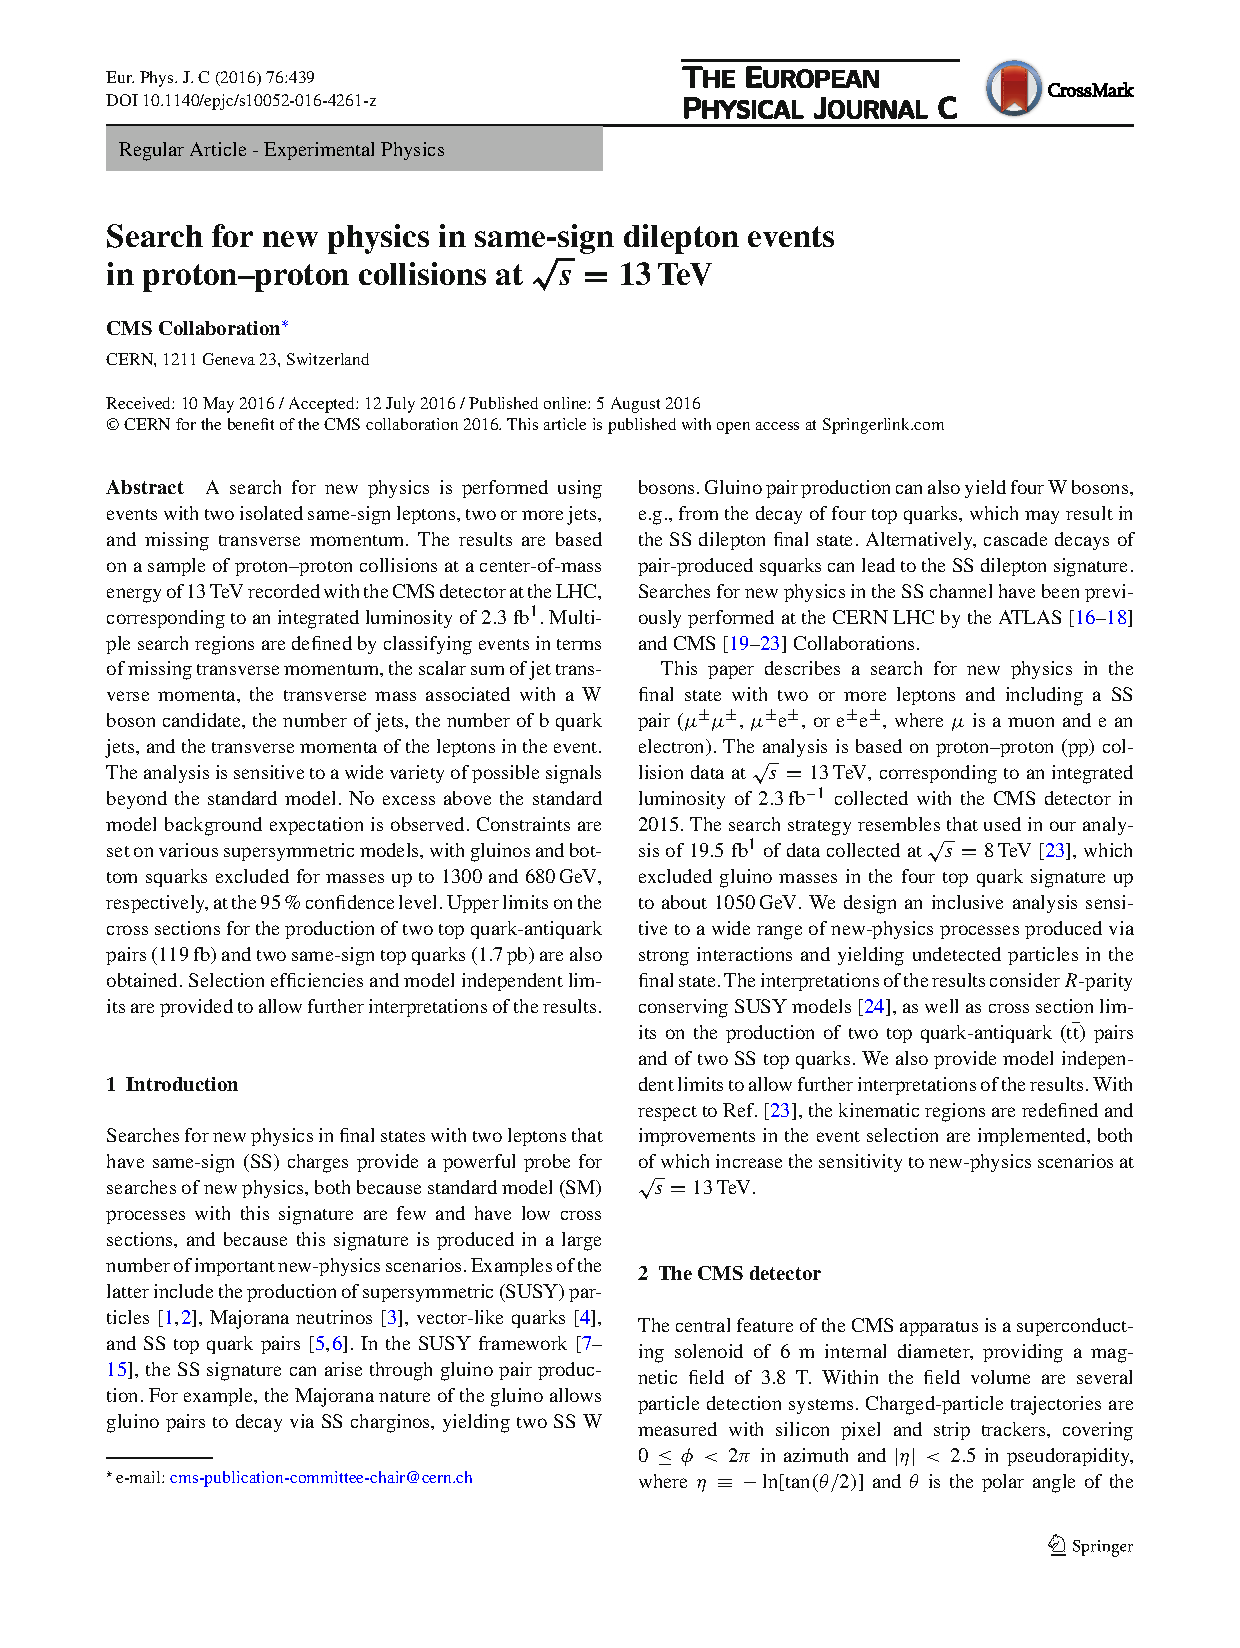
\includepdf[pages={1,2,3}]{Articulos/ArticulosReducidos/Investigacion_Publicaciones_Search_for_new_physics_in_same-sign_dilepton_events_in_proton_p.pdf}
\subsubsection{Phenomenological MSSM interpretation of CMS searches in pp collisions at sqrt s 7 and 8 TeV}
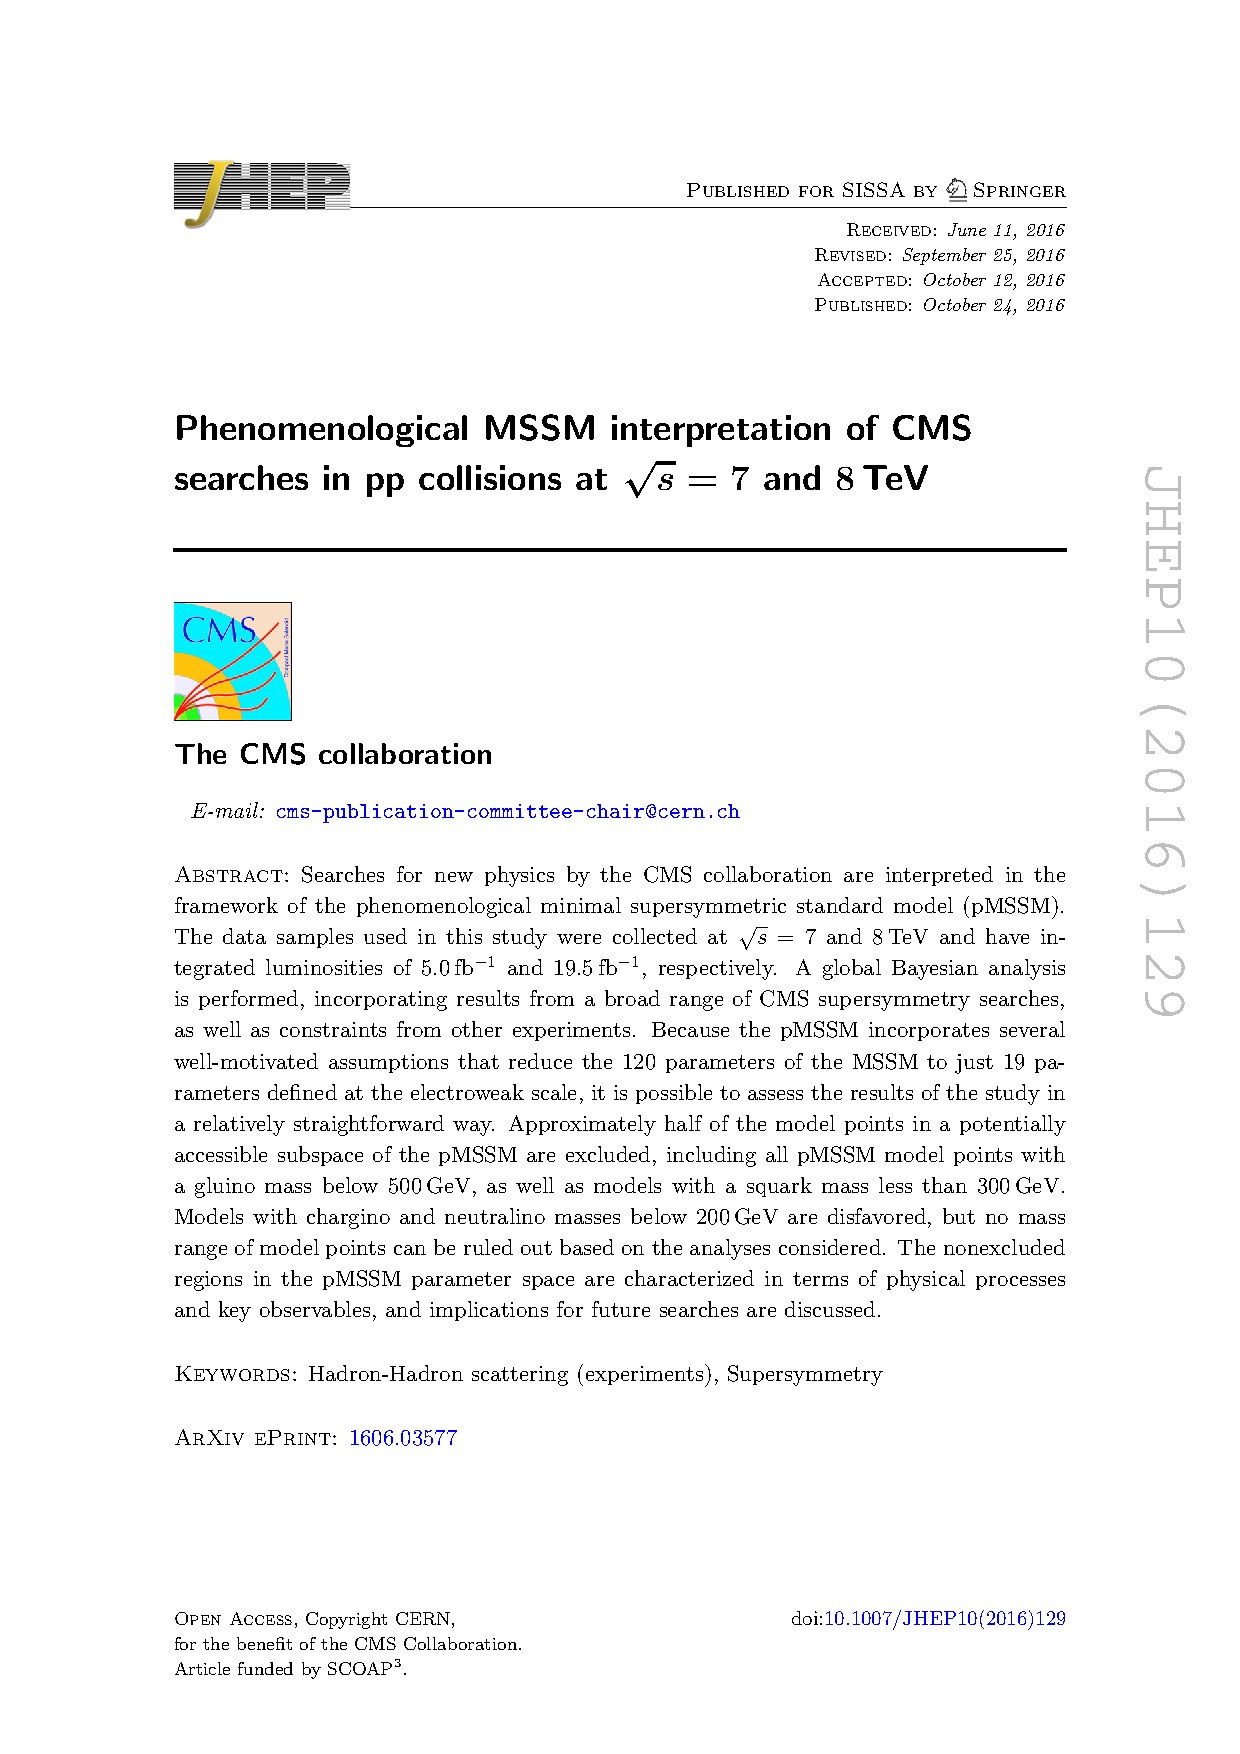
\includepdf[pages={1,2,3}]{Articulos/ArticulosReducidos/Investigacion_Publicaciones_Phenomenological_MSSM_interpretation_of_CMS_searches_in_pp_collis.pdf}
\subsubsection{Search for new physics in final states with two opposite-sign same-flavor leptons jets and missing transverse momentum in pp collisions at sqrt s 13 TeV}
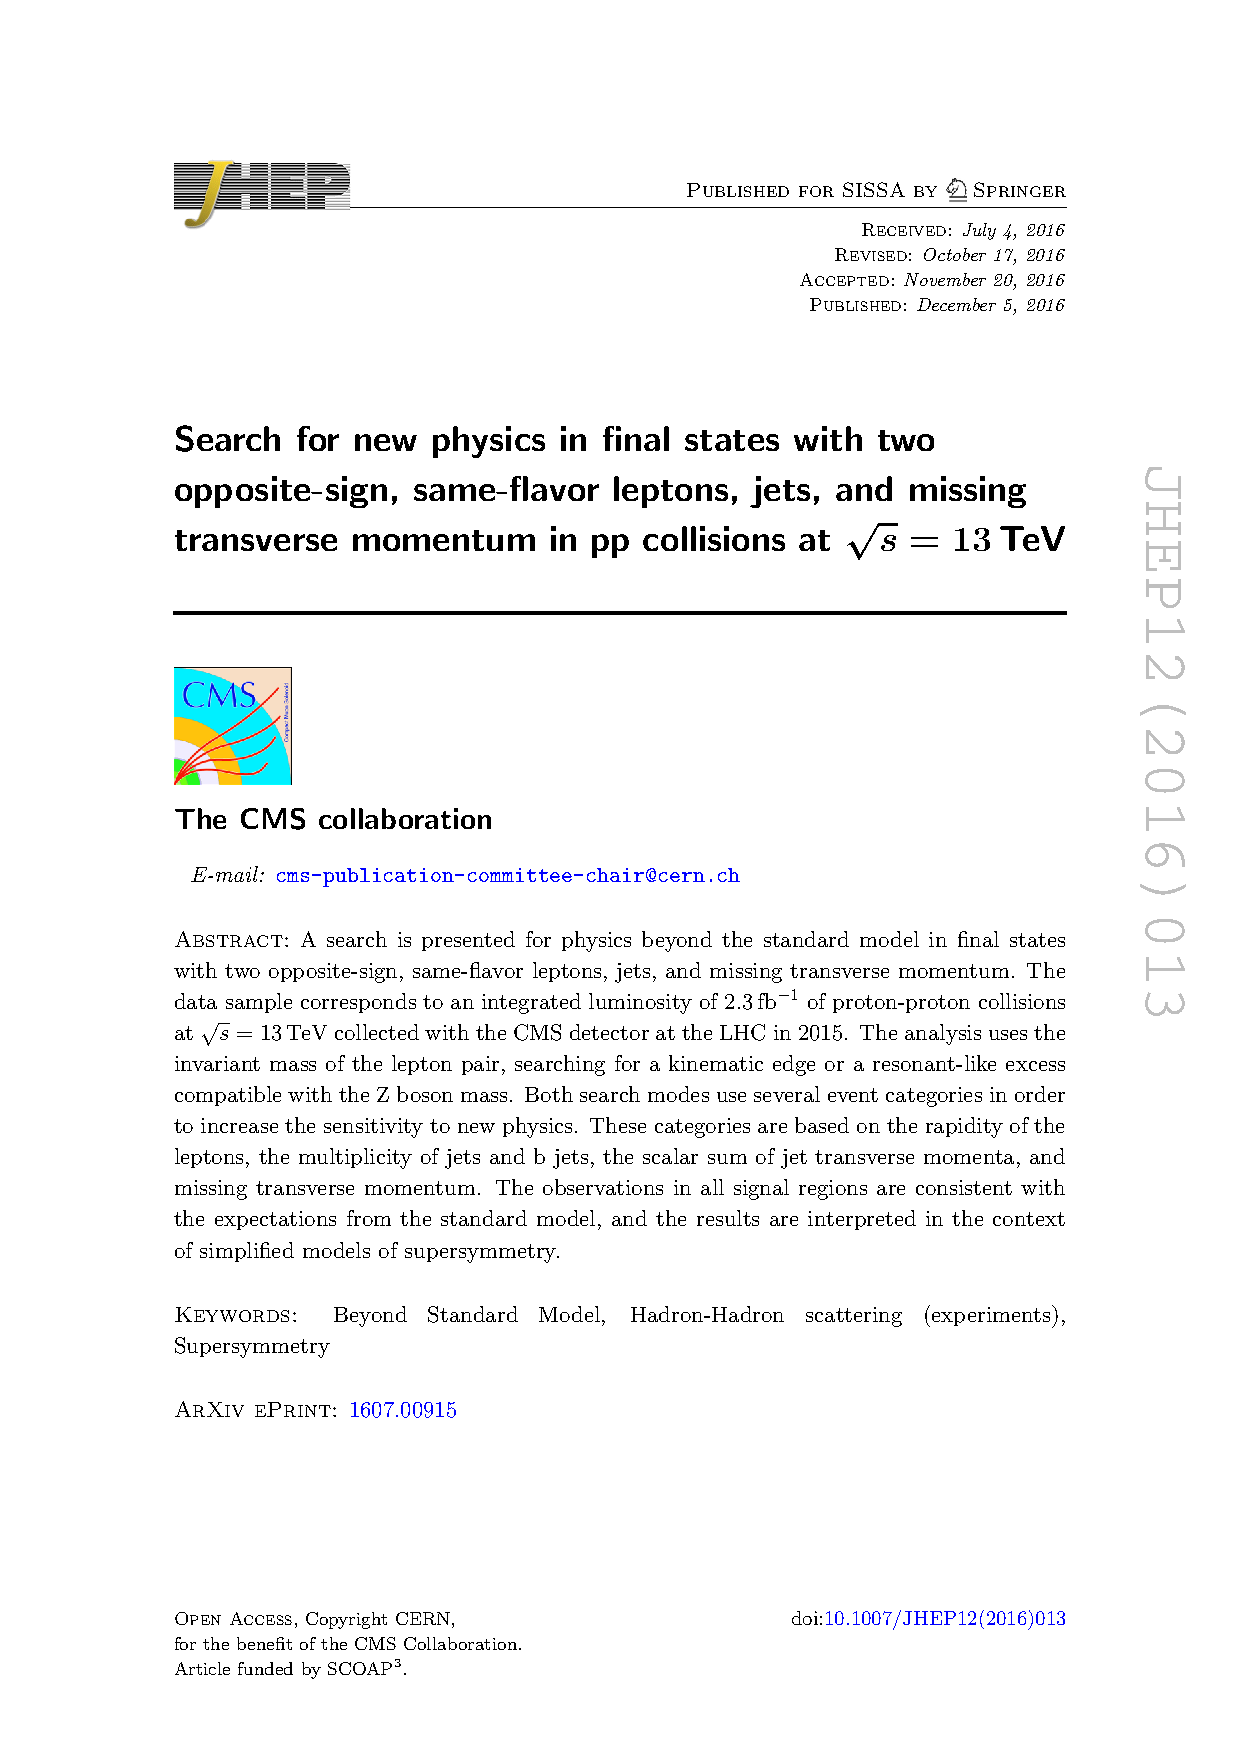
\includepdf[pages={1,2,3}]{Articulos/ArticulosReducidos/Investigacion_Publicaciones_Search_for_new_physics_in_final_states_with_two_opposite-sign_sam.pdf}
\subsubsection{Search for physics beyond the standard model in events with two leptons of same sign missing transverse momentum and jets in proton-proton collisions at sqrt s 13 TeV}
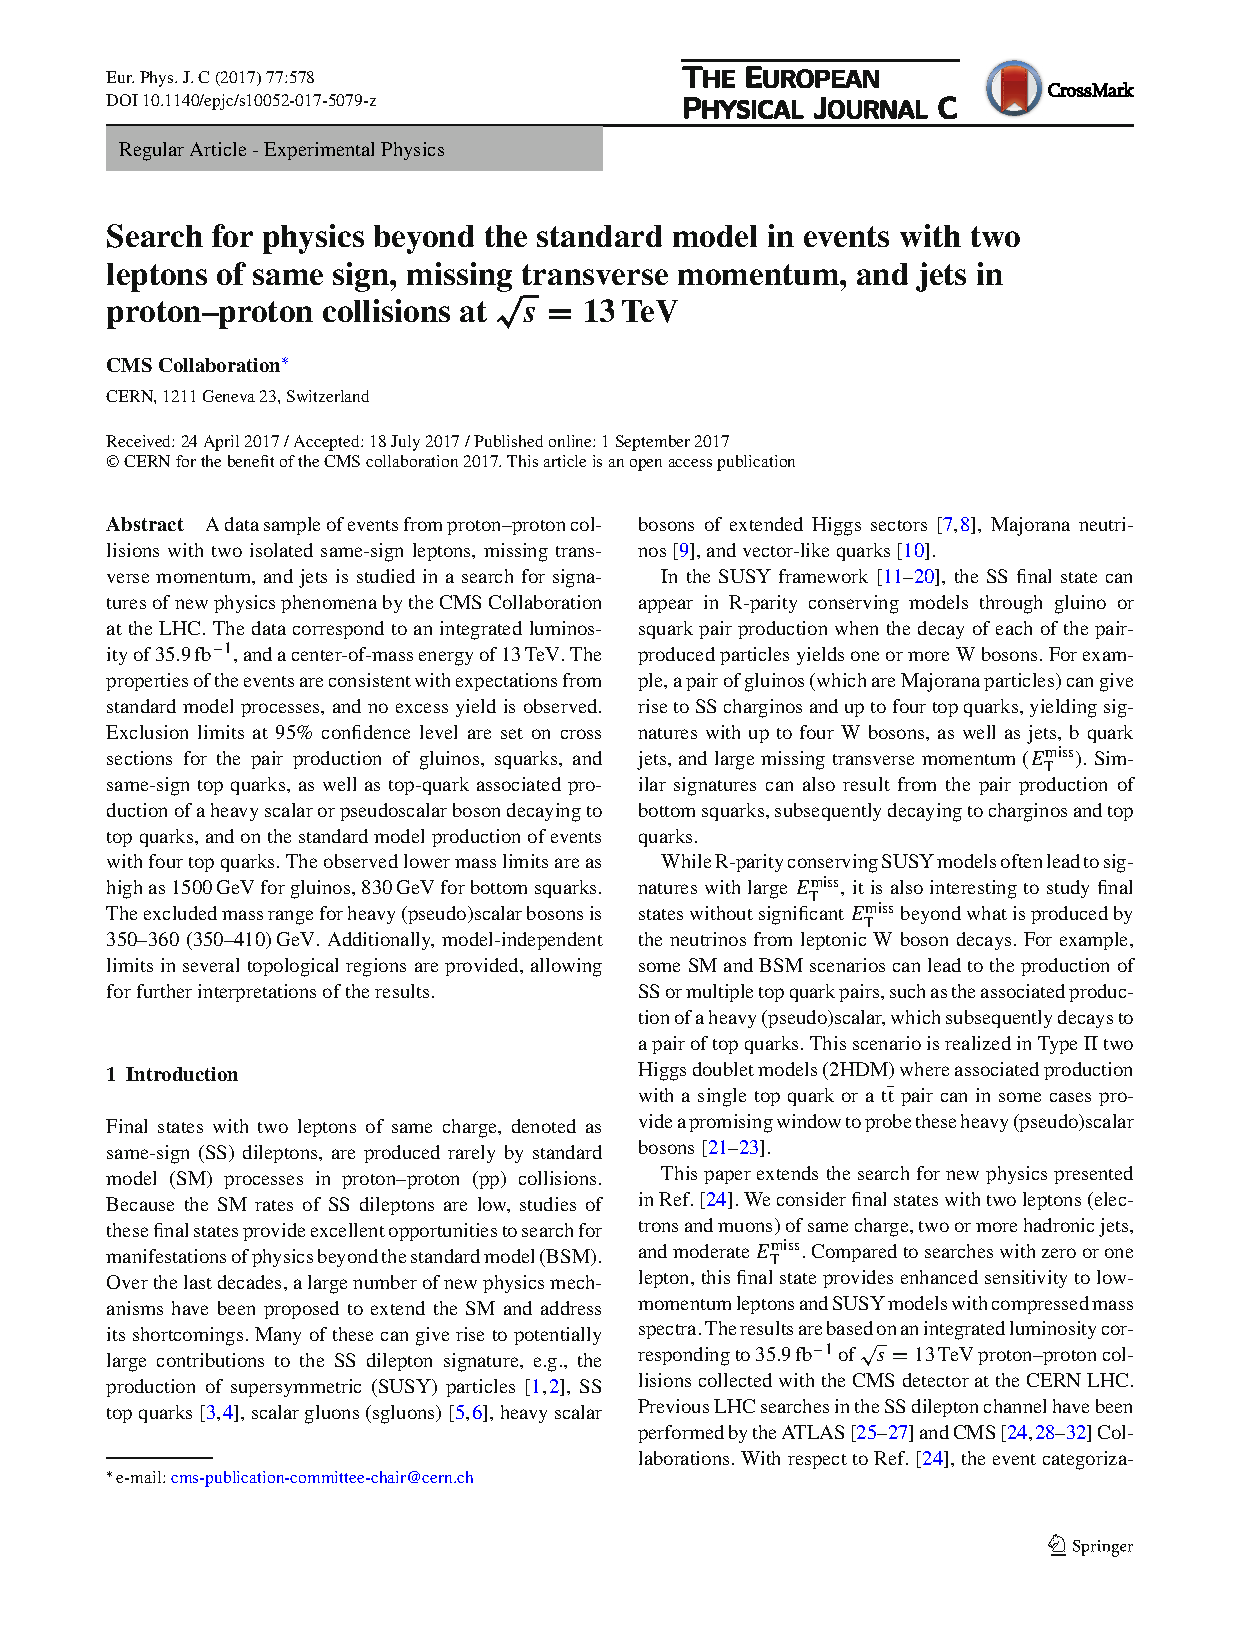
\includepdf[pages={1,2,3}]{Articulos/ArticulosReducidos/Investigacion_Publicaciones_Search_for_physics_beyond_the_standard_model_in_events_with_two_l.pdf}
\subsubsection{Search for direct production of supersymmetric partners of the top quark in the all-jets final state in proton-proton collisions at sqrt s 13 TeV}
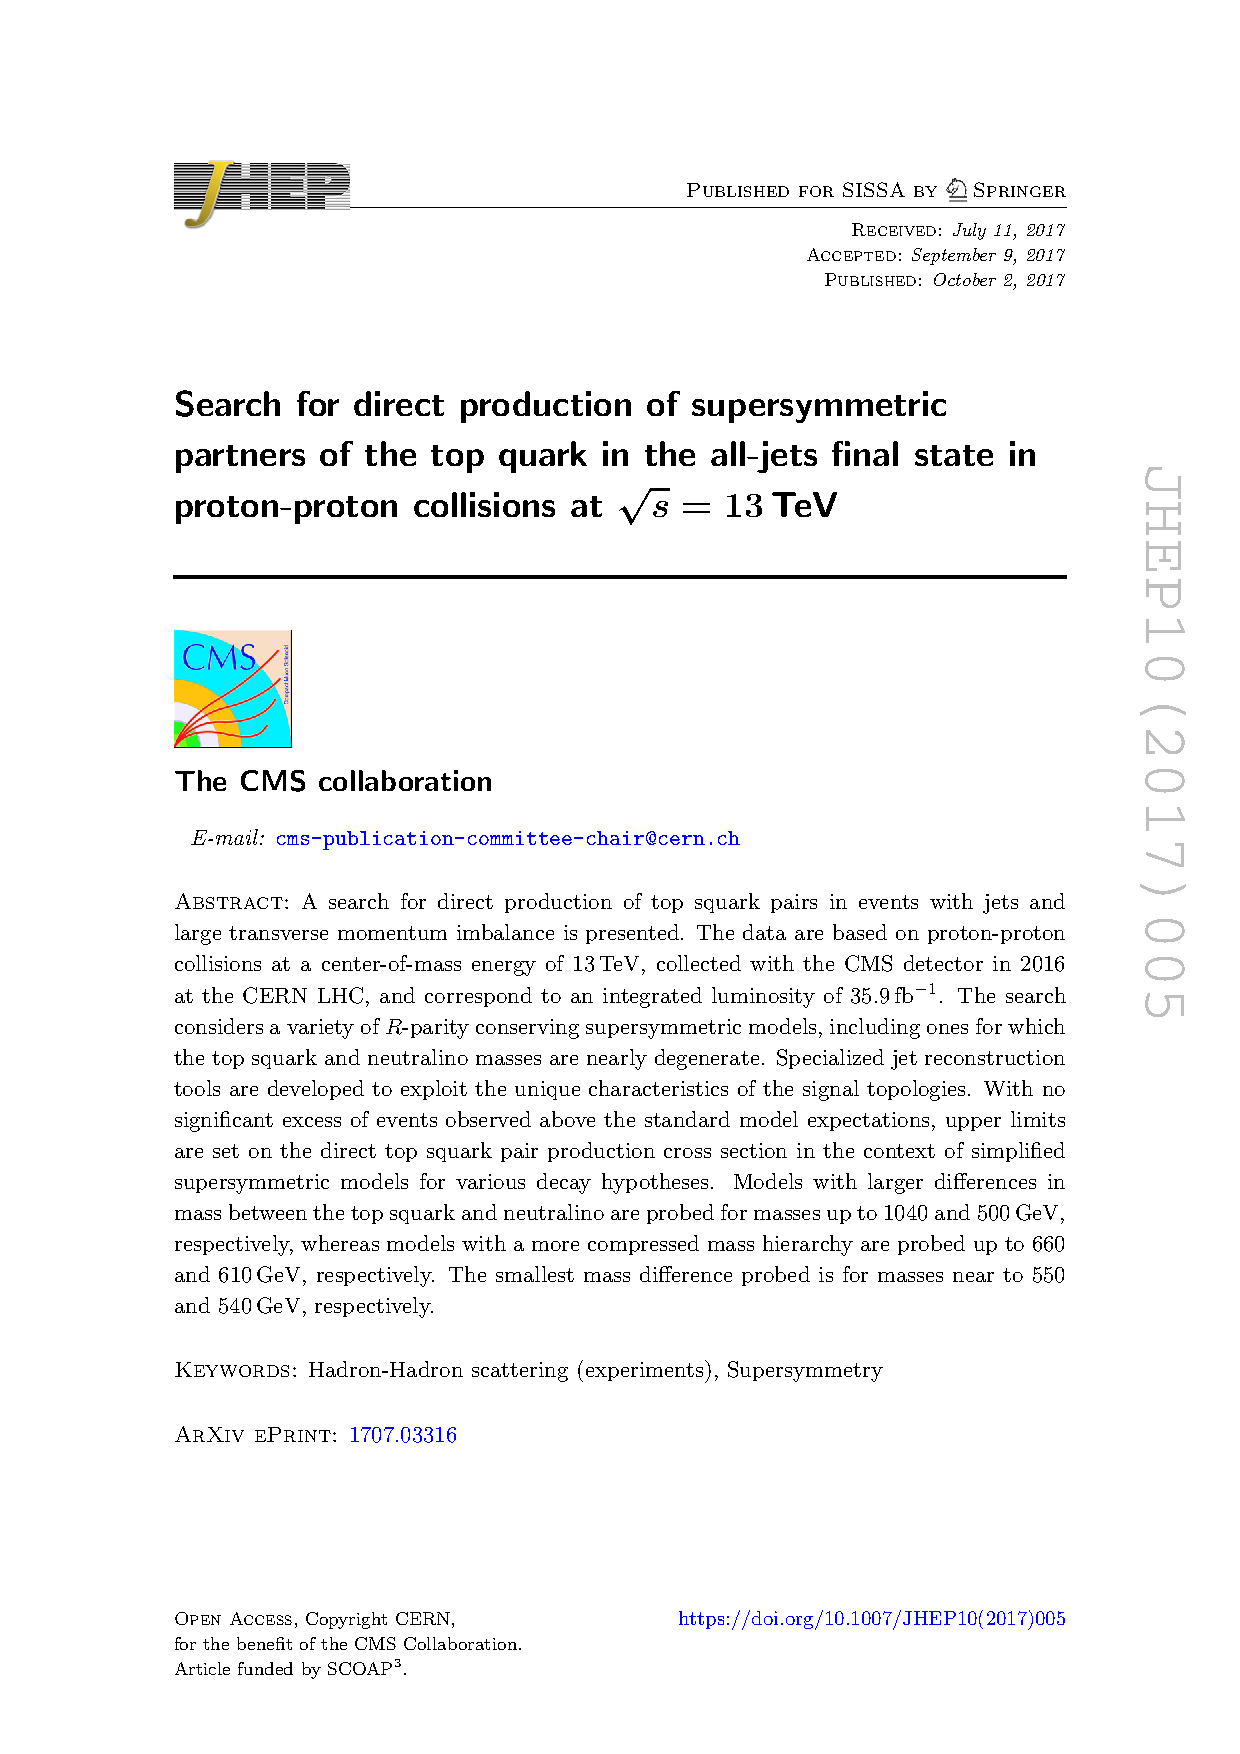
\includepdf[pages={1,2,3}]{Articulos/ArticulosReducidos/Investigacion_Publicaciones_Search_for_direct_production_of_supersymmetric_partners_of_the_to.pdf}
\subsubsection{Search for top squark pair production in pp collisions at sqrt s 13 TeV using single lepton events}
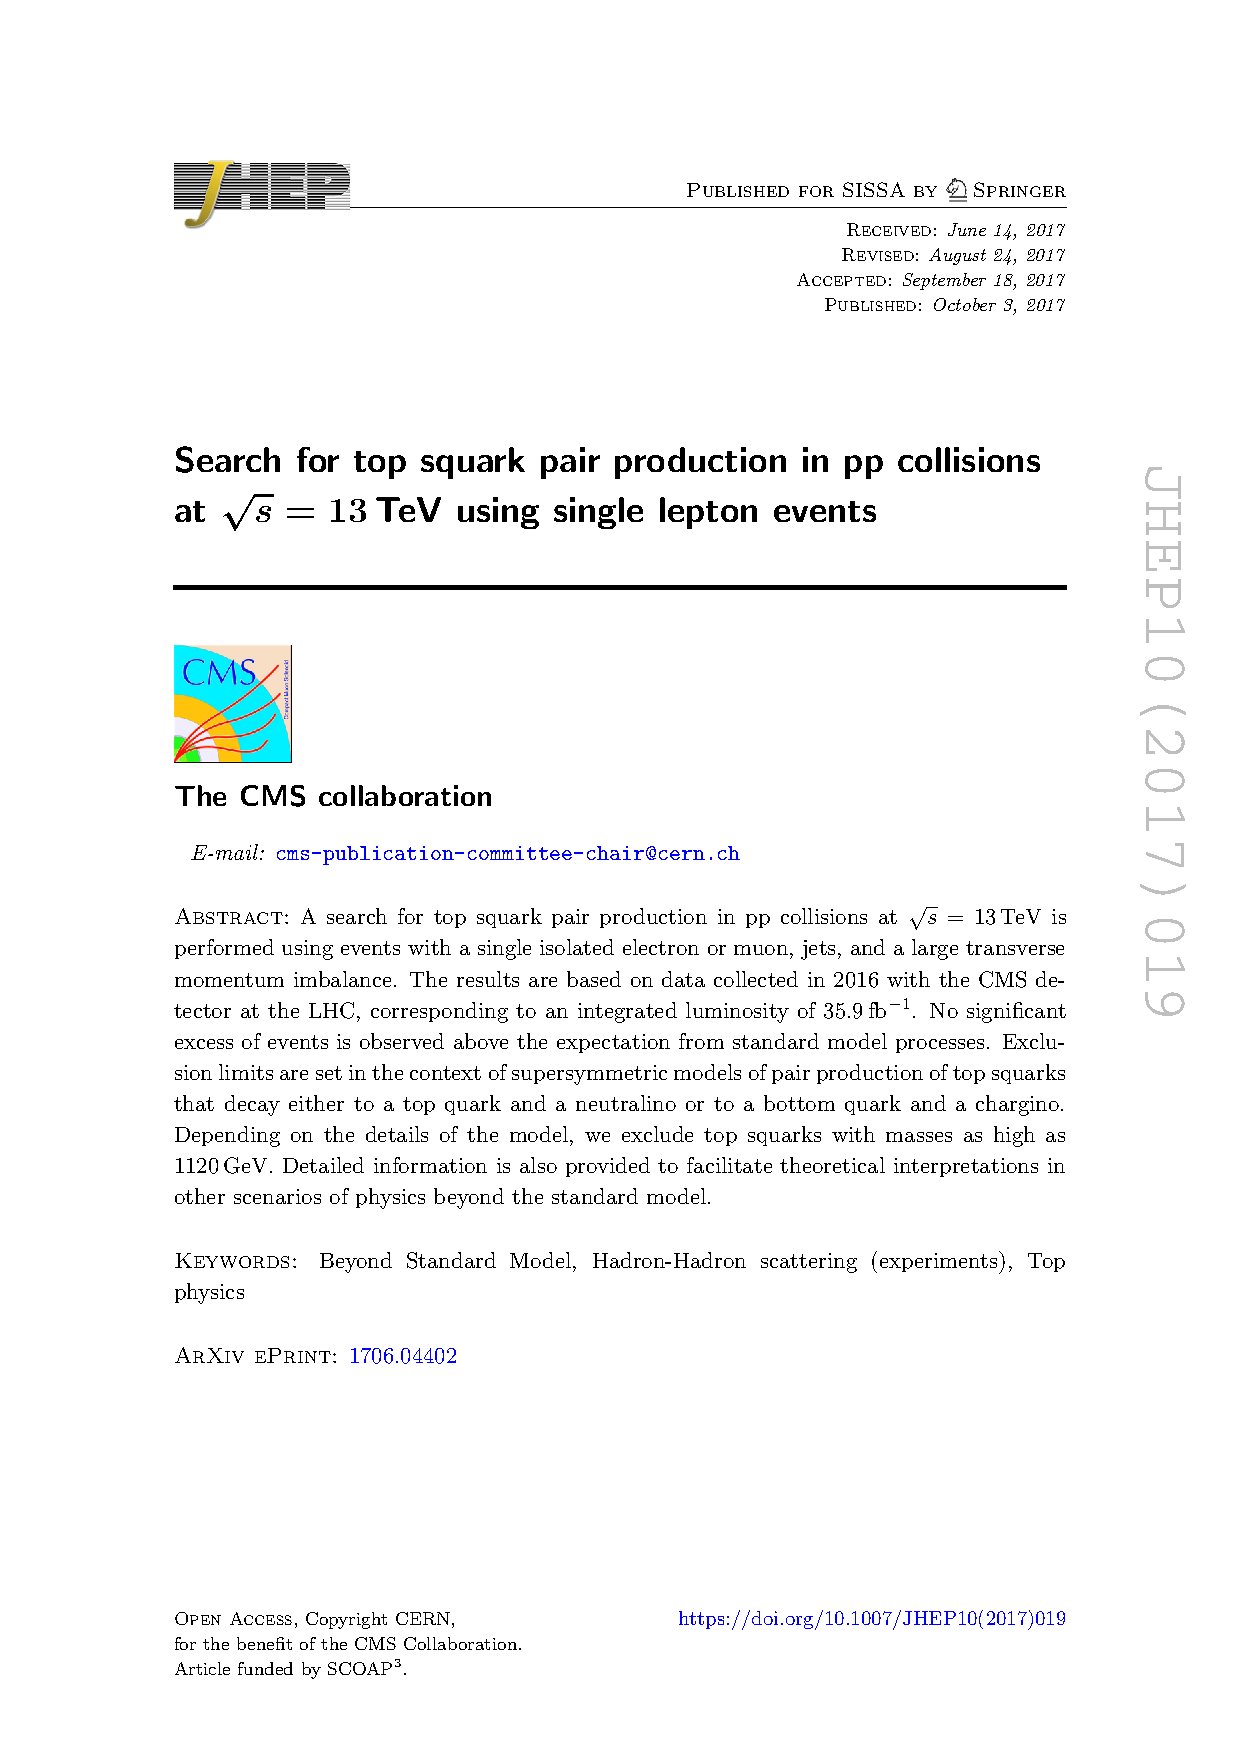
\includepdf[pages={1,2,3}]{Articulos/ArticulosReducidos/Investigacion_Publicaciones_Search_for_top_squark_pair_production_in_pp_collisions_at_sqrt_s_.pdf}
\subsubsection{Search for new phenomena with the MT2 variable in the all-hadronic final state produced in proton-proton collisions at sqrt s 13 TeV}
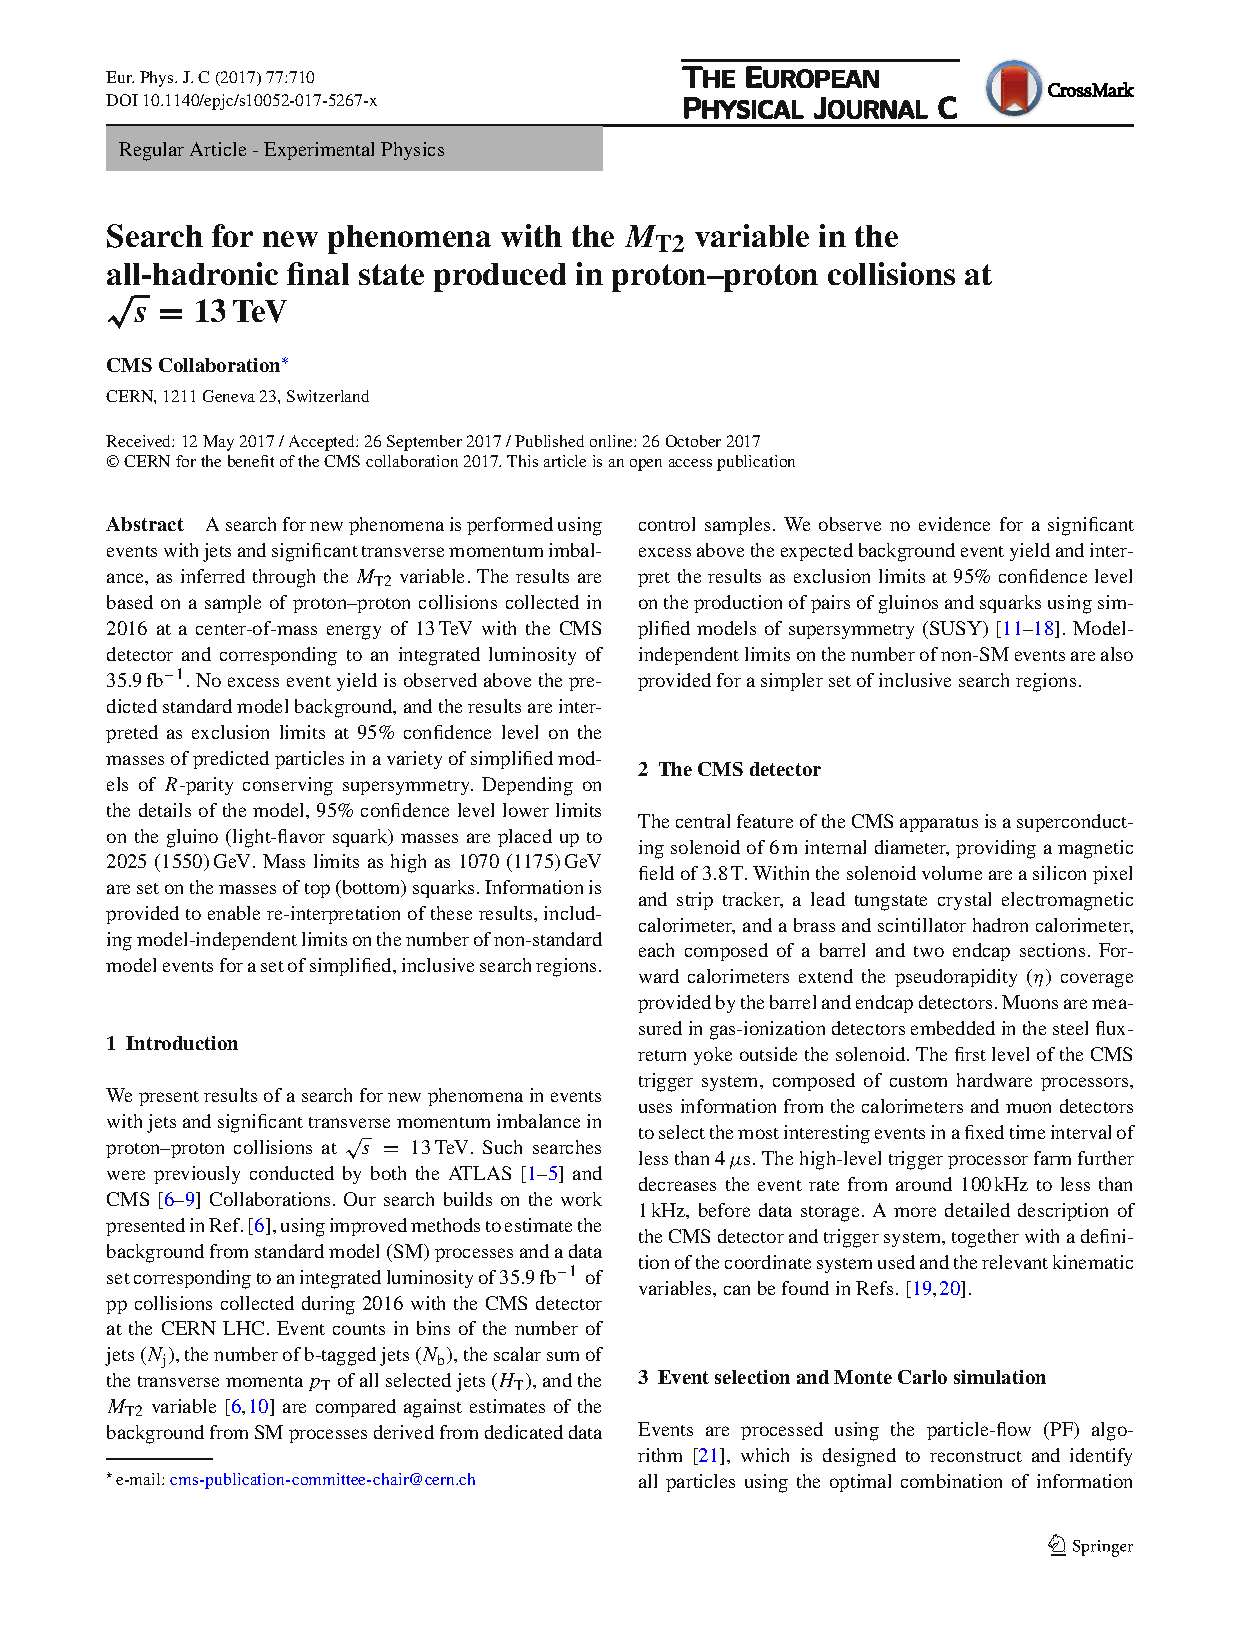
\includepdf[pages={1,2,3}]{Articulos/ArticulosReducidos/Investigacion_Publicaciones_Search_for_new_phenomena_with_the_MT2_variable_in_the_all-hadroni.pdf}
\subsubsection{Search for supersymmetry in multijet events with missing transverse momentum in proton-proton collisions at 13 TeV}
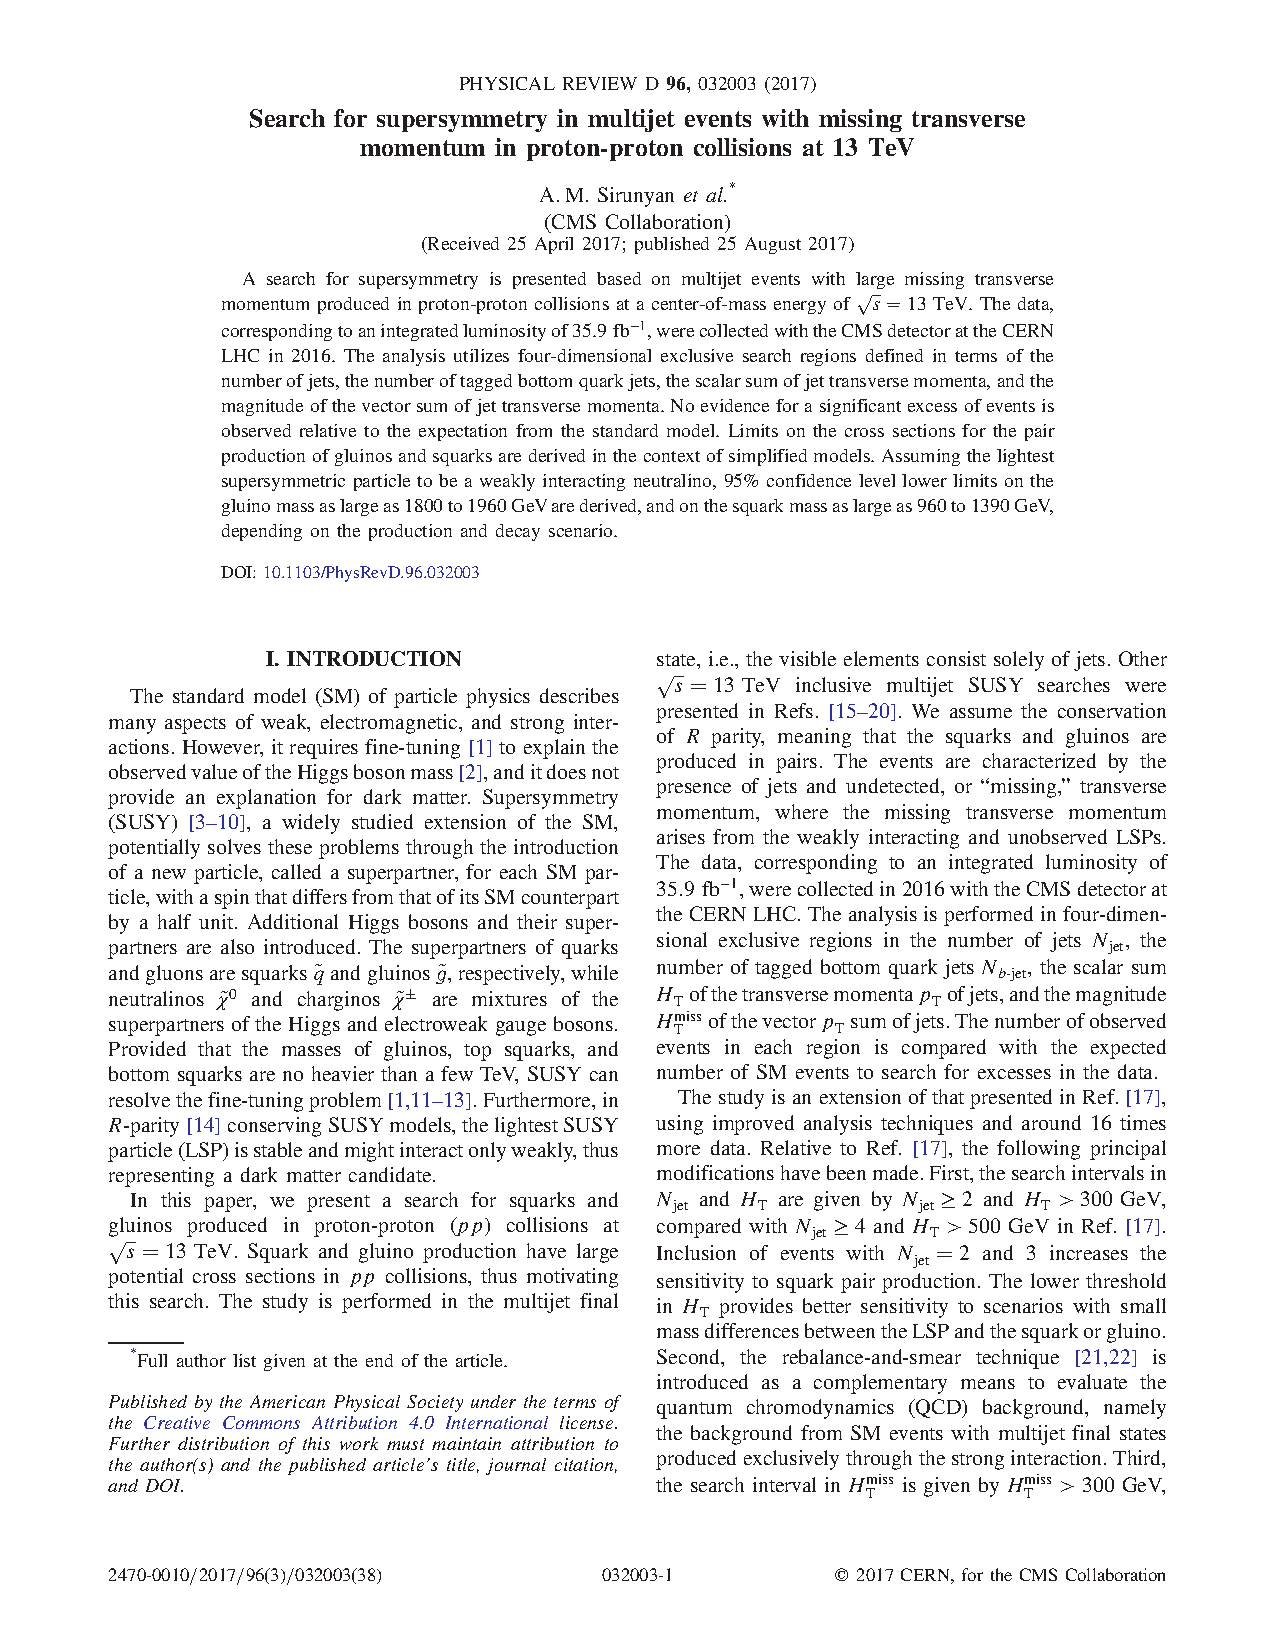
\includepdf[pages={1,2,3}]{Articulos/ArticulosReducidos/Investigacion_Publicaciones_Search_for_supersymmetry_in_multijet_events_with_missing_transver.pdf}
\subsubsection{Search for Supersymmetry in pp Collisions at sqrt s 13 TeV in the Single-Lepton Final State Using the Sum of Masses of Large-Radius Jets}
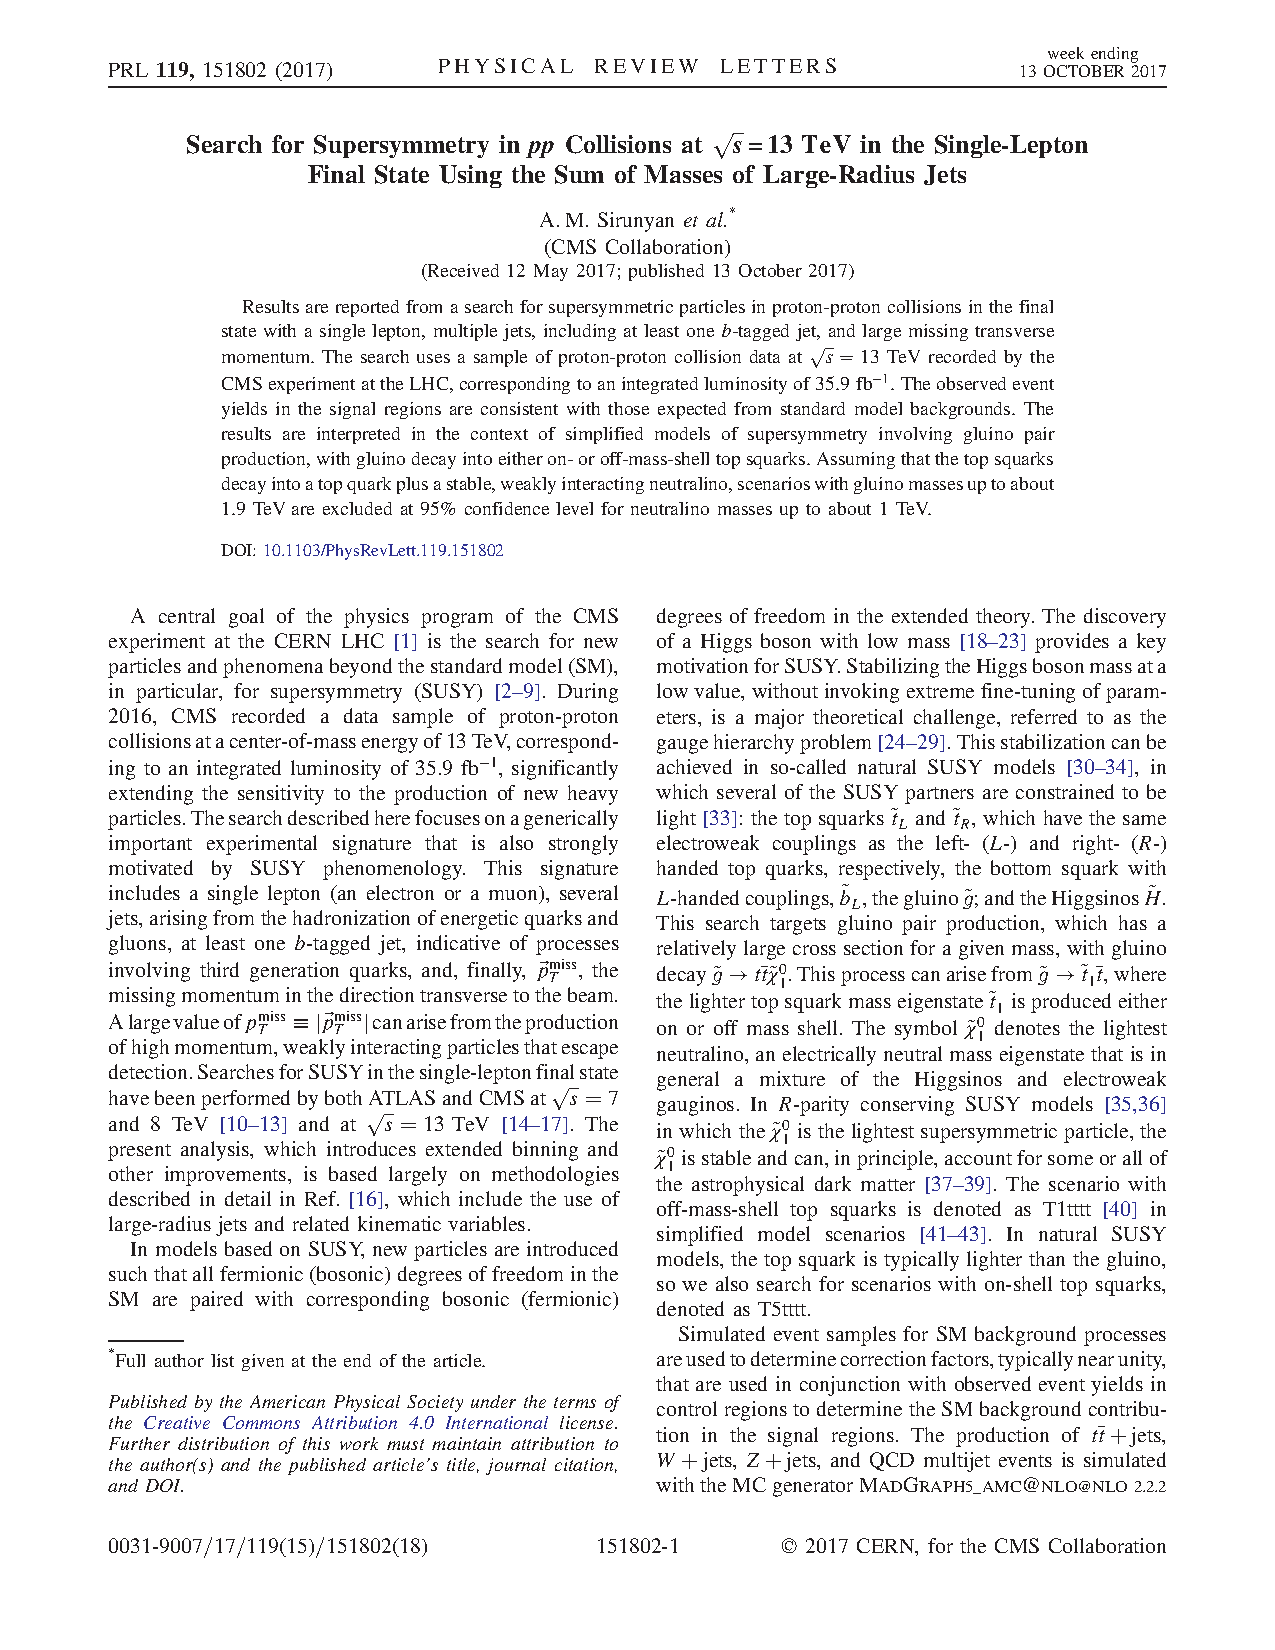
\includepdf[pages={1,2,3}]{Articulos/ArticulosReducidos/Investigacion_Publicaciones_Search_for_Supersymmetry_in_pp_Collisions_at_sqrt_s_13_TeV_in_the.pdf}
\subsection{A new boson with a mass of 125 GeV observed with the CMS Experiment at the Large Hadron Collider}
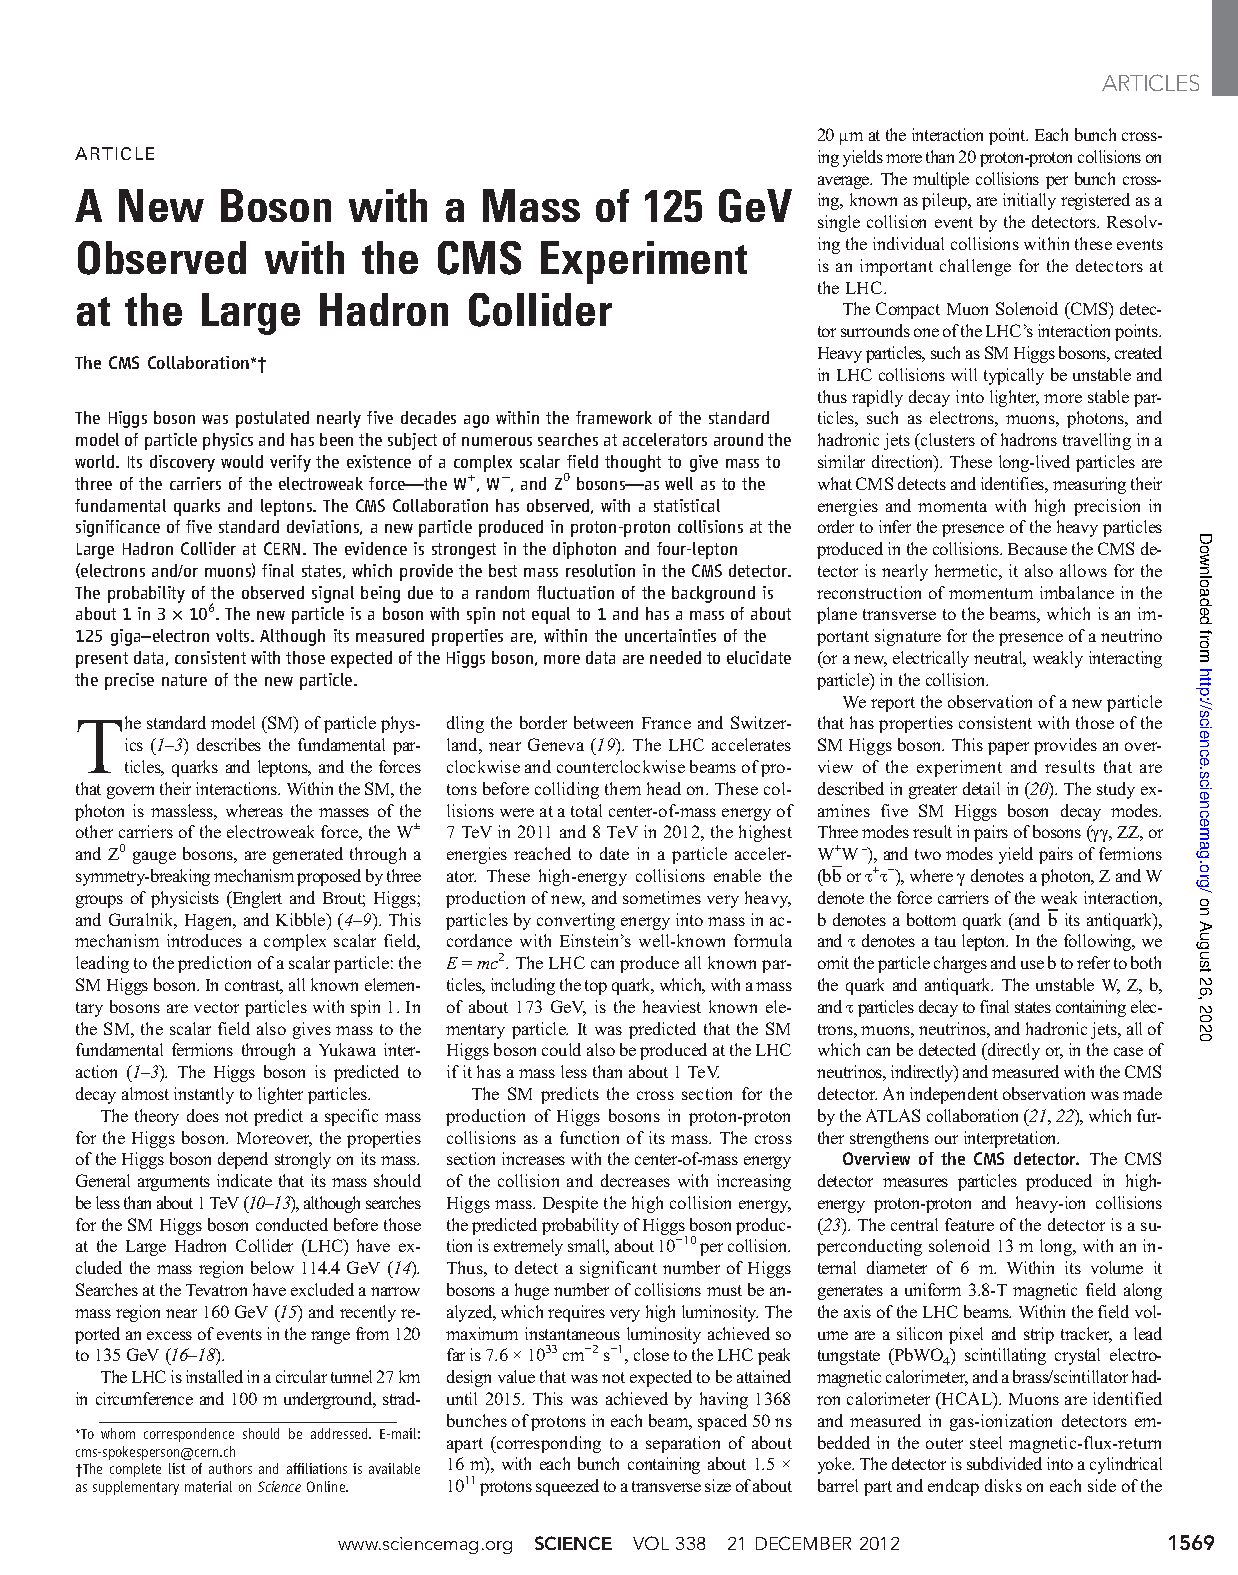
\includepdf[pages={1,2}]{Articulos/ArticulosReducidos/Investigacion_Publicaciones_A_New_Boson_With_A_Mass_Of_125GeV.pdf}
\subsection{Observation of a new boson with a mass of 125 GeV with the CMS experiment at the LHC }
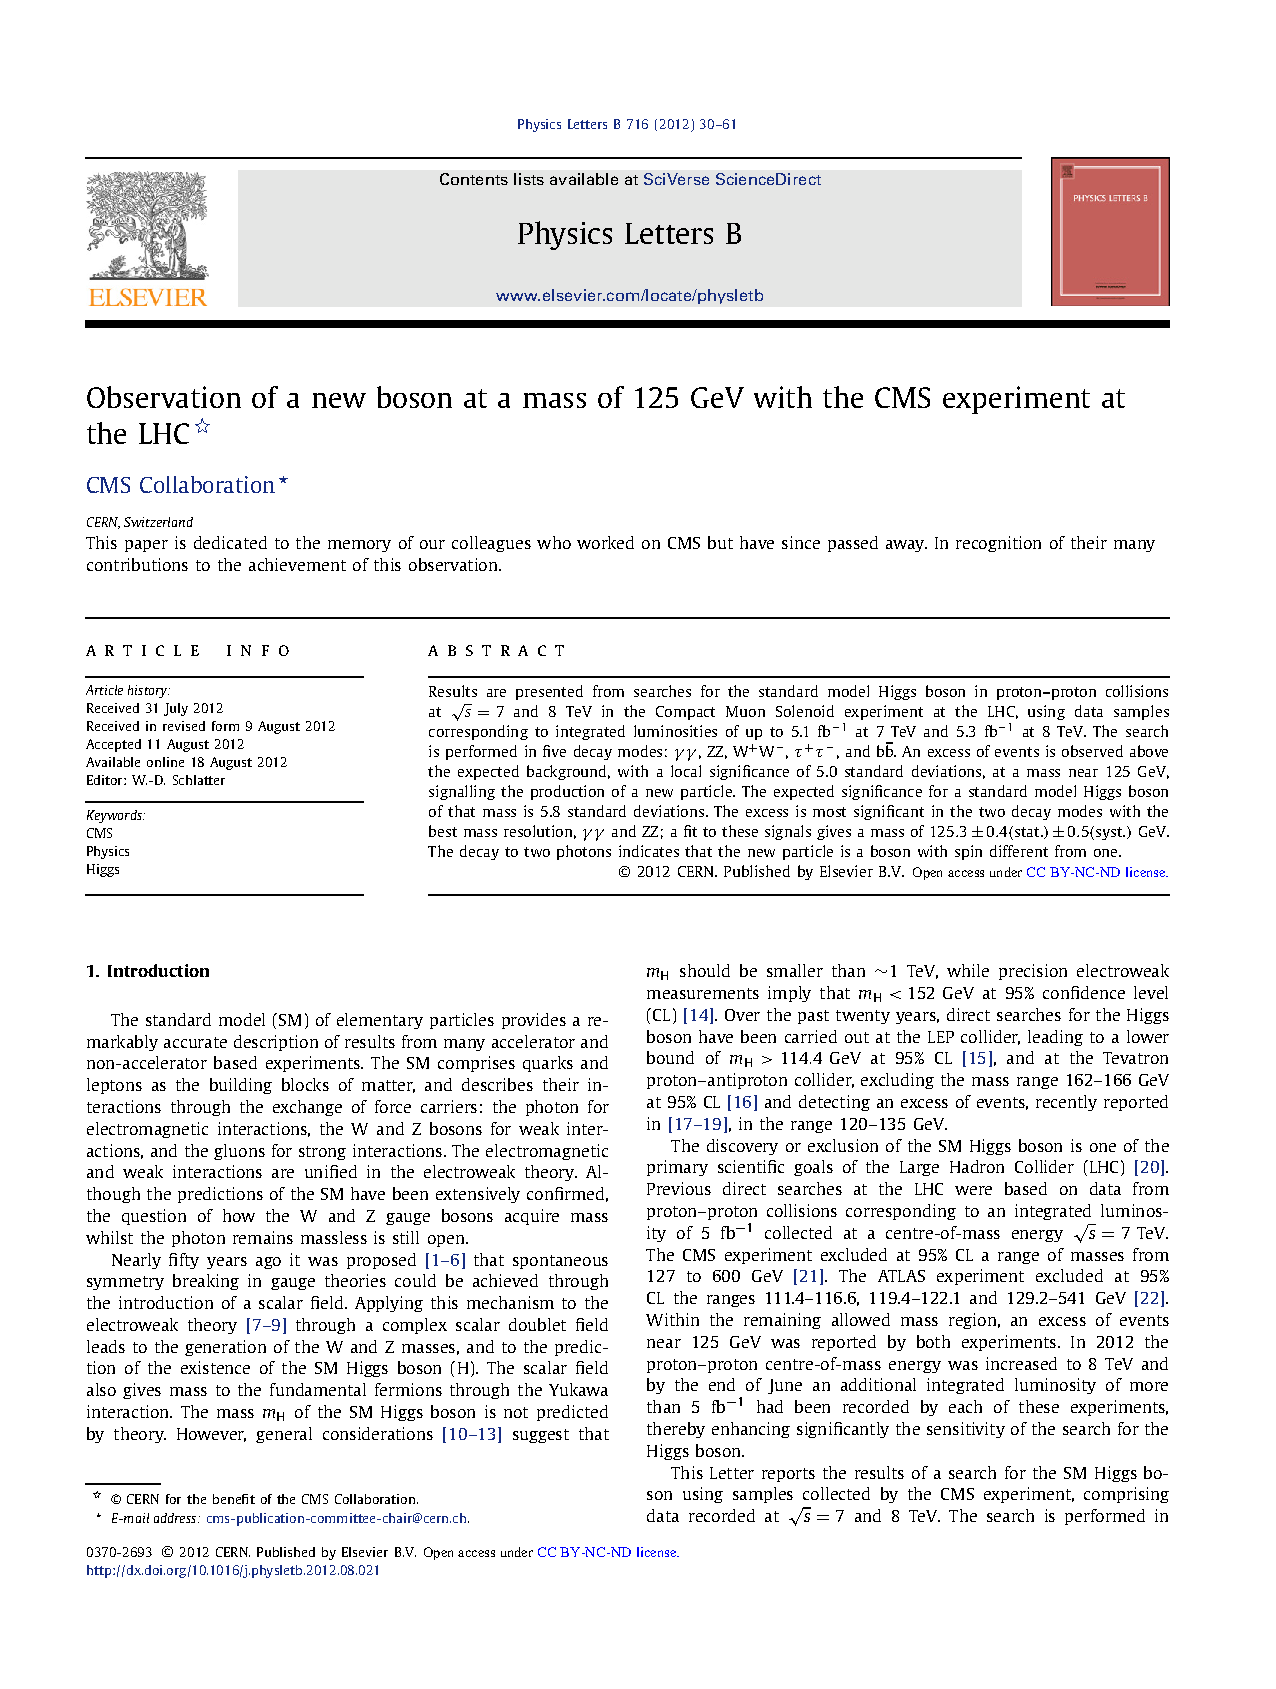
\includepdf[pages={1,2,3}]{Articulos/ArticulosReducidos/Investigacion_Publicaciones_Observation_Of_A_New_Boson.pdf}
\subsubsection{Search for electroweak production of charginos and neutralinos in WH events in proton-proton collisions at sqrt s 13 TeV}
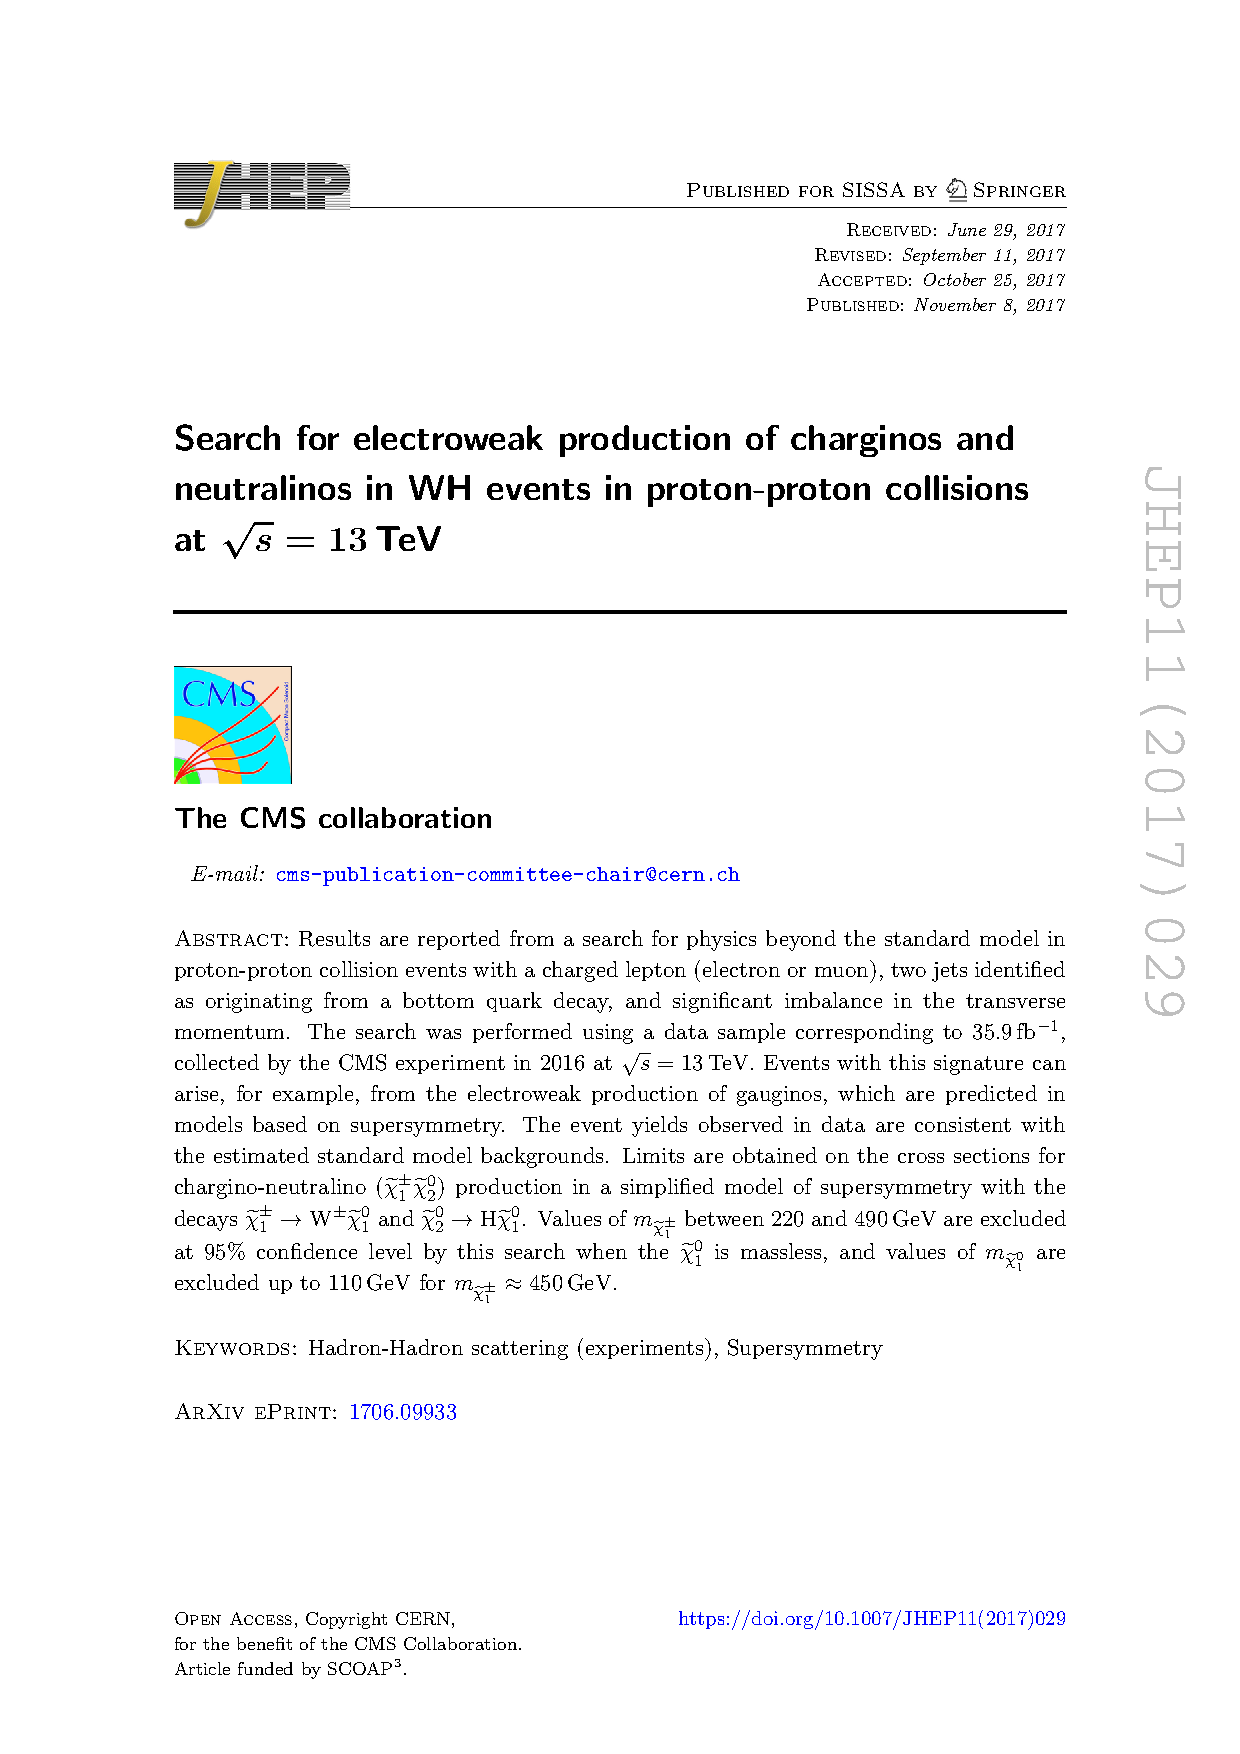
\includepdf[pages={1,2,3}]{Articulos/ArticulosReducidos/Investigacion_Publicaciones_Search_for_electroweak_production_of_charginos_and_neutralinos_in.pdf}
\subsubsection{A search for new phenomena in pp collisions at sqrt s 13 TeV in final states with missing transverse momentum and at least one jet using the aT variable}
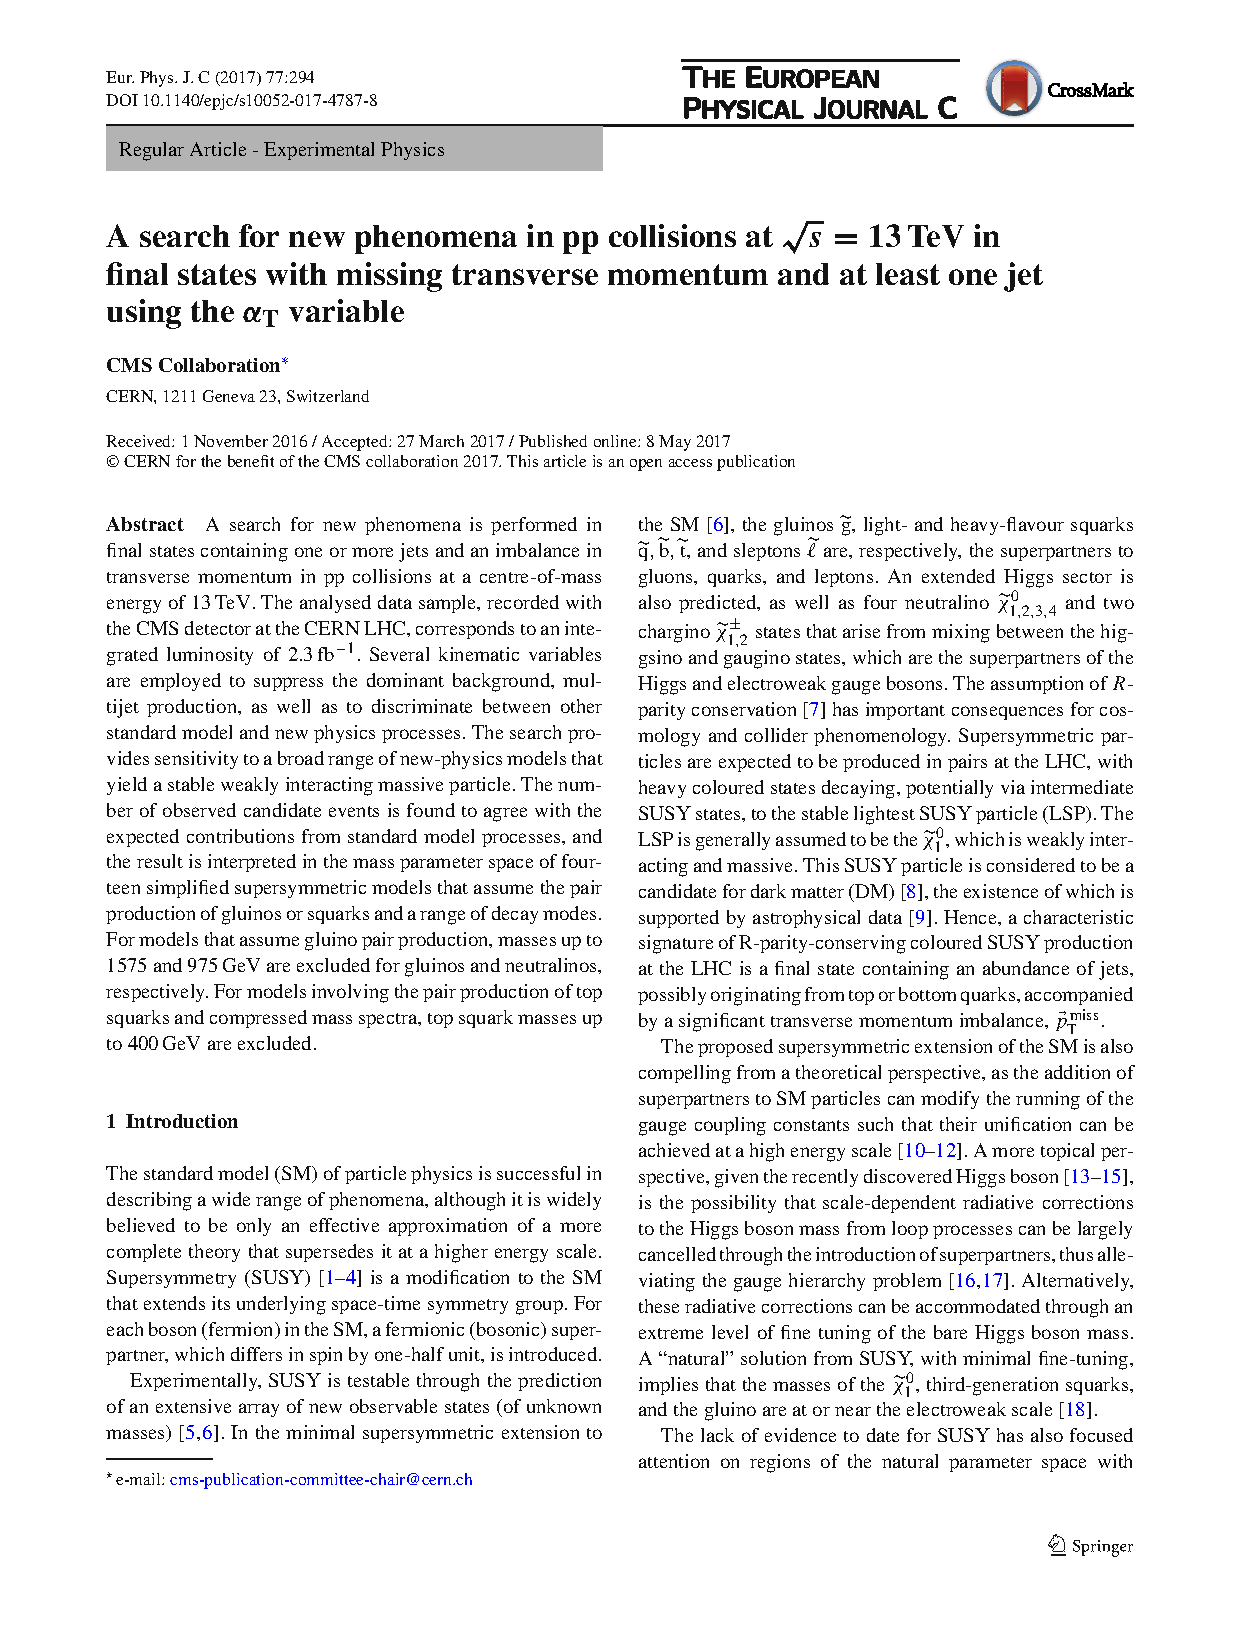
\includepdf[pages={1,2,3}]{Articulos/ArticulosReducidos/Investigacion_Publicaciones_A_search_for_new_phenomena_in_pp_collisions_at_sqrt_s_13_TeV_in_f.pdf}
\subsubsection{Jet energy scale and resolution in the CMS experiment in pp collisions at 8 TeV}
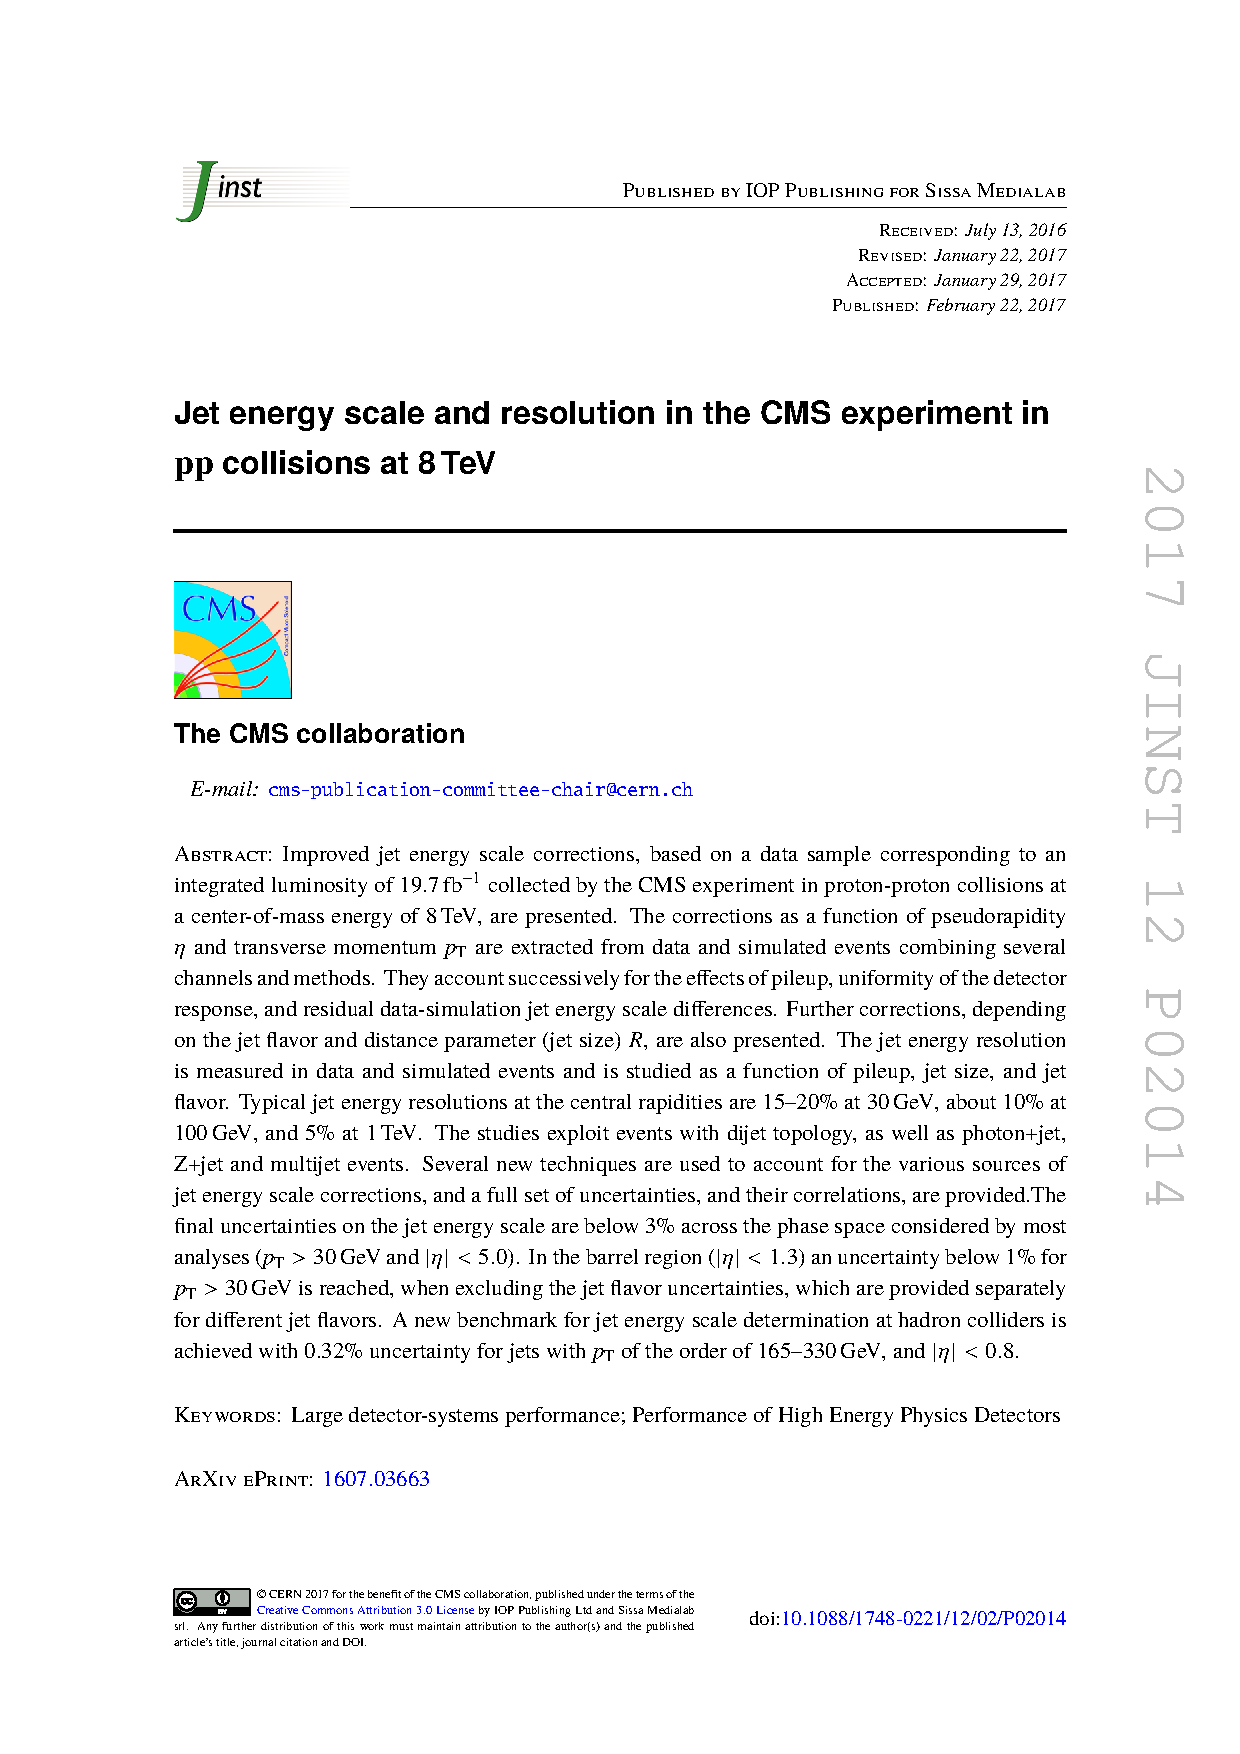
\includepdf[pages={1,2,3}]{Articulos/ArticulosReducidos/Investigacion_Publicaciones_Jet_Energy_Resolution_In_The_CMS_Experiment_In_PP_Collisions.pdf}
\subsubsection{The CMS Trigger System}
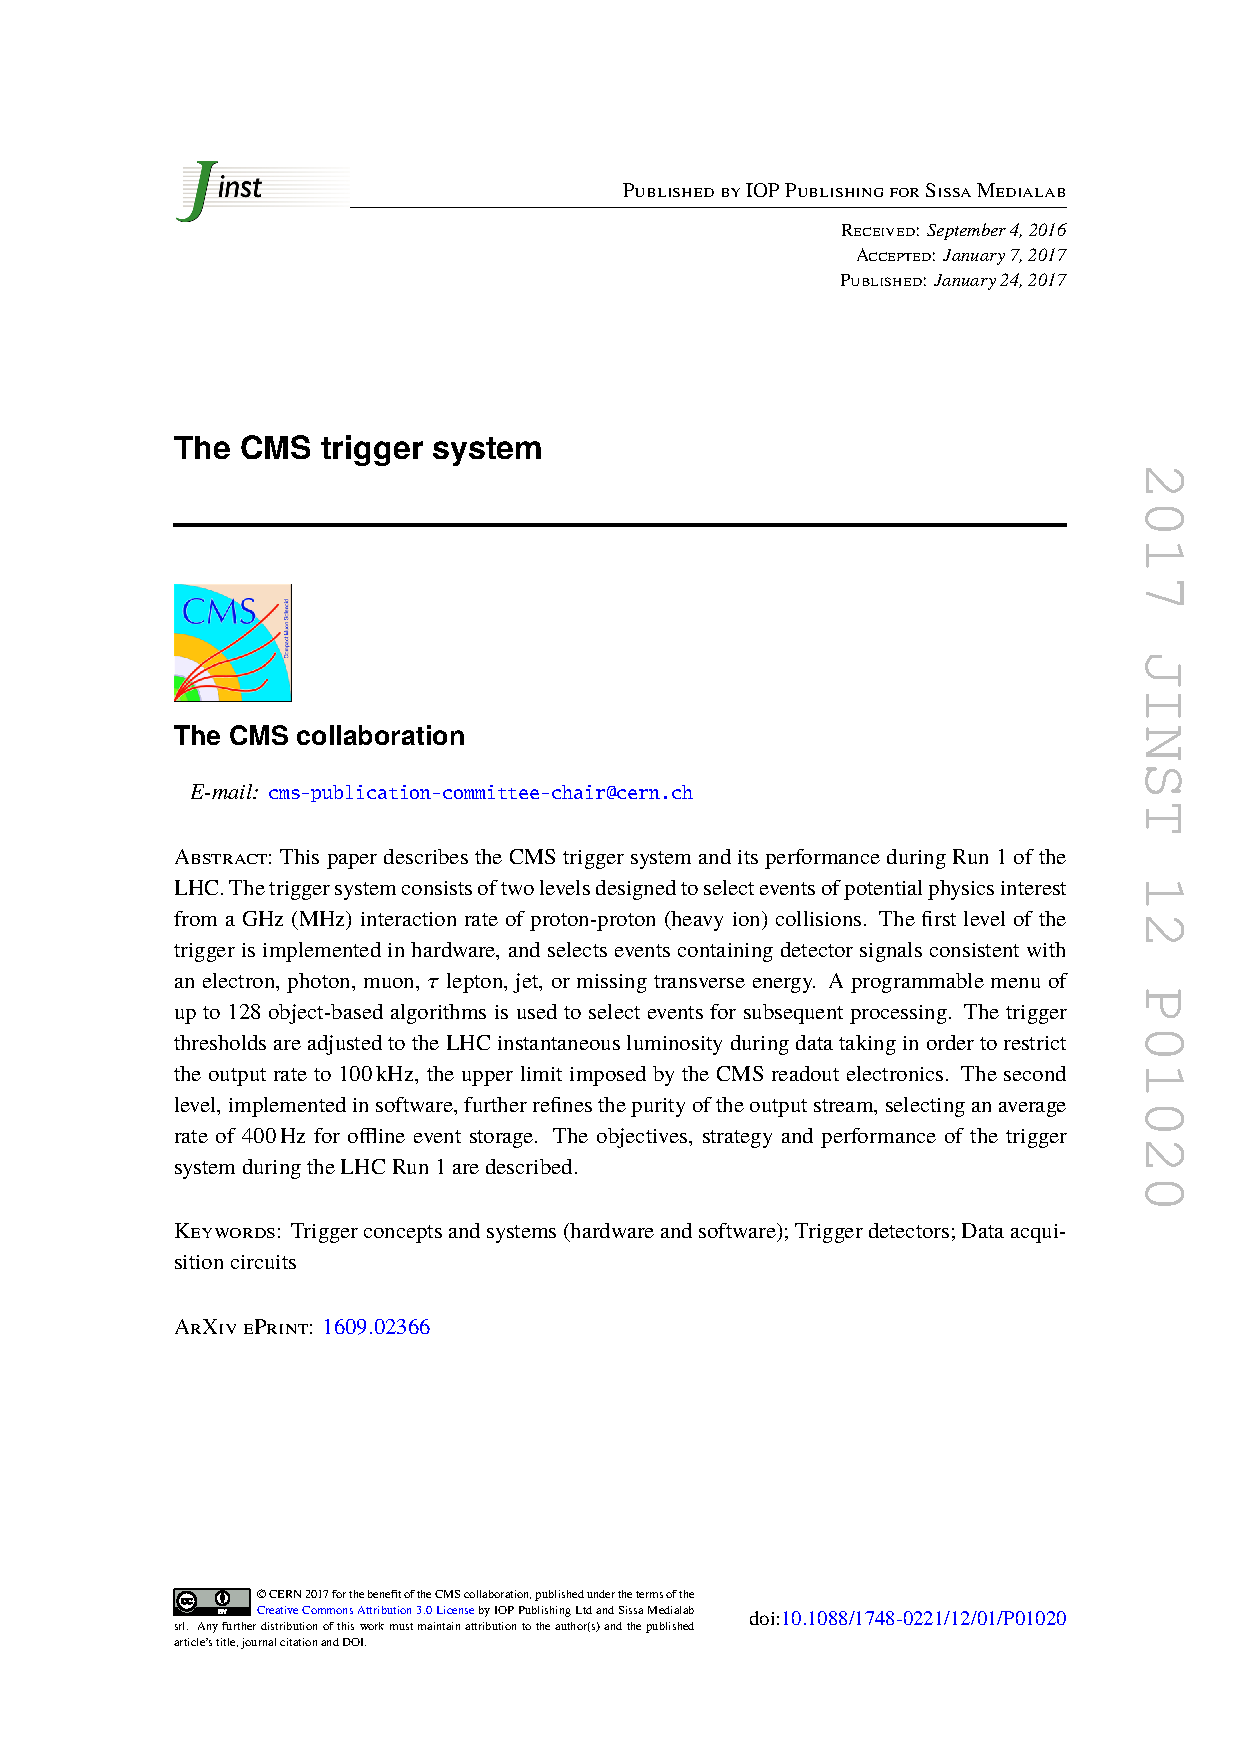
\includepdf[pages={1,2,3}]{Articulos/ArticulosReducidos/Investigacion_Publicaciones_The_CMS_Trigger_System.pdf}
\subsubsection{Search for new phenomena in final states with two opposite-charge same-flavor leptons jets and missing transverse momentum in pp collisions at sqrt s 13 TeV}
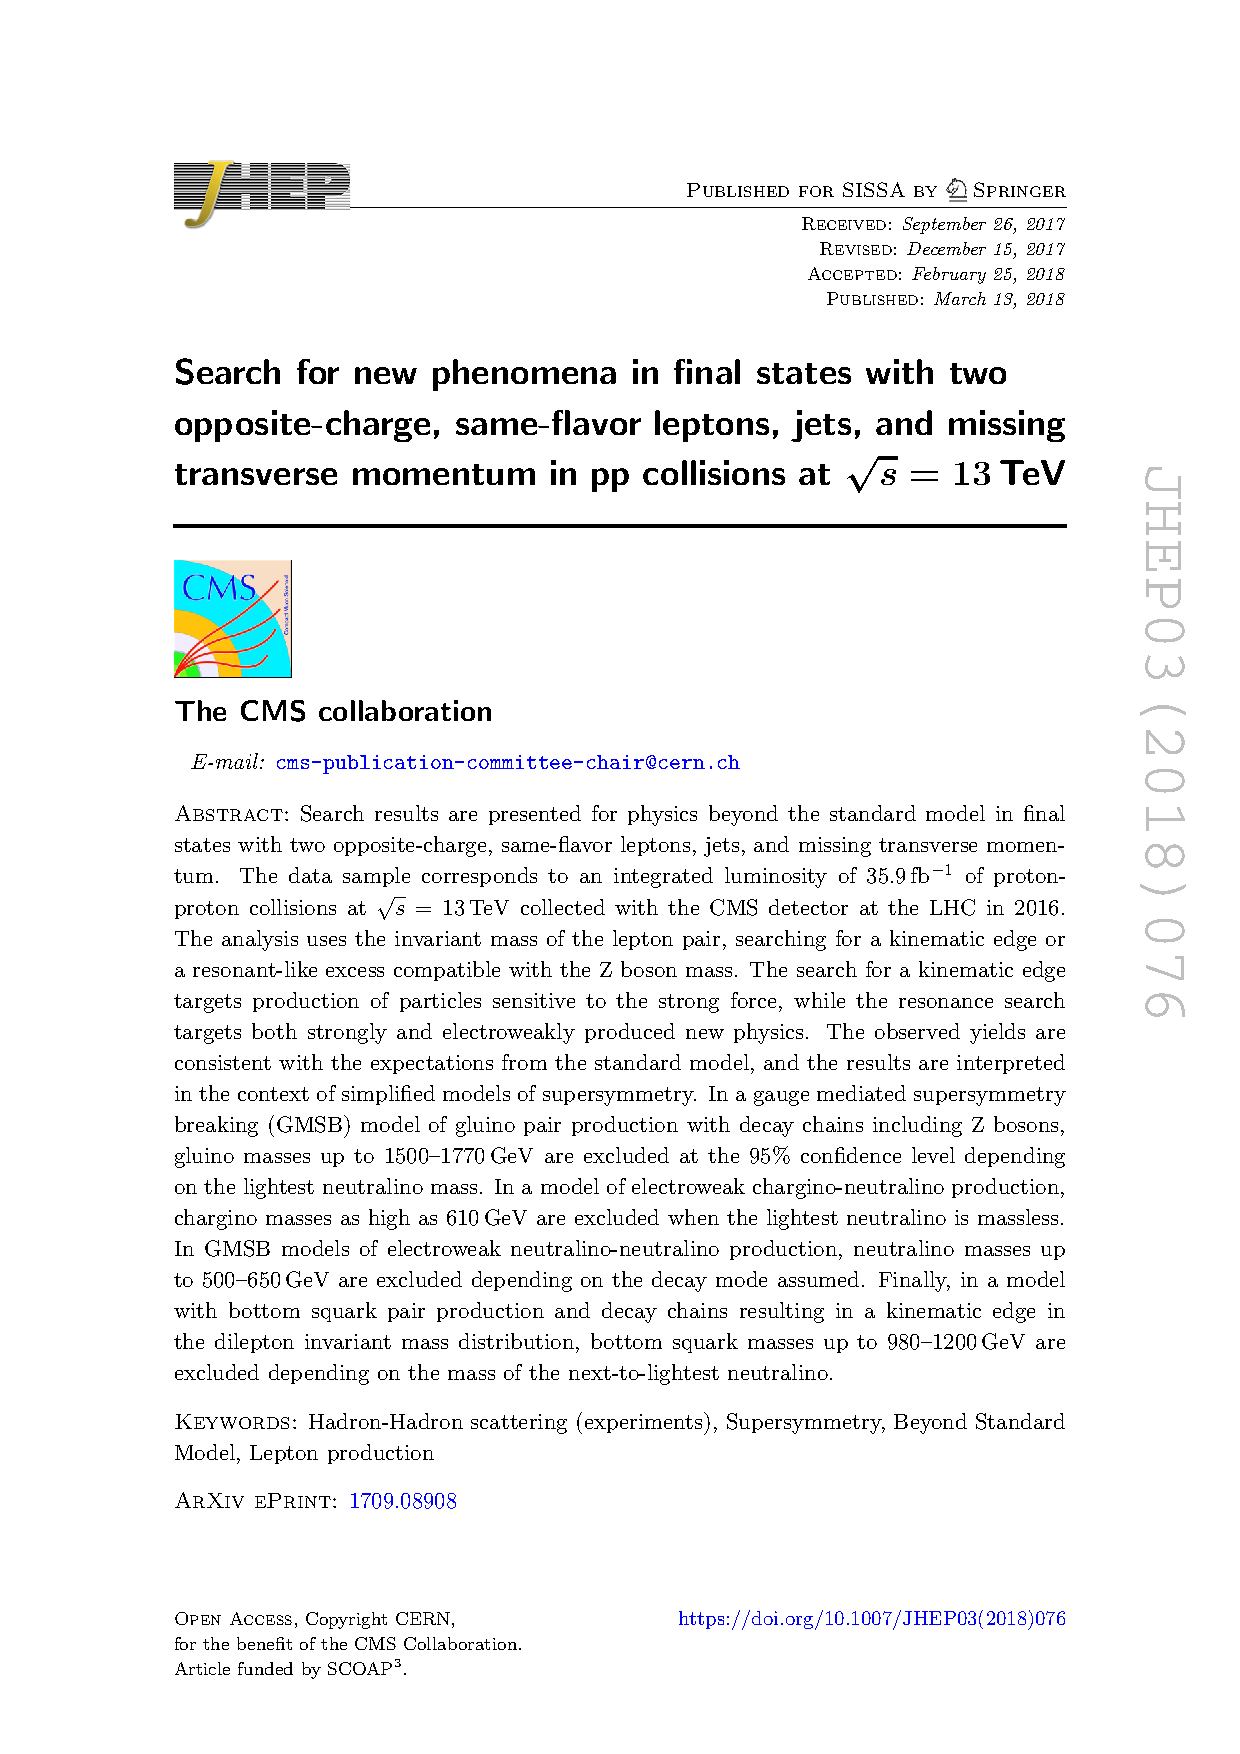
\includepdf[pages={1,2,3}]{Articulos/ArticulosReducidos/Investigacion_Publicaciones_Search_for_new_phenomena_in_final_states_with_two_opposite-charge.pdf}
\subsubsection{Searches for pair production of charginos and top squarks in final states with two oppositely charged leptons in proton-proton collisions at sqrt s 13 TeV}
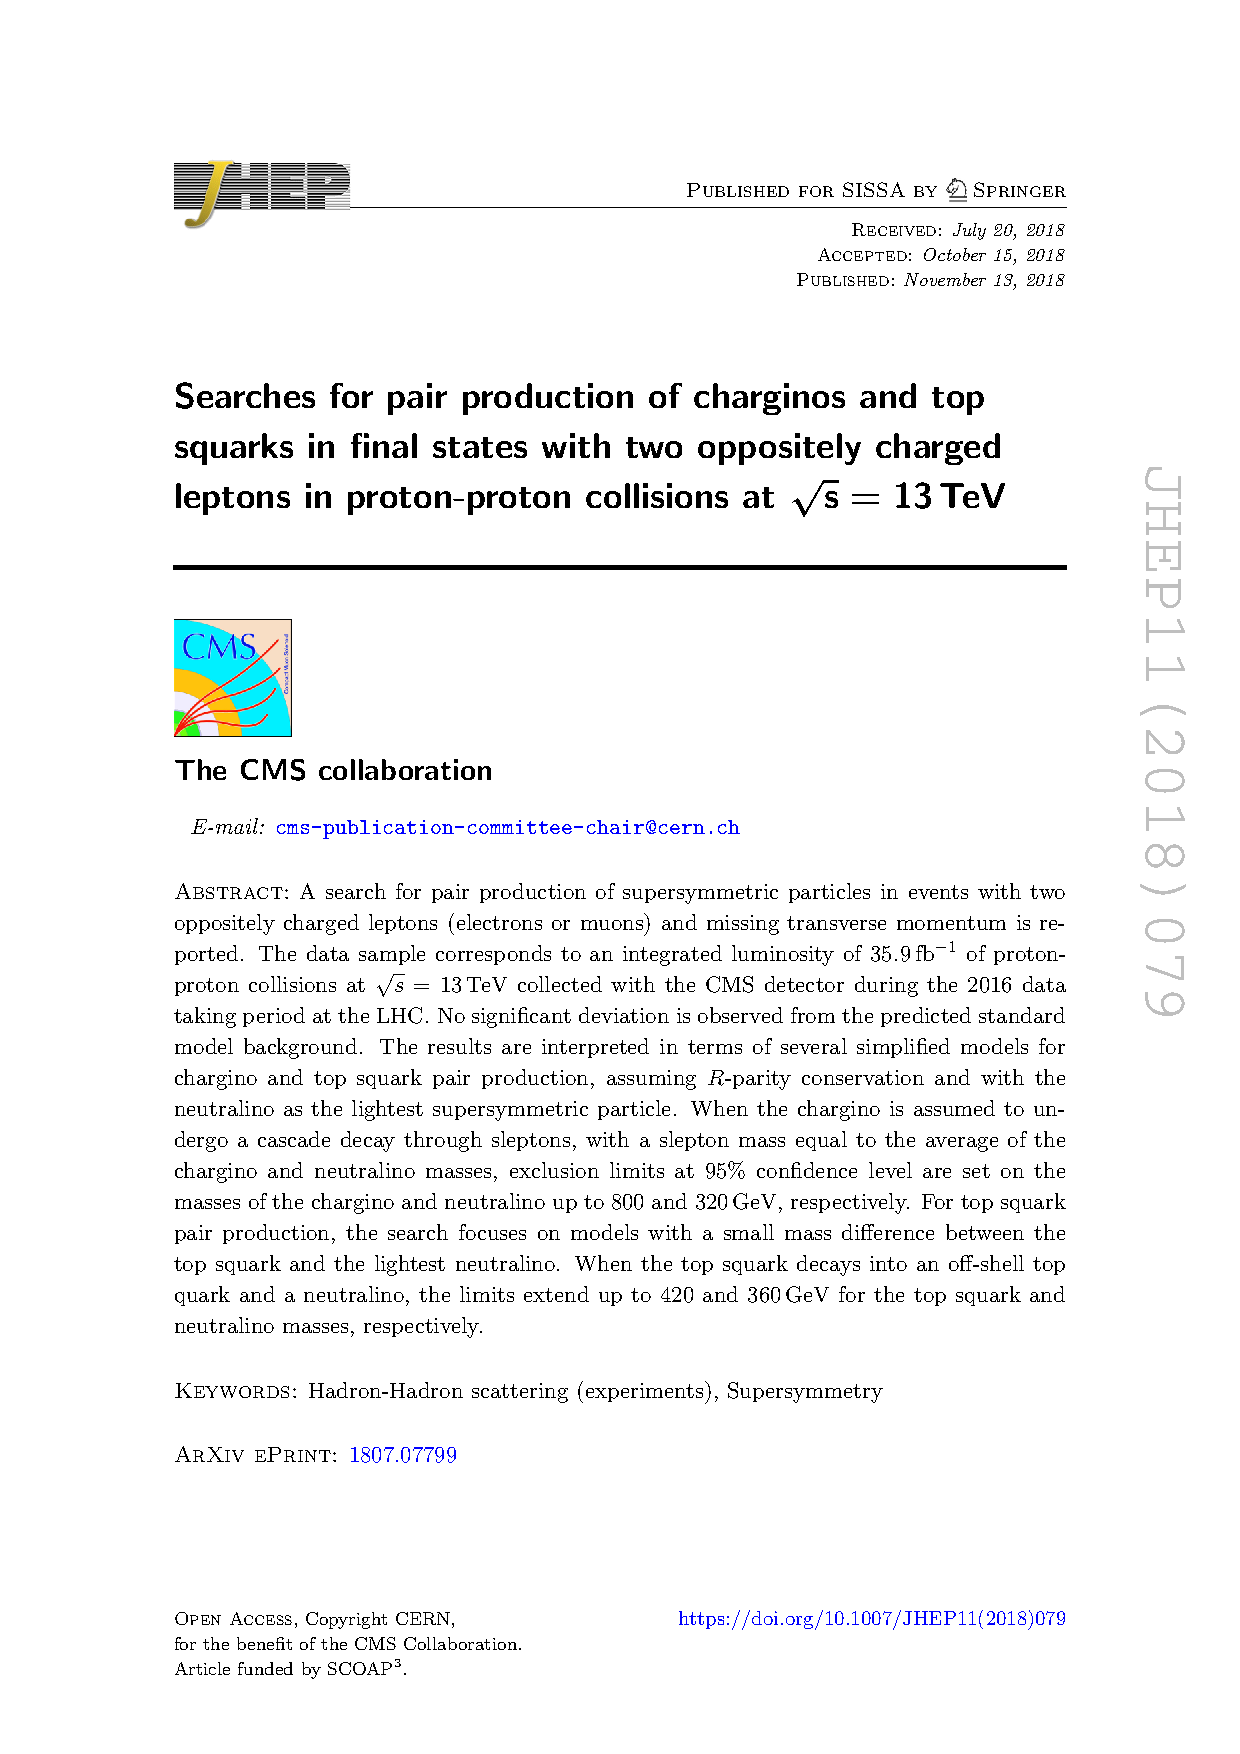
\includepdf[pages={1,2,3}]{Articulos/ArticulosReducidos/Investigacion_Publicaciones_Searches_for_pair_production_of_charginos_and_top_squarks_in_fina.pdf}
\subsubsection{Non-destructive testing of industrial equipment using muon radiography}
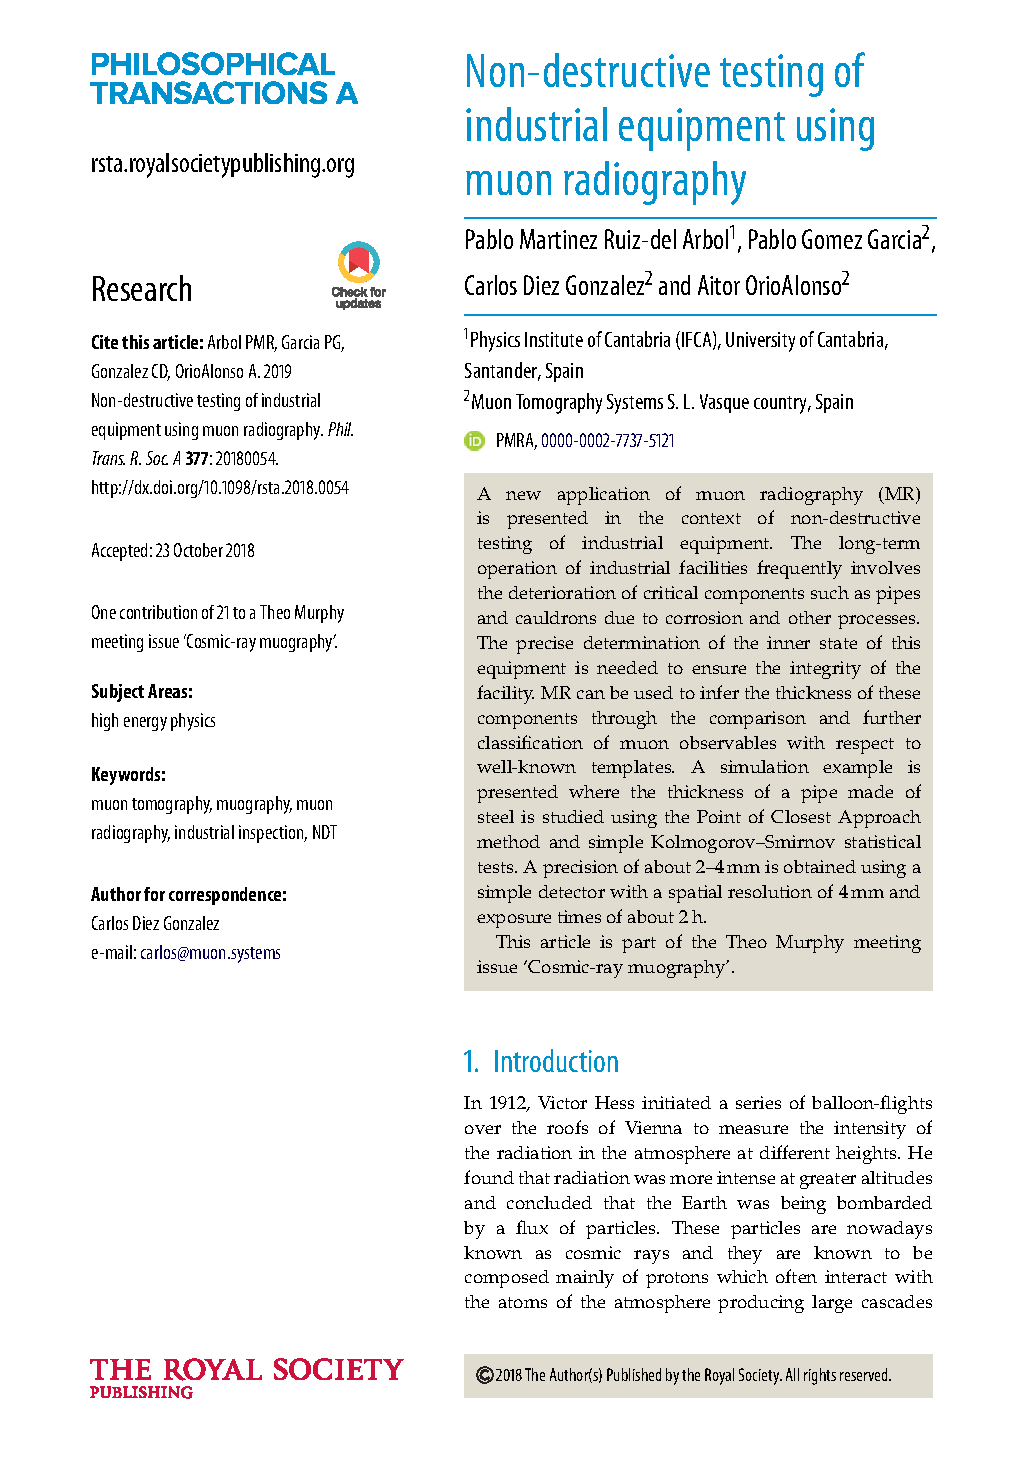
\includepdf[pages={1,2}]{Articulos/ArticulosReducidos/Investigacion_Publicaciones_Non-destructive_testing_of_industrial_equipment_using_muon_radiog.pdf}
\subsubsection{Search for the pair production of third-generation squarks with two-body decays to a bottom or charm quark and a nuetralino in proton-proton collisions at sqrt s 13 TeV}
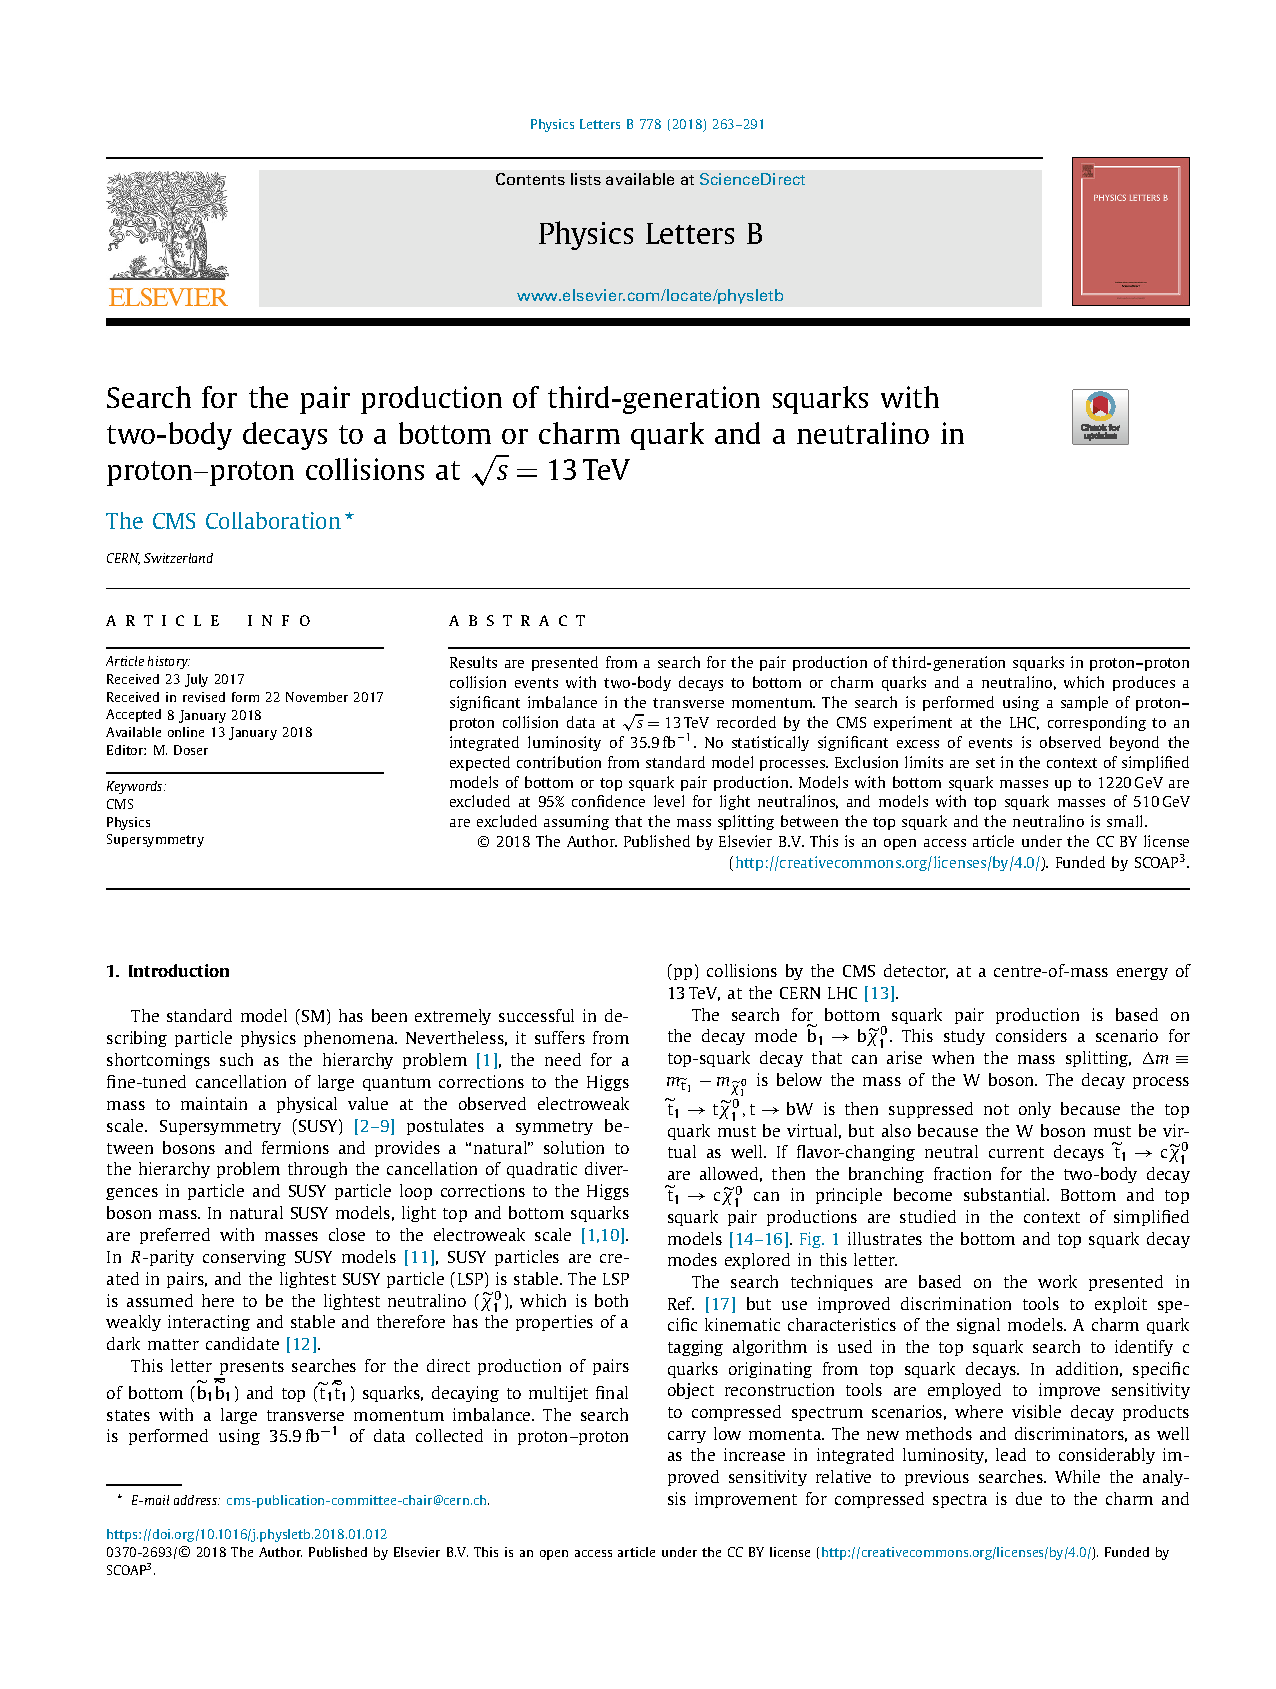
\includepdf[pages={1,2,3}]{Articulos/ArticulosReducidos/Investigacion_Publicaciones_Search_for_the_pair_production_of_third-generation_squarks_with_t.pdf}
\subsubsection{Search for electroweak production of charginos and neutralinos in multilepton final states in proton-proton collisions at sqrt s 13 TeV}
\includepdf[pages={1,2,3}]{Articulos/ArticulosReducidos/Investigacion_Publicaciones_Search_for_electroweak_production_of_charginos_and_neutralinos_in_2.pdf}
\subsubsection{Search for supersymmetry in proton-proton collisions at sqrt s 13 TeV using identified top quarks}
\includepdf[pages={1,2,3}]{Articulos/ArticulosReducidos/Investigacion_Publicaciones_Search_for_supersymmetry_in_proton-proton_collisions_at_sqrt_s_13.pdf}
\subsubsection{Search for top squarks and dark matter particles in opposite-charge dilepton final states at sqrt s 13 TeV}
\includepdf[pages={1,2,3}]{Articulos/ArticulosReducidos/Investigacion_Publicaciones_Search_for_top_squarks_and_dark_matter_particles_in_opposite-char.pdf}
\subsubsection{Search for supersymmetry in events with a tau lepton pair and missing transverse momentum in proton-proton collisions at sqrt s 13 TeV}
\includepdf[pages={1,2,3}]{Articulos/ArticulosReducidos/Investigacion_Publicaciones_Search_for_supersymmetry_in_events_with_a_tau_lepton_pair_and_mis.pdf}
\subsubsection{Combined search for electroweak production of charginos and neutralinos in proton-proton collisions at sqrt s 13 TeV}
\includepdf[pages={1,2,3}]{Articulos/ArticulosReducidos/Investigacion_Publicaciones_Combined_search_for_electroweak_production_of_charginos_and_neutr.pdf}
\subsubsection{Search for dark matter particles produced in association with a top quark pair at sqrt s 13 TeV}
\includepdf[pages={1,2,3}]{Articulos/ArticulosReducidos/Investigacion_Publicaciones_Search_for_dark_matter_particles_produced_in_association_with_a_t.pdf}
\subsubsection{Search for supersymmetric partners of electrons and muons in proton–proton collisions at sqrt s 13TeV}
\includepdf[pages={1,2,3}]{Articulos/ArticulosReducidos/Investigacion_Publicaciones_Search_for_supersymmetric_partners_of_electrons_and_muons_in_prot.pdf}
\subsubsection{Search for the pair production of light top squarks in the emu final state in proton-proton collisions at sqrt s 13 TeV}
\includepdf[pages={1,2,3}]{Articulos/ArticulosReducidos/Investigacion_Publicaciones_Search_for_the_pair_production_of_light_top_squarks_in_the_emu_fi.pdf}
\subsubsection{Search for supersymmetry in final states with two oppositely charged same-flavor leptons and missing transverse momentum in proton-proton collisions at sqrt(s) = 13 TeV}
\includepdf[pages={1,2,3}]{Articulos/ArticulosReducidos/Investigacion_Publicaciones_Search_For_Supersymmetry_In_Final_States_with_two.pdf}
\subsubsection{Machine Learning Methods for the Prediction of the Inclusion Content of Clean Steel Fabricated by Electric Arc Furnace and Rolling}
\includepdf[pages={1,2}]{Articulos/ArticulosReducidos/Investigacion_Publicaciones_Machine_Learning_Methods_For_The_Prediction.pdf}



\subsection{Publicaciones científicas no indexadas en JCR}

\subsubsection{Muon Reconstruction in the CMS Detector}
\includepdf[pages={1,2}]{ArticulosNoJCR/ArticulosReducidos/Investigacion_PublicacionesNoJCR_Muon_Reconstruction_in_the_CMS.pdf}

\subsubsection{Una visión global de la pandemia Covid-19: qué sabemos y qué estamos investigando desde el CSIC}
\includepdf[pages={1,2}]{ArticulosNoJCR/ArticulosReducidos/Investigacion_PublicacionesNoJCR_INFORME_Cov19_PTI_Salud_Global_CSIC_v3.pdf}



\subsection{Libros y capítulos de libros}
\subsubsection{A MIP Timing Detector for the CMS Phase-2 Upgrade: Technical Design Report}
\includepdf[pages={1,2,3,4,5}]{Libros/Investigacion_Libros_A_MIP_Timing_Detector_for_the_CMS_Phase2.pdf}


\subsection{Creaciones artísticas y profesionales}

\subsection{Contribuciones a congresos y conferencias científicas}

\subsubsection{The CMS Muon System Alignment}
\includepdf[pages=-]{Conferencias/Investigacion_Congresos_The_CMS_Muon_System_Alignment.pdf}
\subsubsection{A software and computing prototype for CMS muon system alignment}
\includepdf[pages=-]{Conferencias/Investigacion_Congresos_A_software_and_computing_prototype.pdf}
\subsubsection{THE CMS MUON SYSTEM ALIGNMENT FIRST RESULTS FROM COMMISSIONING RUNS}
\includepdf[pages=-]{Conferencias/Investigacion_Congresos_THE_CMS_MUON_SYSTEM_ALIGNMENT_FIRST_RESULTS_FROM_COMMISSIONING_RU.pdf}
\subsubsection{Muon Alignment in ATLAS and CMS}
\includepdf[pages=-]{Conferencias/Investigacion_Congresos_Muon_Alignment_In_ATLAS_AND_CMS.pdf}
\subsubsection{Commissioning and performance of the CMS detector}
\includepdf[pages=-]{Conferencias/Investigacion_Congresos_Commissioning_And_Performance_Of_The_CMS_Detector.pdf}
\subsubsection{SUSY SEARCHES IN THE Z JETS MET FINAL STATE IN 7 TEV PP COLLISIONS WITH THE JET Z BALANCE METHOD}
\includepdf[pages=-]{Conferencias/Investigacion_Congresos_SUSY_SEARCHES_IN_THE_Z_JETS_MET_FINAL_STATE_IN_7_TEV_PP_COLLISION.pdf}
\subsubsection{SEARCHES FOR SUSY IN EVENTS WITH TWO OR MORE LEPTONS AT CMS}
\includepdf[pages=-]{Conferencias/Investigacion_Congresos_SEARCHES_FOR_SUSY_IN_EVENTS_WITH_TWO_OR_MORE_LEPTONS_AT_CMS.pdf}
\subsubsection{SEARCH FOR BEYOND THE STANDARD MODEL PHYSICS IN MULTILEPTONIC AND PHOTONIC FINAL STATES WITH THE CMS DETECTOR}
\includepdf[pages=-]{Conferencias/Investigacion_Congresos_SEARCH_FOR_BEYOND_THE_STANDARD_MODEL_PHYSICS_IN_MULTILEPTONIC_AND.pdf}
\subsubsection{Review of Supersymmetry Searches at 13 TeV with the CMS experiment}
\includepdf[pages=-]{Conferencias/Investigacion_Congresos_Review_of_Supersymmetry_Searches_at_13_TeV_with_the_CMS_experimen.pdf}
\subsubsection{Searches for BSM physics in the 2 leptons y MET final state}
\includepdf[pages=-]{Conferencias/Investigacion_Congresos_Searches_for_BSM_physics_in_the_2_leptons_y_MET_final_state.pdf}
\subsubsection{Dark Matter at the LHC}
\includepdf[pages=-]{Conferencias/Investigacion_Congresos_Dark_Matter_at_the_LHC.pdf}
\subsubsection{Application of muon tomography to the industry}
\includepdf[pages=-]{Conferencias/Investigacion_Congresos_Application_of_muon_tomography_to_the_industry.pdf}
\subsubsection{Precision timing with the CMS MIP Timing Detector}
\includepdf[pages=-]{Conferencias/Investigacion_Congresos_Precision_timing_with_the_CMS_MIP_Timing_Detector.pdf}
\subsubsection{Muography applied to the preventive maintenance of industrial equipment}
\includepdf[pages=-]{Conferencias/Investigacion_Congresos_Muography_applied_to_the_preventive_maintenance_of_industrial_equ.pdf}
\subsubsection{COMCHA: Computing Challanges for the HLLHC and beyond}
\includepdf[pages=-]{Conferencias/Investigacion_Congresos_COMCHA_Computing_Challanges_for_the_HLLHC_and_beyond.pdf}
\subsubsection{Timing for the CMS PhaseII Upgrade}
\includepdf[pages=-]{Conferencias/Investigacion_Congresos_Timing_for_the_CMS_PhaseII_Upgrade.pdf}
\subsubsection{Summary of SUSY searches}
\includepdf[pages=-]{Conferencias/Investigacion_Congresos_COMHEP.pdf}

\subsection{Contribuciones a seminarios}

\subsubsection{CMS SUSY SEARCHES AT 13 TEV}
\includepdf[pages=-]{Seminarios/Investigacion_Seminarios_CMS_SUSY_SEARCHES_AT_13_TEV.pdf}

\subsubsection{Comparación de estrategias de control epidemiológico basadas en simulaciones con agentes autónomos y énfasis en el impacto del uso de aplicaciones de rastreo}
\includepdf[pages=-]{Seminarios/Investigacion_Seminarios_Comparacion_de_estrategias_de_control.pdf}

\subsubsection{MAINTENANCE OF CRITICAL INDUSTRIAL EQUIPMENT USING COSMIC MUON RADIATION (Zurich)}
\includepdf[pages=-]{Seminarios/Investigacion_Seminarios_MAINTENANCE_OF_CRITICAL_INDUSTRIAL_EQUIPME.pdf}

\subsubsection{MAINTENANCE OF CRITICAL INDUSTRIAL EQUIPMENT USING COSMIC MUON RADIATION (CIEMAT)}
\includepdf[pages=-]{Seminarios/Investigacion_Seminarios_MAINTENANCE_OF_CRITICAL_INDUSTRIAL_EQUIPME_v2.pdf}

\subsubsection{SUSY SEARCHES WITH TWO OPPOSITE SIGN LEPTONS}
\includepdf[pages=-]{Seminarios/Investigacion_Seminarios_SUSY_SEARCHES_WITH_TWO_OPPOSITE_SIGN_LEPTONS.pdf}



\subsection{Otras méritos asociados a la calidad y difusión de resultados de la actividad investigadora}

\subsubsection{Memorandum de la European Physical Society acerca de la evaluación de Físicos de Partículas Experimentales}
\includepdf[pages=-]{InvestigacionOtrosMeritos/Investigacion_OtrosMeritosCalidadInvestigadora_memorandum-HEP.pdf}

\subsubsection{Carta de Filip Moorgart: coordinador de búsquedas de Supersimetría de CMS}
\includepdf[pages=-]{InvestigacionOtrosMeritos/Investigacion_OtrosMeritosCalidadInvestigadora_LetterFilipMoorgart.pdf}

\subsubsection{Carta de Wolfgang Adam: Physics Coordinator de CMS}
\includepdf[pages=-]{InvestigacionOtrosMeritos/Investigacion_OtrosMeritosCalidadInvestigadora_LetterWolfgangAdam.pdf}


\subsubsection{Otras contribuciones a conferencias cientificas}


\paragraph{Poster: A software and computing prototype for CMS Muon System Alignment}
\includepdf[pages=-]{InvestigacionOtrosMeritos/Investigacion_OtrosMeritosCalidadInvestigadora_Poster_Computing_In_High_Energy.pdf}

\paragraph{Muon Alignment in ATLAS and CMS}
\includepdf[pages=-]{InvestigacionOtrosMeritos/Investigacion_OtrosMeritosCalidadInvestigadora_Detector_Understanding_with_first_lhc.pdf}

\paragraph{Commissioning and Performance of the CMS detector}
\includepdf[pages=-]{InvestigacionOtrosMeritos/Investigacion_OtrosMeritosCalidadInvestigadora_Commissioning_and_Performance.pdf}

\paragraph{CMS workshop at Fermilab, Comité científico}
\includepdf[pages=-]{InvestigacionOtrosMeritos/Investigacion_OtrosMeritosCalidadInvestigadora_SUSY_Workshop_Chicago.pdf}

\paragraph{CMS workshop at Ghent, Comité científico y charla Overview of TBT group}
\includepdf[pages=-]{InvestigacionOtrosMeritos/Investigacion_OtrosMeritosCalidadInvestigadora_SUSY_Workshop_Ghent.pdf}

\paragraph{CMS workshop at Vienna, Comité científico}
\includepdf[pages=-]{InvestigacionOtrosMeritos/Investigacion_OtrosMeritosCalidadInvestigadora_SUSY_Workshop_Viena.pdf}

\paragraph{CMS workshop at Santander, Organizador del workshop}
\includepdf[pages=-]{InvestigacionOtrosMeritos/Investigacion_OtrosMeritosCalidadInvestigadora_SUSY_Workshop_Santander.pdf}



\section{Calidad y número de proyectos y contratos de investigación}

\subsection{Participación en proyectos de investigación y/o en contratos de I+D}

\subsubsection{CENTRO DE PROCESADO DE DATOS PARA EL LHC: TIER-2 PARA EL EXPERIMENTO CMS EN EL IFCA}
\includepdf[pages=-]{Proyectos/Investigacion_Proyectos_CENTRO_DE_PROCESADO_DE_DATOS_PARA_EL_LHC.pdf}

\subsubsection{PARTICIPACIÓN EN EL EXPERIMENTO CMS DEL LHC: RUN2}
\includepdf[pages=-]{Proyectos/Investigacion_Proyectos_PARTICIPACION_EN_EL_EXPERIMENTO_CMS_DEL_LHC_RUN2.pdf}

\subsubsection{HIGH PT PHYSICS WITH CMS AND UPGRADES OF THE CMS BARREL PIXEL DETECTOR}
\includepdf[pages=-]{Proyectos/Investigacion_Proyectos_HIGH_PT_PHYSICS_WITH_CMS_AND_UPGRADES.pdf}

\subsubsection{MEASUREMENTS OF HIGGS BOSON PROPERTIES AND SEARCHES FOR SUPERSYMMETRY WITH CMS}
\includepdf[pages=-]{Proyectos/Investigacion_Proyectos_MEASUREMENTS_OF_HIGGS_BOSON_PROPERTIES.pdf}

\subsubsection{SEARCH FOR NEW PHYSICS MEASUREMENTS OF THE HIGGS BOSON PROPERTIES WITH CMS}
\includepdf[pages=-]{Proyectos/Investigacion_Proyectos_SEARCH_FOR_NEW_PHYSICS_MEASUREMENTS_OF_THE_HIGGS.pdf}

\subsubsection{XDC: EXTREME DATACLOUD}
\includepdf[pages=-]{Proyectos/Investigacion_Proyectos_XDC_EXTREME_DATACLOUD.pdf}

\subsection{Otros méritos relacionados con la calidad y número de proyectos y contratos de investigación}

\subsubsection{Contrato postdoctoral ETH Octubre 2010 - Septiembre 2012}
\includepdf[pages=-]{ContratosInvestigacion/Investigacion_Contratos_ETH_Oct2010_Sept2012.pdf}

\subsubsection{Contrato postdoctoral ETH Octubre 2012 - Septiembre 2013}
\includepdf[pages=-]{ContratosInvestigacion/Investigacion_Contratos_ETH_Oct2012_Sept2013.pdf}

\subsubsection{Contrato postdoctoral ETH Octubre 2013 - Septiembre 2014}
\includepdf[pages=-]{ContratosInvestigacion/Investigacion_Contratos_ETH_Oct2013_Sept2014.pdf}

\subsubsection{Contrato postdoctoral ETH Octubre 2014 - Marzo 2016}
\includepdf[pages=-]{ContratosInvestigacion/Investigacion_Contratos_ETH_Oct2014_Mar2016.pdf}

\subsubsection{Contrato postdoctoral ETH Abril 2016 - Septiembre 2016}
\includepdf[pages=-]{ContratosInvestigacion/Investigacion_Contratos_ETH_Abr2016_Sept2016.pdf}

\subsubsection{Contrato postdoctoral ETH Octubre 2016 - Diciembre 2016}
\includepdf[pages=-]{ContratosInvestigacion/Investigacion_Contratos_ETH_Oct2016_Dic2016.pdf}

\subsubsection{Contrato postdoctoral ETH Enero 2017 - Febrero 2017}
\includepdf[pages=-]{ContratosInvestigacion/Investigacion_Contratos_ETH_Jan2017_Feb2017.pdf}

\subsubsection{Contrato Ramón y Cajal Marzo 2017}
\includepdf[pages=-]{ContratosInvestigacion/Investigacion_Contratos_IFCA_RamonyCajal.pdf}

\subsubsection{Descripción de funciones en la ETH de Zurich}
\includepdf[pages=-]{ContratosInvestigacion/Investigacion_Contratos_ETH_Descripcion_Funciones.pdf}

\subsubsection{Proyectos de investigación no aportados como mérito complementario (pre-doctorales)}

\paragraph{Participación en los experimentos CMS y CDF}
\includepdf[pages=-]{Proyectos/Investigacion_OtrosProyectos_Participacion_en_los_experimentos.pdf}

\paragraph{Física en colisionadores hadrónicos (experimentos CMS y CDF)}
\includepdf[pages=-]{Proyectos/Investigacion_OtrosProyectos_Fisica_en_colisionadores_hadronicos.pdf}



\section{Movilidad del profesorado}

\subsection{Estancias en centros españoles y extranjeros}

\subsubsection{Estancia en el Centro Europeo de Investigación de Partículas (CERN) Octubre 2010 - Febrero 2017}
\includepdf[pages=-]{Estancias/Investigacion_MovilidadProfesorado_CERN_2010_2017.pdf}


\subsection{Otros méritos relacionados con la movilidad del profesorado}

\subsubsection{Estancia en el Centro Europeo de Investigación de Partículas (CERN) Junio 2006 - Agosto 2006}
\includepdf[pages=-]{Estancias/Investigacion_MovilidadProfesorado_CERN_June-August-2006.pdf}


\subsubsection{Estancia en el Centro Europeo de Investigación de Partículas (CERN) Junio 2007 - Agosto 2007}
\includepdf[pages=-]{Estancias/Investigacion_MovilidadProfesorado_CERN_June-August-2007.pdf}


\subsubsection{Estancia en el Centro Europeo de Investigación de Partículas (CERN) Marzo 2008 - Octubre 2009}
\includepdf[pages=-]{Estancias/Investigacion_MovilidadProfesorado_CERN_Marzo2008-Octubre2009.pdf}


\section{Otros méritos relacionados con la actividad investigadora}

\subsection{Puestos de coordinación y liderazgo dentro de CMS}
\includepdf[pages=-]{InvestigacionOtrosMeritos/Investigacion_OtrosMeritosCalidadInvestigadora_PuestosDeResponsabilidad.pdf}


\subsection{Referee de European Physics Journal C}
\includepdf[pages=-]{InvestigacionOtrosMeritos/Investigacion_OtrosMeritosCalidadInvestigadora_Referee_EPJC.pdf}


\subsection{Participación en paneles de evaluación del plan nacional de I+D}
\includepdf[pages=-]{InvestigacionOtrosMeritos/Investigacion_OtrosMeritosCalidadInvestigadora_Paneles_Evaluacion_Plan_Nacional.pdf}




\chapter{Actividad docente}

\section{Dedicación docente}

\subsection{Puestos docentes ocupados}

\subsubsection{Profesor asistente en la ETH Zurich (2010-2014)}
\includepdf[pages=-]{Docencia/Docencia_PuestosOcupados_ProfesorAsistente-ETH2010-2014.pdf}

\subsubsection{Profesor asistente en la ETH Zurich (2014-2017)}
\includepdf[pages=-]{Docencia/Docencia_PuestosOcupados_ProfesorAsistente-ETH2014-2017.pdf}

\subsubsection{Ramón y Cajal en la Universidad de Cantabria (2017-presente)}
\includepdf[pages=-]{Docencia/Docencia_PuestosOcupados_RamonYCajal-Unican-2017-presente.pdf}

\subsection{Tesis doctorales dirigidas}

\subsubsection{Búsqueda de materia oscura en asociación con pares de quarks top en el experimento CMS}
\includepdf[pages=-]{Docencia/Docencia_TesisDoctorales_Busqueda_de_materia_oscura.pdf}

\subsection{Dirección de proyectos fin de carrera, tesinas, trabajo fin de máster, máster, DEA, etc}

\subsubsection{TFG: APLICACIÓN A FÍSICA DE PARTÍCULAS DE MÉTODOS DE CLASIFICACIÓN MULTIDIMENSIONALES EN PRESENCIA DE ERRORES SISTEMÁTICOS}
\includepdf[pages=-]{Docencia/Docencia_TFG_Aplicacion_a_fisica_de_particulas.pdf}

\subsubsection{TFG: Discriminación de eventos de producción de pares de quarks top del Modelo Estándar, de la producción de materia oscura en asociación con un par de quark tops tilizando una red neuronal artificial}
\includepdf[pages=-]{Docencia/Docencia_TFG_Discriminacion_de_eventos_de_produccion.pdf}

\subsubsection{TFG: Simulaciones realistas de colisiones protón - protón en el Large Hadron Collider LHC usando una red convolucional extractora de correlaciones locales}
\includepdf[pages=-]{Docencia/Docencia_TFG_Simulaciones_realistas_de_colisiones.pdf}

\subsubsection{TFM: Búsquedas de s-top supersimétrico en el LHC del CERN y proyecciones para el HL-LHC}
\includepdf[pages=-]{Docencia/Docencia_TFM_Busquedas_de_stop_supersimetrico.pdf}

\subsubsection{TFM: Developement of new background rejection and estimation methods in a search for BSM physics with two leptons, jets and missing transverse momentum using the CMS detector}
\includepdf[pages=-]{Docencia/Docencia_TFM_Development_of_new_background_rejection.pdf}

\subsubsection{TFM: Higgs production cross section at 13 TeV and prospects on BSM searches for the HL-LHC}
\includepdf[pages=-]{Docencia/Docencia_TFM_Higgs_production_cross_section_at_13_tev.pdf}

\subsubsection{TFM: Mejora de la discriminación de señal y fondo en una búsqueda de materia oscura producida en asociación con un par de quarks top- antitop}
\includepdf[pages=-]{Docencia/Docencia_TFM_Mejora_de_la_discriminacion_de_senal_y_fondo.pdf}

\subsubsection{TFM: Desarrollo de un entorno de análisis estadístico en el contexto de la muografía aplicada a la industria}
\includepdf[pages=-]{Docencia/Docencia_TFM_Desarrollo_De_Un_Entorno_De_Analisis.pdf}


\subsection{Otros méritos relacionados con la actividad docente}

\subsubsection{Profesor en el CMS Data Analysis School in Pisa}
\includepdf[pages=-]{Docencia/Docencia_OtrosMeritos_CMS_Data_Analysis_School.pdf}

\subsubsection{Profesor en el First Computing Challenges (COMCHA) school}
\includepdf[pages=-]{Docencia/Docencia_OtrosMeritos_COMCHA_School.pdf}

\subsubsection{Participación en tribunales de trabajos de fin de grado}
\includepdf[pages=-]{Docencia/Docencia_OtrosMeritos_Tribunal_de_TFG.pdf}

\subsubsection{Participación en tribunales de trabajos de fin de máster}
\includepdf[pages=-]{Docencia/Docencia_OtrosMeritos_Tribunal_de_TFM.pdf}

\subsubsection{Participación en tribunales de tesis doctorales}
\includepdf[pages=-]{Docencia/Docencia_OtrosMeritos_Tribunal_de_Tesis.pdf}


\subsubsection{Tesis doctorales siendo dirigidas en la actualidad}

\paragraph{Búsqueda de materia oscura en asociación con pares top-antitop o single top en el detector CMS con la luminosidad total del Run 2, Cedric Prieels}
\includepdf[pages=-]{Docencia/Docencia_OtrosMeritos_TesisDirigida_Busquedas_Particulas_Alto_Tiempo_de_vida.pdf}

\paragraph{Búsqueda de partículas con alto tiempo de vida en el detector CMS utilizando técnicas de inteligencia artificial, Celia Fernández}
\includepdf[pages=-]{Docencia/Docencia_OtrosMeritos_TesisDirigida_Busquedas_Materia_Oscura_en_asociacion_con_pares_top_o_singletop.pdf}

\paragraph{Desarrollo de la tecnología de tomografia muónica en el contexto del mantenimiento de equipos industriales, Aitor Orio}
\includepdf[pages=-]{Docencia/Docencia_OtrosMeritos_TesisDirigida_Desarrollo_De_La_Tecnologia_de_tomografia_muonica.pdf}

\subsubsection{Trabajos de Fin de Máster siendo dirigidos en la actualidad}

\paragraph{Estudio de técnicas de computación cuántica para la resolución de problemas de optimización}
\includepdf[pages=-]{Docencia/Docencia_OtrosMeritos_TFMDirigido_Estudo_de_tecnicas_de_computacion_cuantica.pdf}

\paragraph{Técnicas de aprendizaje automático profundo para la asignación de momento a muones altamente energéticos en el experimento CMS del LHC}
\includepdf[pages=-]{Docencia/Docencia_OtrosMeritos_TFMDirigido_Tecnicas_de_aprendizaje_automatico_profundo.pdf}

\subsubsection{Divulgación}

\paragraph{Café con Ciencia: Tomografía muónica: unha ollada ao interior da materia}
\includepdf[pages=-]{Docencia/Docencia_OtrosMeritos_Divulgacion_Cafe_Con_Ciencia_Tomografia_Muonica.pdf}

\paragraph{Tardes Con Ciencia: Un universo supersimétrico: explorando las fronteras de la física de partículas}
\includepdf[pages=-]{Docencia/Docencia_OtrosMeritos_Divulgacion_Conferencia_Tardes_Con_Ciencia.pdf}

\paragraph{Expandiendo la Ciencia: siete charlas en instutos y colegios de Cantabria}
\includepdf[pages=-]{Docencia/Docencia_OtrosMeritos_Divulgacion_Expandiendo_La_Ciencia.pdf}

\paragraph{Participación en la noche de los investigadores durante los años 2017, 2018, y 2019}
\includepdf[pages=-]{Docencia/Docencia_OtrosMeritos_Divulgacion_Noche_De_Los_Investigadores_2017_2018_2019.pdf}

\paragraph{Conferencia en el Ateneo de Santander: Un universo supersimétrico: explorando las fronteras de la física de partículas}
\includepdf[pages=-]{Docencia/Docencia_OtrosMeritos_Divulgacion_Conferencia_ATENEO_De_Santander.pdf}

\paragraph{Pint of Science: Un universo extraño}
\includepdf[pages=-]{Docencia/Docencia_OtrosMeritos_Divulgacion_Pint_Of_Science_2018.pdf}

\paragraph{Las nubes de la Física, Aquae Talent Hub}
\includepdf[pages=-]{Docencia/Docencia_OtrosMeritos_Divulgacion_Las_Nubes_De_La_Fisica_Aquae_Ourense.pdf}

\paragraph{La gravedad de lo invisible, Aquae Campus 2018} 
\includepdf[pages=-]{Docencia/Docencia_OtrosMeritos_Divulgacion_La_Gravedad_De_Lo_Invisible_Aquae_Cartagena.pdf}

\section{Calidad de la actividad docente}

\subsection{Evaluaciones positivas de su actividad}

\subsubsection{Evaluación de la calidad docente en la Universidad de Cantabria}
\includepdf[pages=-]{Docencia/Docencia_EvaluacionCalidad_Universidad_de_Cantabria.pdf}

\subsubsection{Evaluación de la calidad docente en la ETH Zurich}
\includepdf[pages=-]{Docencia/Docencia_EvaluacionCalidad_ETH.pdf}

\subsection{Material docente original y publicaciones docentes}

\subsubsection{Apuntés para la asignatura Estadística para la Ciencia de Datos del Máster de Ciencia de Datos de la Universidad de Cantabria y Universidad Internacional Menéndez Pelayo}
\includepdf[pages=-]{Docencia/Docencia_MaterialDocente_Estadistica_MasterDataScience.pdf}

\subsubsection{Long Exercise for the CMS Data Analysis School in PISA: SUSY with leptons: Z+Jets+MET: The JZB analysis}
\includepdf[pages=-]{Docencia/Docencia_MaterialDocente_CMSDAS_LongExercise.pdf}


\subsection{Participación en proyectos de innovación docente}

\subsection{Otros méritos relacionados con calidad de la actividad docente}

\section{Calidad de la formación docente}

\subsubsection{Participación como ponente en congresos orientados a la formación docente universitaria}

\subsubsection{Participación como asistente en congresos orientados a la formación docente universitaria}

\subsubsection{Estancias en centros docentes}

\subsubsection{Otros méritos relacionados con calidad de la formación docente}


\chapter{Transferencia/Actividad Profesional}

\section{Calidad de la transferencia de los resultados}

\subsection{Patentes y productos con registro de propiedad intelectual}

\subsection{Transferencia de conocimiento al sector productivo}

\subsubsection{Certificado expedido por el director ejecutivo de Muon Systems}
\includepdf[pages=-]{Transferencia/Transferencia_TransferenciaAlSectorProductivo_MuonSystems.pdf}

\subsection{Contratos de transferencia o prestación de servicios profesionales con empresas, Administraciones públicas y otras 	instituciones suscritos al amparo del artículo 83 de la Ley orgánica 6/2001, de Universidades y Contratos Colaborativos.}

\subsubsection{Certificado de proyectos: DESARROLLO DE UN SISTEMA DE ADQUISICIÓN DE DATOS INTELIGENTE (DAQ) PARA LA CARACTERIZACIÓN, CORRECCIÓN Y OBTENCIÓN DE TRAZAS EN 	DETECTORES DE MUONES de la Universidad de Cantabria}
\includepdf[pages=-]{Transferencia/Transferencia_Articulo83_Proyecto_Muon_Systems.pdf}

\subsection{Otros méritos relacionados con la calidad de la transferencia de resultados}

\subsubsection{Carta de designación como participante en el meeting: Technical Meeting on Non-Destructive Testing Using Muon Radiography: Present Status and Emerging Applications}
\includepdf[pages=-]{Transferencia/Transferencia_OtrosMeritos_Technical_Meeting_On_Non-Destructive_Testing.pdf}

\subsubsection{E-mail que muestra mi participación como editor de la sección de aplicaciones industriales en el documento de la IAEA}
\includepdf[pages=-]{Transferencia/Transferencia_OtrosMeritos_Editor_Capitulo_Aplicaciones_Industriales.pdf}

\subsubsection{Certificado de concesión de contrato para realización de doctorado industrial}
\includepdf[pages=-]{Transferencia/Transferencia_OtrosMeritos_Concesion_Beca_Doctorado_Industrial.pdf}


\section{Calidad y dedicación a actividades profesionales}

\subsection{Puestos ocupados y dedicación}

\subsection{Evaluaciones positivas de su actividad}

\subsection{Otros méritos relacionados con la actividad profesional}

\chapter{Formación académica}



\section{Calidad de la formación predoctoral}

\subsection{Titulación universitaria}
\includepdf[pages=-1]{Formacion/Formacion_TitulacionUniversitaria_Titulo_Fisica.pdf}


\subsection{Tesis doctoral}
\includepdf[pages=-1]{Formacion/Formacion_TitulacionDoctorado_Titulo_Doctor.pdf}


\subsection{Otros títulos}

\subsection{Becas}

\subsubsection{Beca de Formación del Personal Universitario (FPU) (BECA RECHAZADA VOLUNTARIAMENTE POR HABER RECIBIDO DE FORMA SIMULTANEA OTRA MAS BENEFICIOSA)}
\includepdf[pages=-]{Formacion/Formacion_Becas_Beca_FPU.pdf}

\subsubsection{Becas predoctorales para el desarrollo de tesis doctorales en líneas de investigación con interés para el sector industrial.}
\includepdf[pages=-]{Formacion/Formacion_Becas_Beca_Predoctoral_Realizacion_Tesis.pdf}

\subsubsection{Beca de introducción a la investigación para alumnos de último curso de carrera}
\includepdf[pages=-]{Formacion/Formacion_Becas_Beca_Introduccion_Investigacion_CSIC_2005.pdf}

\subsubsection{Beca de Colaboración con grupos de Investigación.}
\includepdf[pages=-]{Formacion/Formacion_Becas_Beca_Colaboracion_Ministerio.pdf}

\subsubsection{Beca de introducción a la investigación para alumnos de penúltimo curso de carrera.}
\includepdf[pages=-]{Formacion/Formacion_Becas_Beca_Colaboracion_Ministerio.pdf}


\subsection{Premios}


\subsubsection{Premio de la colaboración CMS Achievement Award}
\includepdf[pages=-]{Formacion/Formacion_Premios_Premio_CMS_Achievement_Award.pdf}

\subsubsection{Premio extraordinario de doctorado}
\includepdf[pages=-]{Formacion/Formacion_Premios_Premio_Extraordinario_Doctorado.pdf}

\subsubsection{Premio extraordinario de fin de carrera}
\includepdf[pages=-]{Formacion/Formacion_Premios_Premio_Extraordinario_Fin_De_Carrera.pdf}

\subsubsection{Premio extraordinario de bachillerato unificado polivalente}
\includepdf[pages=-]{Formacion/Formacion_Premios_Premio_Extraordinario_Bachillerato.pdf}

\subsubsection{Mención de honor en la Olimpiada de Física Nacional}
\includepdf[pages=-]{Formacion/Formacion_Premios_Premio_MencionHonor_Olimpiada_Fisica_Nacional.pdf}

\subsubsection{Ganador de la Olimpiada de Física Local en Cantabria}
\includepdf[pages=-]{Formacion/Formacion_Premios_Premio_Ganador_Olimpiada_Fisica_Local.pdf}

\subsection{Otros méritos asociados a la formación académica}

\subsubsection{Estancia en el Centro Europeo de Investigación de Partículas (CERN) Junio - Agosto 2006}
\includepdf[pages=-]{Formacion/Formacion_OtrosMeritos_Estancias.pdf}

\subsubsection{Estancia en el Centro Europeo de Investigación de Partículas (CERN) Junio - Agosto 2007}
\includepdf[pages=-]{Formacion/Formacion_OtrosMeritos_Estancias.pdf}

\subsubsection{Estancia en el Centro Europeo de Investigación de Partículas (CERN) Marzo 2008 - Octubre 2009}
\includepdf[pages=-]{Formacion/Formacion_OtrosMeritos_Estancias.pdf}

\subsubsection{Mención de calidad del programa de doctorado}
\includepdf[pages=-]{Formacion/Formacion_OtrosMeritos_MencionCalidadDoctorado.pdf}

\section{Calidad de la formación posdoctoral}

\subsection{Becas posdoctorales}

\subsection{Otros méritos asociados a la calidad de la formación}

\section{Otros méritos asociados a la formación}
	

\chapter{EXPERIENCIA EN GESTIÓN Y ADMINISTRACIÓN EDUCATIVA}

\section{Desempeño de cargos unipersonales en las universidades u organismos públicos de investigación durante al menos un año}

\section{Desempeño de puestos en el entorno educativo, científico o tecnológico dentro de la Administración General del Estado o de las Comunidades Autónomas durante, al menos, un año}

\section{Otros méritos relacionados con la experiencia en gestión y administración}

\subsection{Representante del Instituto de Física de Cantabria en el Institutional Board del MTD}
\includepdf[pages=-]{Gestion/Gestion_OtrosMeritos_Institutional_Board_MTD}

\subsection{Representante de España en el Financial Board del MTD}
\includepdf[pages=-]{Gestion/Gestion_OtrosMeritos_Financial_Board_MTD.pdf}


\end{document}
